\documentclass[twoside]{book}

% Packages required by doxygen
\usepackage{fixltx2e}
\usepackage{calc}
\usepackage{doxygen}
\usepackage[export]{adjustbox} % also loads graphicx
\usepackage{graphicx}
\usepackage[utf8]{inputenc}
\usepackage{makeidx}
\usepackage{multicol}
\usepackage{multirow}
\PassOptionsToPackage{warn}{textcomp}
\usepackage{textcomp}
\usepackage[nointegrals]{wasysym}
\usepackage[table]{xcolor}

% Font selection
\usepackage[T1]{fontenc}
\usepackage[scaled=.90]{helvet}
\usepackage{courier}
\usepackage{amssymb}
\usepackage{sectsty}
\renewcommand{\familydefault}{\sfdefault}
\allsectionsfont{%
  \fontseries{bc}\selectfont%
  \color{darkgray}%
}
\renewcommand{\DoxyLabelFont}{%
  \fontseries{bc}\selectfont%
  \color{darkgray}%
}
\newcommand{\+}{\discretionary{\mbox{\scriptsize$\hookleftarrow$}}{}{}}

% Page & text layout
\usepackage{geometry}
\geometry{%
  a4paper,%
  top=2.5cm,%
  bottom=2.5cm,%
  left=2.5cm,%
  right=2.5cm%
}
\tolerance=750
\hfuzz=15pt
\hbadness=750
\setlength{\emergencystretch}{15pt}
\setlength{\parindent}{0cm}
\setlength{\parskip}{3ex plus 2ex minus 2ex}
\makeatletter
\renewcommand{\paragraph}{%
  \@startsection{paragraph}{4}{0ex}{-1.0ex}{1.0ex}{%
    \normalfont\normalsize\bfseries\SS@parafont%
  }%
}
\renewcommand{\subparagraph}{%
  \@startsection{subparagraph}{5}{0ex}{-1.0ex}{1.0ex}{%
    \normalfont\normalsize\bfseries\SS@subparafont%
  }%
}
\makeatother

% Headers & footers
\usepackage{fancyhdr}
\pagestyle{fancyplain}
\fancyhead[LE]{\fancyplain{}{\bfseries\thepage}}
\fancyhead[CE]{\fancyplain{}{}}
\fancyhead[RE]{\fancyplain{}{\bfseries\leftmark}}
\fancyhead[LO]{\fancyplain{}{\bfseries\rightmark}}
\fancyhead[CO]{\fancyplain{}{}}
\fancyhead[RO]{\fancyplain{}{\bfseries\thepage}}
\fancyfoot[LE]{\fancyplain{}{}}
\fancyfoot[CE]{\fancyplain{}{}}
\fancyfoot[RE]{\fancyplain{}{\bfseries\scriptsize Generated by Doxygen }}
\fancyfoot[LO]{\fancyplain{}{\bfseries\scriptsize Generated by Doxygen }}
\fancyfoot[CO]{\fancyplain{}{}}
\fancyfoot[RO]{\fancyplain{}{}}
\renewcommand{\footrulewidth}{0.4pt}
\renewcommand{\chaptermark}[1]{%
  \markboth{#1}{}%
}
\renewcommand{\sectionmark}[1]{%
  \markright{\thesection\ #1}%
}

% Indices & bibliography
\usepackage{natbib}
\usepackage[titles]{tocloft}
\setcounter{tocdepth}{3}
\setcounter{secnumdepth}{5}
\makeindex

% Hyperlinks (required, but should be loaded last)
\usepackage{ifpdf}
\ifpdf
  \usepackage[pdftex,pagebackref=true]{hyperref}
\else
  \usepackage[ps2pdf,pagebackref=true]{hyperref}
\fi
\hypersetup{%
  colorlinks=true,%
  linkcolor=blue,%
  citecolor=blue,%
  unicode%
}

% Custom commands
\newcommand{\clearemptydoublepage}{%
  \newpage{\pagestyle{empty}\cleardoublepage}%
}

\usepackage{caption}
\captionsetup{labelsep=space,justification=centering,font={bf},singlelinecheck=off,skip=4pt,position=top}

%===== C O N T E N T S =====

\begin{document}

% Titlepage & ToC
\hypersetup{pageanchor=false,
             bookmarksnumbered=true,
             pdfencoding=unicode
            }
\pagenumbering{roman}
\begin{titlepage}
\vspace*{7cm}
\begin{center}%
{\Large 20\+\_\+\+Questions\+\_\+game }\\
\vspace*{1cm}
{\large Generated by Doxygen 1.8.11}\\
\end{center}
\end{titlepage}
\clearemptydoublepage
\tableofcontents
\clearemptydoublepage
\pagenumbering{arabic}
\hypersetup{pageanchor=true}

%--- Begin generated contents ---
\chapter{Game of 20 Questions}
\label{md_readme}
\hypertarget{md_readme}{}
The game consists of a series of Yes or No questions until it get on an answer. If the answer and what the user thought at the start of the game are equal, the program wins. If they differ, the game will ask the player for the right answer and which question answering yes would lead to this right answer. The game will get more questions and right answer after more plays. It\textquotesingle{}s possible to save a game, load an anterior game, to start a new game or to edit an already loaded one.

\subsection*{How to play}

First clone this repository.

\subsubsection*{Prerequisites}

You need g++ installed which is native from ubuntu.

\subsubsection*{Installing}

After extracting it, enter on the folder using your terminal and write 
\begin{DoxyCode}
1 make
\end{DoxyCode}


\subsubsection*{Play it}

After that, write on your console\+: 
\begin{DoxyCode}
1 ./play\_game
\end{DoxyCode}


\subsection*{Running the tests}

On the folder you installed your Game of 20 Questions, write in the terminal\+: To make a program to run all the tests\+: 
\begin{DoxyCode}
1 make all\_tester
\end{DoxyCode}
 If you want to see the tests before running it, write\+: 
\begin{DoxyCode}
1 ./all\_tester --list-tests
\end{DoxyCode}
 Or jus run it using 
\begin{DoxyCode}
1 ./all\_tester 
\end{DoxyCode}
 {\itshape Warning The all\+\_\+tester is not fully automatized because I\textquotesingle{}m new to catch library and don\textquotesingle{}t know how to automatize input and output on terminal tests. This happens only with tests\+\_\+game\+\_\+interface.\+cpp}

\subsubsection*{Running other tests}

To run other tests just go to the main folder of the project\+: To test only the Binary Tree used on the game. 
\begin{DoxyCode}
1 make btree\_tester
\end{DoxyCode}


Beside the previous tests, if you want to test too the game statements of the game\+: 
\begin{DoxyCode}
1 make game\_statement\_tester
\end{DoxyCode}


If you want to test too the game engine\+: 
\begin{DoxyCode}
1 make game\_engine\_tester
\end{DoxyCode}
 \subsection*{More information}

There\textquotesingle{}s a folder created with doxygen that contains an interactive way to see the classes and methods useds in the game. Also there\textquotesingle{}s an pdf on the main folder named\+: 
\begin{DoxyCode}
1 metodos.pdf
\end{DoxyCode}
 With each method used, what it does(in portuguese) and a list of the tests used to validate each one of them. \subsection*{Built With}


\begin{DoxyItemize}
\item \href{http://catch-lib.net/}{\tt Catch} -\/ The test library used
\end{DoxyItemize}

\subsection*{Author}


\begin{DoxyItemize}
\item {\bfseries Thiago Luis Rodrigue Pinho} -\/ {\itshape Game of 20 Questions} -\/ \href{https://github.com/thiagolrpinho}{\tt Thiago Luis}
\end{DoxyItemize}

\subsection*{Acknowledgments}


\begin{DoxyItemize}
\item It was my first time developing using T\+TD method. I learned a lot and am grateful for the experience.
\item It think this was a bit too complex for a two weeks project.
\item I wish I could have organized more my code. Thanks for reading until here.
\item Sorry for English and programation mistakes. Please correct me and I\textquotesingle{}ll fix it. 
\end{DoxyItemize}
\chapter{Hierarchical Index}
\section{Class Hierarchy}
This inheritance list is sorted roughly, but not completely, alphabetically\+:\begin{DoxyCompactList}
\item \contentsline{section}{Catch\+:\+:Detail\+:\+:Approx}{\pageref{classCatch_1_1Detail_1_1Approx}}{}
\item \contentsline{section}{Catch\+:\+:Assertion\+Handler}{\pageref{classCatch_1_1AssertionHandler}}{}
\item \contentsline{section}{Catch\+:\+:Assertion\+Info}{\pageref{structCatch_1_1AssertionInfo}}{}
\item \contentsline{section}{Catch\+:\+:Assertion\+Reaction}{\pageref{structCatch_1_1AssertionReaction}}{}
\item \contentsline{section}{Catch\+:\+:Benchmark\+Looper}{\pageref{classCatch_1_1BenchmarkLooper}}{}
\item \contentsline{section}{B\+Tree}{\pageref{classBTree}}{}
\item \contentsline{section}{Catch\+:\+:Matchers\+:\+:Std\+String\+:\+:Cased\+String}{\pageref{structCatch_1_1Matchers_1_1StdString_1_1CasedString}}{}
\item \contentsline{section}{Catch\+:\+:Case\+Sensitive}{\pageref{structCatch_1_1CaseSensitive}}{}
\item \contentsline{section}{Catch\+\_\+global\+\_\+namespace\+\_\+dummy}{\pageref{structCatch__global__namespace__dummy}}{}
\item \contentsline{section}{Catch\+:\+:Counts}{\pageref{structCatch_1_1Counts}}{}
\item \contentsline{section}{Catch\+:\+:Decomposer}{\pageref{structCatch_1_1Decomposer}}{}
\item \contentsline{section}{Catch\+:\+:Exception\+Translator\+Registrar}{\pageref{classCatch_1_1ExceptionTranslatorRegistrar}}{}
\item \contentsline{section}{Catch\+:\+:Expr\+Lhs$<$ LhsT $>$}{\pageref{classCatch_1_1ExprLhs}}{}
\item \contentsline{section}{Game\+Engine}{\pageref{classGameEngine}}{}
\item \contentsline{section}{Game\+Interface}{\pageref{classGameInterface}}{}
\item \contentsline{section}{Catch\+:\+:I\+Exception\+Translator}{\pageref{structCatch_1_1IExceptionTranslator}}{}
\item \contentsline{section}{Catch\+:\+:I\+Exception\+Translator\+Registry}{\pageref{structCatch_1_1IExceptionTranslatorRegistry}}{}
\item \contentsline{section}{Catch\+:\+:I\+Mutable\+Registry\+Hub}{\pageref{structCatch_1_1IMutableRegistryHub}}{}
\item \contentsline{section}{Catch\+:\+:I\+Registry\+Hub}{\pageref{structCatch_1_1IRegistryHub}}{}
\item \contentsline{section}{Catch\+:\+:I\+Result\+Capture}{\pageref{structCatch_1_1IResultCapture}}{}
\item \contentsline{section}{Catch\+:\+:I\+Runner}{\pageref{structCatch_1_1IRunner}}{}
\item \contentsline{section}{Catch\+:\+:is\+\_\+range$<$ T $>$}{\pageref{structCatch_1_1is__range}}{}
\item \contentsline{section}{Catch\+:\+:Detail\+:\+:Is\+Stream\+Insertable$<$ T $>$}{\pageref{classCatch_1_1Detail_1_1IsStreamInsertable}}{}
\item \contentsline{section}{Catch\+:\+:I\+Stream}{\pageref{structCatch_1_1IStream}}{}
\item \contentsline{section}{Catch\+:\+:I\+Test\+Case\+Registry}{\pageref{structCatch_1_1ITestCaseRegistry}}{}
\item \contentsline{section}{Catch\+:\+:I\+Test\+Invoker}{\pageref{structCatch_1_1ITestInvoker}}{}
\begin{DoxyCompactList}
\item \contentsline{section}{Catch\+:\+:Test\+Invoker\+As\+Method$<$ C $>$}{\pageref{classCatch_1_1TestInvokerAsMethod}}{}
\end{DoxyCompactList}
\item \contentsline{section}{Catch\+:\+:I\+Transient\+Expression}{\pageref{structCatch_1_1ITransientExpression}}{}
\begin{DoxyCompactList}
\item \contentsline{section}{Catch\+:\+:Binary\+Expr$<$ LhsT, RhsT $>$}{\pageref{classCatch_1_1BinaryExpr}}{}
\item \contentsline{section}{Catch\+:\+:Match\+Expr$<$ ArgT, MatcherT $>$}{\pageref{classCatch_1_1MatchExpr}}{}
\item \contentsline{section}{Catch\+:\+:Unary\+Expr$<$ LhsT $>$}{\pageref{classCatch_1_1UnaryExpr}}{}
\end{DoxyCompactList}
\item \contentsline{section}{Catch\+:\+:Lazy\+Expression}{\pageref{classCatch_1_1LazyExpression}}{}
\item \contentsline{section}{Catch\+:\+:Matchers\+:\+:Impl\+:\+:Matcher\+Method$<$ ObjectT $>$}{\pageref{structCatch_1_1Matchers_1_1Impl_1_1MatcherMethod}}{}
\item \contentsline{section}{Catch\+:\+:Matchers\+:\+:Impl\+:\+:Matcher\+Method$<$ ArgT $>$}{\pageref{structCatch_1_1Matchers_1_1Impl_1_1MatcherMethod}}{}
\begin{DoxyCompactList}
\item \contentsline{section}{Catch\+:\+:Matchers\+:\+:Impl\+:\+:Matcher\+Base$<$ ArgT $>$}{\pageref{structCatch_1_1Matchers_1_1Impl_1_1MatcherBase}}{}
\begin{DoxyCompactList}
\item \contentsline{section}{Catch\+:\+:Matchers\+:\+:Impl\+:\+:Match\+All\+Of$<$ ArgT $>$}{\pageref{structCatch_1_1Matchers_1_1Impl_1_1MatchAllOf}}{}
\item \contentsline{section}{Catch\+:\+:Matchers\+:\+:Impl\+:\+:Match\+Any\+Of$<$ ArgT $>$}{\pageref{structCatch_1_1Matchers_1_1Impl_1_1MatchAnyOf}}{}
\item \contentsline{section}{Catch\+:\+:Matchers\+:\+:Impl\+:\+:Match\+Not\+Of$<$ ArgT $>$}{\pageref{structCatch_1_1Matchers_1_1Impl_1_1MatchNotOf}}{}
\end{DoxyCompactList}
\end{DoxyCompactList}
\item \contentsline{section}{Catch\+:\+:Matchers\+:\+:Impl\+:\+:Matcher\+Method$<$ PtrT $\ast$ $>$}{\pageref{structCatch_1_1Matchers_1_1Impl_1_1MatcherMethod_3_01PtrT_01_5_01_4}}{}
\item \contentsline{section}{Catch\+:\+:Matchers\+:\+:Impl\+:\+:Matcher\+Method$<$ T $>$}{\pageref{structCatch_1_1Matchers_1_1Impl_1_1MatcherMethod}}{}
\begin{DoxyCompactList}
\item \contentsline{section}{Catch\+:\+:Matchers\+:\+:Impl\+:\+:Matcher\+Base$<$ T $>$}{\pageref{structCatch_1_1Matchers_1_1Impl_1_1MatcherBase}}{}
\end{DoxyCompactList}
\item \contentsline{section}{Catch\+:\+:Matchers\+:\+:Impl\+:\+:Matcher\+Untyped\+Base}{\pageref{classCatch_1_1Matchers_1_1Impl_1_1MatcherUntypedBase}}{}
\begin{DoxyCompactList}
\item \contentsline{section}{Catch\+:\+:Matchers\+:\+:Impl\+:\+:Matcher\+Base$<$ T $>$}{\pageref{structCatch_1_1Matchers_1_1Impl_1_1MatcherBase}}{}
\item \contentsline{section}{Catch\+:\+:Matchers\+:\+:Impl\+:\+:Matcher\+Base$<$ ArgT $>$}{\pageref{structCatch_1_1Matchers_1_1Impl_1_1MatcherBase}}{}
\end{DoxyCompactList}
\item \contentsline{section}{Catch\+:\+:Message\+Info}{\pageref{structCatch_1_1MessageInfo}}{}
\item \contentsline{section}{Catch\+:\+:Message\+Stream}{\pageref{structCatch_1_1MessageStream}}{}
\begin{DoxyCompactList}
\item \contentsline{section}{Catch\+:\+:Message\+Builder}{\pageref{structCatch_1_1MessageBuilder}}{}
\end{DoxyCompactList}
\item \contentsline{section}{Catch\+:\+:Name\+And\+Tags}{\pageref{structCatch_1_1NameAndTags}}{}
\item \contentsline{section}{Catch\+:\+:Non\+Copyable}{\pageref{classCatch_1_1NonCopyable}}{}
\begin{DoxyCompactList}
\item \contentsline{section}{Catch\+:\+:Auto\+Reg}{\pageref{structCatch_1_1AutoReg}}{}
\item \contentsline{section}{Catch\+:\+:Section}{\pageref{classCatch_1_1Section}}{}
\end{DoxyCompactList}
\item \contentsline{section}{Catch\+:\+:not\+\_\+this\+\_\+one}{\pageref{structCatch_1_1not__this__one}}{}
\item \contentsline{section}{Catch\+:\+:pluralise}{\pageref{structCatch_1_1pluralise}}{}
\item \contentsline{section}{Catch\+:\+:Registrar\+For\+Tag\+Aliases}{\pageref{structCatch_1_1RegistrarForTagAliases}}{}
\item \contentsline{section}{Catch\+:\+:Result\+Disposition}{\pageref{structCatch_1_1ResultDisposition}}{}
\item \contentsline{section}{Catch\+:\+:Result\+Was}{\pageref{structCatch_1_1ResultWas}}{}
\item \contentsline{section}{Catch\+:\+:Reusable\+String\+Stream}{\pageref{classCatch_1_1ReusableStringStream}}{}
\item \contentsline{section}{Catch\+:\+:Scoped\+Message}{\pageref{classCatch_1_1ScopedMessage}}{}
\item \contentsline{section}{Catch\+:\+:Section\+End\+Info}{\pageref{structCatch_1_1SectionEndInfo}}{}
\item \contentsline{section}{Catch\+:\+:Section\+Info}{\pageref{structCatch_1_1SectionInfo}}{}
\item \contentsline{section}{Catch\+:\+:Source\+Line\+Info}{\pageref{structCatch_1_1SourceLineInfo}}{}
\item \contentsline{section}{Catch\+:\+:Stream\+End\+Stop}{\pageref{structCatch_1_1StreamEndStop}}{}
\item \contentsline{section}{Catch\+:\+:String\+Maker$<$ T, typename $>$}{\pageref{structCatch_1_1StringMaker}}{}
\item \contentsline{section}{Catch\+:\+:String\+Maker$<$ bool $>$}{\pageref{structCatch_1_1StringMaker_3_01bool_01_4}}{}
\item \contentsline{section}{Catch\+:\+:String\+Maker$<$ Catch\+:\+:Detail\+:\+:Approx $>$}{\pageref{structCatch_1_1StringMaker_3_01Catch_1_1Detail_1_1Approx_01_4}}{}
\item \contentsline{section}{Catch\+:\+:String\+Maker$<$ char $\ast$ $>$}{\pageref{structCatch_1_1StringMaker_3_01char_01_5_01_4}}{}
\item \contentsline{section}{Catch\+:\+:String\+Maker$<$ char $>$}{\pageref{structCatch_1_1StringMaker_3_01char_01_4}}{}
\item \contentsline{section}{Catch\+:\+:String\+Maker$<$ char const $\ast$ $>$}{\pageref{structCatch_1_1StringMaker_3_01char_01const_01_5_01_4}}{}
\item \contentsline{section}{Catch\+:\+:String\+Maker$<$ char\mbox{[}SZ\mbox{]}$>$}{\pageref{structCatch_1_1StringMaker_3_01char[SZ]_4}}{}
\item \contentsline{section}{Catch\+:\+:String\+Maker$<$ double $>$}{\pageref{structCatch_1_1StringMaker_3_01double_01_4}}{}
\item \contentsline{section}{Catch\+:\+:String\+Maker$<$ float $>$}{\pageref{structCatch_1_1StringMaker_3_01float_01_4}}{}
\item \contentsline{section}{Catch\+:\+:String\+Maker$<$ int $>$}{\pageref{structCatch_1_1StringMaker_3_01int_01_4}}{}
\item \contentsline{section}{Catch\+:\+:String\+Maker$<$ long $>$}{\pageref{structCatch_1_1StringMaker_3_01long_01_4}}{}
\item \contentsline{section}{Catch\+:\+:String\+Maker$<$ long long $>$}{\pageref{structCatch_1_1StringMaker_3_01long_01long_01_4}}{}
\item \contentsline{section}{Catch\+:\+:String\+Maker$<$ R C\+:\+:$\ast$ $>$}{\pageref{structCatch_1_1StringMaker_3_01R_01C_1_1_5_01_4}}{}
\item \contentsline{section}{Catch\+:\+:String\+Maker$<$ R, typename std\+:\+:enable\+\_\+if$<$ is\+\_\+range$<$ R $>$\+:\+:value \&\&!\+:\+:Catch\+:\+:Detail\+:\+:Is\+Stream\+Insertable$<$ R $>$\+:\+:value $>$\+:\+:type $>$}{\pageref{structCatch_1_1StringMaker_3_01R_00_01typename_01std_1_1enable__if_3_01is__range_3_01R_01_4_1_1ve8233c20b54b69b4771fbd413409d181}}{}
\item \contentsline{section}{Catch\+:\+:String\+Maker$<$ signed char $>$}{\pageref{structCatch_1_1StringMaker_3_01signed_01char_01_4}}{}
\item \contentsline{section}{Catch\+:\+:String\+Maker$<$ signed char\mbox{[}SZ\mbox{]}$>$}{\pageref{structCatch_1_1StringMaker_3_01signed_01char[SZ]_4}}{}
\item \contentsline{section}{Catch\+:\+:String\+Maker$<$ std\+:\+:nullptr\+\_\+t $>$}{\pageref{structCatch_1_1StringMaker_3_01std_1_1nullptr__t_01_4}}{}
\item \contentsline{section}{Catch\+:\+:String\+Maker$<$ std\+:\+:string $>$}{\pageref{structCatch_1_1StringMaker_3_01std_1_1string_01_4}}{}
\item \contentsline{section}{Catch\+:\+:String\+Maker$<$ std\+:\+:wstring $>$}{\pageref{structCatch_1_1StringMaker_3_01std_1_1wstring_01_4}}{}
\item \contentsline{section}{Catch\+:\+:String\+Maker$<$ T $\ast$ $>$}{\pageref{structCatch_1_1StringMaker_3_01T_01_5_01_4}}{}
\item \contentsline{section}{Catch\+:\+:String\+Maker$<$ T\mbox{[}SZ\mbox{]}$>$}{\pageref{structCatch_1_1StringMaker_3_01T[SZ]_4}}{}
\item \contentsline{section}{Catch\+:\+:String\+Maker$<$ unsigned char $>$}{\pageref{structCatch_1_1StringMaker_3_01unsigned_01char_01_4}}{}
\item \contentsline{section}{Catch\+:\+:String\+Maker$<$ unsigned char\mbox{[}SZ\mbox{]}$>$}{\pageref{structCatch_1_1StringMaker_3_01unsigned_01char[SZ]_4}}{}
\item \contentsline{section}{Catch\+:\+:String\+Maker$<$ unsigned int $>$}{\pageref{structCatch_1_1StringMaker_3_01unsigned_01int_01_4}}{}
\item \contentsline{section}{Catch\+:\+:String\+Maker$<$ unsigned long $>$}{\pageref{structCatch_1_1StringMaker_3_01unsigned_01long_01_4}}{}
\item \contentsline{section}{Catch\+:\+:String\+Maker$<$ unsigned long long $>$}{\pageref{structCatch_1_1StringMaker_3_01unsigned_01long_01long_01_4}}{}
\item \contentsline{section}{Catch\+:\+:String\+Maker$<$ wchar\+\_\+t $\ast$ $>$}{\pageref{structCatch_1_1StringMaker_3_01wchar__t_01_5_01_4}}{}
\item \contentsline{section}{Catch\+:\+:String\+Maker$<$ wchar\+\_\+t const $\ast$ $>$}{\pageref{structCatch_1_1StringMaker_3_01wchar__t_01const_01_5_01_4}}{}
\item \contentsline{section}{String\+Node}{\pageref{classStringNode}}{}
\item \contentsline{section}{Catch\+:\+:String\+Ref}{\pageref{classCatch_1_1StringRef}}{}
\item \contentsline{section}{Catch\+:\+:Test\+Case\+Info}{\pageref{structCatch_1_1TestCaseInfo}}{}
\begin{DoxyCompactList}
\item \contentsline{section}{Catch\+:\+:Test\+Case}{\pageref{classCatch_1_1TestCase}}{}
\end{DoxyCompactList}
\item \contentsline{section}{Catch\+:\+:Test\+Failure\+Exception}{\pageref{structCatch_1_1TestFailureException}}{}
\item \contentsline{section}{Catch\+:\+:Timer}{\pageref{classCatch_1_1Timer}}{}
\item \contentsline{section}{Catch\+:\+:Totals}{\pageref{structCatch_1_1Totals}}{}
\item Matcher\+Base\begin{DoxyCompactList}
\item \contentsline{section}{Catch\+:\+:Matchers\+:\+:Floating\+:\+:Within\+Abs\+Matcher}{\pageref{structCatch_1_1Matchers_1_1Floating_1_1WithinAbsMatcher}}{}
\item \contentsline{section}{Catch\+:\+:Matchers\+:\+:Floating\+:\+:Within\+Ulps\+Matcher}{\pageref{structCatch_1_1Matchers_1_1Floating_1_1WithinUlpsMatcher}}{}
\item \contentsline{section}{Catch\+:\+:Matchers\+:\+:Std\+String\+:\+:Regex\+Matcher}{\pageref{structCatch_1_1Matchers_1_1StdString_1_1RegexMatcher}}{}
\item \contentsline{section}{Catch\+:\+:Matchers\+:\+:Std\+String\+:\+:String\+Matcher\+Base}{\pageref{structCatch_1_1Matchers_1_1StdString_1_1StringMatcherBase}}{}
\begin{DoxyCompactList}
\item \contentsline{section}{Catch\+:\+:Matchers\+:\+:Std\+String\+:\+:Contains\+Matcher}{\pageref{structCatch_1_1Matchers_1_1StdString_1_1ContainsMatcher}}{}
\item \contentsline{section}{Catch\+:\+:Matchers\+:\+:Std\+String\+:\+:Ends\+With\+Matcher}{\pageref{structCatch_1_1Matchers_1_1StdString_1_1EndsWithMatcher}}{}
\item \contentsline{section}{Catch\+:\+:Matchers\+:\+:Std\+String\+:\+:Equals\+Matcher}{\pageref{structCatch_1_1Matchers_1_1StdString_1_1EqualsMatcher}}{}
\item \contentsline{section}{Catch\+:\+:Matchers\+:\+:Std\+String\+:\+:Starts\+With\+Matcher}{\pageref{structCatch_1_1Matchers_1_1StdString_1_1StartsWithMatcher}}{}
\end{DoxyCompactList}
\item \contentsline{section}{Catch\+:\+:Matchers\+:\+:Vector\+:\+:Contains\+Element\+Matcher$<$ T $>$}{\pageref{structCatch_1_1Matchers_1_1Vector_1_1ContainsElementMatcher}}{}
\item \contentsline{section}{Catch\+:\+:Matchers\+:\+:Vector\+:\+:Contains\+Matcher$<$ T $>$}{\pageref{structCatch_1_1Matchers_1_1Vector_1_1ContainsMatcher}}{}
\item \contentsline{section}{Catch\+:\+:Matchers\+:\+:Vector\+:\+:Equals\+Matcher$<$ T $>$}{\pageref{structCatch_1_1Matchers_1_1Vector_1_1EqualsMatcher}}{}
\item \contentsline{section}{Catch\+:\+:Matchers\+:\+:Vector\+:\+:Unordered\+Equals\+Matcher$<$ T $>$}{\pageref{structCatch_1_1Matchers_1_1Vector_1_1UnorderedEqualsMatcher}}{}
\end{DoxyCompactList}
\end{DoxyCompactList}

\chapter{Class Index}
\section{Class List}
Here are the classes, structs, unions and interfaces with brief descriptions\+:\begin{DoxyCompactList}
\item\contentsline{section}{\hyperlink{classCatch_1_1Detail_1_1Approx}{Catch\+::\+Detail\+::\+Approx} }{\pageref{classCatch_1_1Detail_1_1Approx}}{}
\item\contentsline{section}{\hyperlink{classCatch_1_1AssertionHandler}{Catch\+::\+Assertion\+Handler} }{\pageref{classCatch_1_1AssertionHandler}}{}
\item\contentsline{section}{\hyperlink{structCatch_1_1AssertionInfo}{Catch\+::\+Assertion\+Info} }{\pageref{structCatch_1_1AssertionInfo}}{}
\item\contentsline{section}{\hyperlink{structCatch_1_1AssertionReaction}{Catch\+::\+Assertion\+Reaction} }{\pageref{structCatch_1_1AssertionReaction}}{}
\item\contentsline{section}{\hyperlink{structCatch_1_1AutoReg}{Catch\+::\+Auto\+Reg} }{\pageref{structCatch_1_1AutoReg}}{}
\item\contentsline{section}{\hyperlink{classCatch_1_1BenchmarkLooper}{Catch\+::\+Benchmark\+Looper} }{\pageref{classCatch_1_1BenchmarkLooper}}{}
\item\contentsline{section}{\hyperlink{classCatch_1_1BinaryExpr}{Catch\+::\+Binary\+Expr$<$ Lhs\+T, Rhs\+T $>$} }{\pageref{classCatch_1_1BinaryExpr}}{}
\item\contentsline{section}{\hyperlink{classBTree}{B\+Tree} }{\pageref{classBTree}}{}
\item\contentsline{section}{\hyperlink{structCatch_1_1Matchers_1_1StdString_1_1CasedString}{Catch\+::\+Matchers\+::\+Std\+String\+::\+Cased\+String} }{\pageref{structCatch_1_1Matchers_1_1StdString_1_1CasedString}}{}
\item\contentsline{section}{\hyperlink{structCatch_1_1CaseSensitive}{Catch\+::\+Case\+Sensitive} }{\pageref{structCatch_1_1CaseSensitive}}{}
\item\contentsline{section}{\hyperlink{structCatch__global__namespace__dummy}{Catch\+\_\+global\+\_\+namespace\+\_\+dummy} }{\pageref{structCatch__global__namespace__dummy}}{}
\item\contentsline{section}{\hyperlink{structCatch_1_1Matchers_1_1Vector_1_1ContainsElementMatcher}{Catch\+::\+Matchers\+::\+Vector\+::\+Contains\+Element\+Matcher$<$ T $>$} }{\pageref{structCatch_1_1Matchers_1_1Vector_1_1ContainsElementMatcher}}{}
\item\contentsline{section}{\hyperlink{structCatch_1_1Matchers_1_1StdString_1_1ContainsMatcher}{Catch\+::\+Matchers\+::\+Std\+String\+::\+Contains\+Matcher} }{\pageref{structCatch_1_1Matchers_1_1StdString_1_1ContainsMatcher}}{}
\item\contentsline{section}{\hyperlink{structCatch_1_1Matchers_1_1Vector_1_1ContainsMatcher}{Catch\+::\+Matchers\+::\+Vector\+::\+Contains\+Matcher$<$ T $>$} }{\pageref{structCatch_1_1Matchers_1_1Vector_1_1ContainsMatcher}}{}
\item\contentsline{section}{\hyperlink{structCatch_1_1Counts}{Catch\+::\+Counts} }{\pageref{structCatch_1_1Counts}}{}
\item\contentsline{section}{\hyperlink{structCatch_1_1Decomposer}{Catch\+::\+Decomposer} }{\pageref{structCatch_1_1Decomposer}}{}
\item\contentsline{section}{\hyperlink{structCatch_1_1Matchers_1_1StdString_1_1EndsWithMatcher}{Catch\+::\+Matchers\+::\+Std\+String\+::\+Ends\+With\+Matcher} }{\pageref{structCatch_1_1Matchers_1_1StdString_1_1EndsWithMatcher}}{}
\item\contentsline{section}{\hyperlink{structCatch_1_1Matchers_1_1StdString_1_1EqualsMatcher}{Catch\+::\+Matchers\+::\+Std\+String\+::\+Equals\+Matcher} }{\pageref{structCatch_1_1Matchers_1_1StdString_1_1EqualsMatcher}}{}
\item\contentsline{section}{\hyperlink{structCatch_1_1Matchers_1_1Vector_1_1EqualsMatcher}{Catch\+::\+Matchers\+::\+Vector\+::\+Equals\+Matcher$<$ T $>$} }{\pageref{structCatch_1_1Matchers_1_1Vector_1_1EqualsMatcher}}{}
\item\contentsline{section}{\hyperlink{classCatch_1_1ExceptionTranslatorRegistrar}{Catch\+::\+Exception\+Translator\+Registrar} }{\pageref{classCatch_1_1ExceptionTranslatorRegistrar}}{}
\item\contentsline{section}{\hyperlink{classCatch_1_1ExprLhs}{Catch\+::\+Expr\+Lhs$<$ Lhs\+T $>$} }{\pageref{classCatch_1_1ExprLhs}}{}
\item\contentsline{section}{\hyperlink{classGameEngine}{Game\+Engine} }{\pageref{classGameEngine}}{}
\item\contentsline{section}{\hyperlink{classGameInterface}{Game\+Interface} }{\pageref{classGameInterface}}{}
\item\contentsline{section}{\hyperlink{structCatch_1_1IExceptionTranslator}{Catch\+::\+I\+Exception\+Translator} }{\pageref{structCatch_1_1IExceptionTranslator}}{}
\item\contentsline{section}{\hyperlink{structCatch_1_1IExceptionTranslatorRegistry}{Catch\+::\+I\+Exception\+Translator\+Registry} }{\pageref{structCatch_1_1IExceptionTranslatorRegistry}}{}
\item\contentsline{section}{\hyperlink{structCatch_1_1IMutableRegistryHub}{Catch\+::\+I\+Mutable\+Registry\+Hub} }{\pageref{structCatch_1_1IMutableRegistryHub}}{}
\item\contentsline{section}{\hyperlink{structCatch_1_1IRegistryHub}{Catch\+::\+I\+Registry\+Hub} }{\pageref{structCatch_1_1IRegistryHub}}{}
\item\contentsline{section}{\hyperlink{structCatch_1_1IResultCapture}{Catch\+::\+I\+Result\+Capture} }{\pageref{structCatch_1_1IResultCapture}}{}
\item\contentsline{section}{\hyperlink{structCatch_1_1IRunner}{Catch\+::\+I\+Runner} }{\pageref{structCatch_1_1IRunner}}{}
\item\contentsline{section}{\hyperlink{structCatch_1_1is__range}{Catch\+::is\+\_\+range$<$ T $>$} }{\pageref{structCatch_1_1is__range}}{}
\item\contentsline{section}{\hyperlink{classCatch_1_1Detail_1_1IsStreamInsertable}{Catch\+::\+Detail\+::\+Is\+Stream\+Insertable$<$ T $>$} }{\pageref{classCatch_1_1Detail_1_1IsStreamInsertable}}{}
\item\contentsline{section}{\hyperlink{structCatch_1_1IStream}{Catch\+::\+I\+Stream} }{\pageref{structCatch_1_1IStream}}{}
\item\contentsline{section}{\hyperlink{structCatch_1_1ITestCaseRegistry}{Catch\+::\+I\+Test\+Case\+Registry} }{\pageref{structCatch_1_1ITestCaseRegistry}}{}
\item\contentsline{section}{\hyperlink{structCatch_1_1ITestInvoker}{Catch\+::\+I\+Test\+Invoker} }{\pageref{structCatch_1_1ITestInvoker}}{}
\item\contentsline{section}{\hyperlink{structCatch_1_1ITransientExpression}{Catch\+::\+I\+Transient\+Expression} }{\pageref{structCatch_1_1ITransientExpression}}{}
\item\contentsline{section}{\hyperlink{classCatch_1_1LazyExpression}{Catch\+::\+Lazy\+Expression} }{\pageref{classCatch_1_1LazyExpression}}{}
\item\contentsline{section}{\hyperlink{structCatch_1_1Matchers_1_1Impl_1_1MatchAllOf}{Catch\+::\+Matchers\+::\+Impl\+::\+Match\+All\+Of$<$ Arg\+T $>$} }{\pageref{structCatch_1_1Matchers_1_1Impl_1_1MatchAllOf}}{}
\item\contentsline{section}{\hyperlink{structCatch_1_1Matchers_1_1Impl_1_1MatchAnyOf}{Catch\+::\+Matchers\+::\+Impl\+::\+Match\+Any\+Of$<$ Arg\+T $>$} }{\pageref{structCatch_1_1Matchers_1_1Impl_1_1MatchAnyOf}}{}
\item\contentsline{section}{\hyperlink{structCatch_1_1Matchers_1_1Impl_1_1MatcherBase}{Catch\+::\+Matchers\+::\+Impl\+::\+Matcher\+Base$<$ T $>$} }{\pageref{structCatch_1_1Matchers_1_1Impl_1_1MatcherBase}}{}
\item\contentsline{section}{\hyperlink{structCatch_1_1Matchers_1_1Impl_1_1MatcherMethod}{Catch\+::\+Matchers\+::\+Impl\+::\+Matcher\+Method$<$ Object\+T $>$} }{\pageref{structCatch_1_1Matchers_1_1Impl_1_1MatcherMethod}}{}
\item\contentsline{section}{\hyperlink{structCatch_1_1Matchers_1_1Impl_1_1MatcherMethod_3_01PtrT_01_5_01_4}{Catch\+::\+Matchers\+::\+Impl\+::\+Matcher\+Method$<$ Ptr\+T $\ast$ $>$} }{\pageref{structCatch_1_1Matchers_1_1Impl_1_1MatcherMethod_3_01PtrT_01_5_01_4}}{}
\item\contentsline{section}{\hyperlink{classCatch_1_1Matchers_1_1Impl_1_1MatcherUntypedBase}{Catch\+::\+Matchers\+::\+Impl\+::\+Matcher\+Untyped\+Base} }{\pageref{classCatch_1_1Matchers_1_1Impl_1_1MatcherUntypedBase}}{}
\item\contentsline{section}{\hyperlink{classCatch_1_1MatchExpr}{Catch\+::\+Match\+Expr$<$ Arg\+T, Matcher\+T $>$} }{\pageref{classCatch_1_1MatchExpr}}{}
\item\contentsline{section}{\hyperlink{structCatch_1_1Matchers_1_1Impl_1_1MatchNotOf}{Catch\+::\+Matchers\+::\+Impl\+::\+Match\+Not\+Of$<$ Arg\+T $>$} }{\pageref{structCatch_1_1Matchers_1_1Impl_1_1MatchNotOf}}{}
\item\contentsline{section}{\hyperlink{structCatch_1_1MessageBuilder}{Catch\+::\+Message\+Builder} }{\pageref{structCatch_1_1MessageBuilder}}{}
\item\contentsline{section}{\hyperlink{structCatch_1_1MessageInfo}{Catch\+::\+Message\+Info} }{\pageref{structCatch_1_1MessageInfo}}{}
\item\contentsline{section}{\hyperlink{structCatch_1_1MessageStream}{Catch\+::\+Message\+Stream} }{\pageref{structCatch_1_1MessageStream}}{}
\item\contentsline{section}{\hyperlink{structCatch_1_1NameAndTags}{Catch\+::\+Name\+And\+Tags} }{\pageref{structCatch_1_1NameAndTags}}{}
\item\contentsline{section}{\hyperlink{classCatch_1_1NonCopyable}{Catch\+::\+Non\+Copyable} }{\pageref{classCatch_1_1NonCopyable}}{}
\item\contentsline{section}{\hyperlink{structCatch_1_1not__this__one}{Catch\+::not\+\_\+this\+\_\+one} }{\pageref{structCatch_1_1not__this__one}}{}
\item\contentsline{section}{\hyperlink{structCatch_1_1pluralise}{Catch\+::pluralise} }{\pageref{structCatch_1_1pluralise}}{}
\item\contentsline{section}{\hyperlink{structCatch_1_1Matchers_1_1StdString_1_1RegexMatcher}{Catch\+::\+Matchers\+::\+Std\+String\+::\+Regex\+Matcher} }{\pageref{structCatch_1_1Matchers_1_1StdString_1_1RegexMatcher}}{}
\item\contentsline{section}{\hyperlink{structCatch_1_1RegistrarForTagAliases}{Catch\+::\+Registrar\+For\+Tag\+Aliases} }{\pageref{structCatch_1_1RegistrarForTagAliases}}{}
\item\contentsline{section}{\hyperlink{structCatch_1_1ResultDisposition}{Catch\+::\+Result\+Disposition} }{\pageref{structCatch_1_1ResultDisposition}}{}
\item\contentsline{section}{\hyperlink{structCatch_1_1ResultWas}{Catch\+::\+Result\+Was} }{\pageref{structCatch_1_1ResultWas}}{}
\item\contentsline{section}{\hyperlink{classCatch_1_1ReusableStringStream}{Catch\+::\+Reusable\+String\+Stream} }{\pageref{classCatch_1_1ReusableStringStream}}{}
\item\contentsline{section}{\hyperlink{classCatch_1_1ScopedMessage}{Catch\+::\+Scoped\+Message} }{\pageref{classCatch_1_1ScopedMessage}}{}
\item\contentsline{section}{\hyperlink{classCatch_1_1Section}{Catch\+::\+Section} }{\pageref{classCatch_1_1Section}}{}
\item\contentsline{section}{\hyperlink{structCatch_1_1SectionEndInfo}{Catch\+::\+Section\+End\+Info} }{\pageref{structCatch_1_1SectionEndInfo}}{}
\item\contentsline{section}{\hyperlink{structCatch_1_1SectionInfo}{Catch\+::\+Section\+Info} }{\pageref{structCatch_1_1SectionInfo}}{}
\item\contentsline{section}{\hyperlink{structCatch_1_1SourceLineInfo}{Catch\+::\+Source\+Line\+Info} }{\pageref{structCatch_1_1SourceLineInfo}}{}
\item\contentsline{section}{\hyperlink{structCatch_1_1Matchers_1_1StdString_1_1StartsWithMatcher}{Catch\+::\+Matchers\+::\+Std\+String\+::\+Starts\+With\+Matcher} }{\pageref{structCatch_1_1Matchers_1_1StdString_1_1StartsWithMatcher}}{}
\item\contentsline{section}{\hyperlink{structCatch_1_1StreamEndStop}{Catch\+::\+Stream\+End\+Stop} }{\pageref{structCatch_1_1StreamEndStop}}{}
\item\contentsline{section}{\hyperlink{structCatch_1_1StringMaker}{Catch\+::\+String\+Maker$<$ T, typename $>$} }{\pageref{structCatch_1_1StringMaker}}{}
\item\contentsline{section}{\hyperlink{structCatch_1_1StringMaker_3_01bool_01_4}{Catch\+::\+String\+Maker$<$ bool $>$} }{\pageref{structCatch_1_1StringMaker_3_01bool_01_4}}{}
\item\contentsline{section}{\hyperlink{structCatch_1_1StringMaker_3_01Catch_1_1Detail_1_1Approx_01_4}{Catch\+::\+String\+Maker$<$ Catch\+::\+Detail\+::\+Approx $>$} }{\pageref{structCatch_1_1StringMaker_3_01Catch_1_1Detail_1_1Approx_01_4}}{}
\item\contentsline{section}{\hyperlink{structCatch_1_1StringMaker_3_01char_01_5_01_4}{Catch\+::\+String\+Maker$<$ char $\ast$ $>$} }{\pageref{structCatch_1_1StringMaker_3_01char_01_5_01_4}}{}
\item\contentsline{section}{\hyperlink{structCatch_1_1StringMaker_3_01char_01_4}{Catch\+::\+String\+Maker$<$ char $>$} }{\pageref{structCatch_1_1StringMaker_3_01char_01_4}}{}
\item\contentsline{section}{\hyperlink{structCatch_1_1StringMaker_3_01char_01const_01_5_01_4}{Catch\+::\+String\+Maker$<$ char const $\ast$ $>$} }{\pageref{structCatch_1_1StringMaker_3_01char_01const_01_5_01_4}}{}
\item\contentsline{section}{\hyperlink{structCatch_1_1StringMaker_3_01char[SZ]_4}{Catch\+::\+String\+Maker$<$ char\mbox{[}\+S\+Z\mbox{]}$>$} }{\pageref{structCatch_1_1StringMaker_3_01char[SZ]_4}}{}
\item\contentsline{section}{\hyperlink{structCatch_1_1StringMaker_3_01double_01_4}{Catch\+::\+String\+Maker$<$ double $>$} }{\pageref{structCatch_1_1StringMaker_3_01double_01_4}}{}
\item\contentsline{section}{\hyperlink{structCatch_1_1StringMaker_3_01float_01_4}{Catch\+::\+String\+Maker$<$ float $>$} }{\pageref{structCatch_1_1StringMaker_3_01float_01_4}}{}
\item\contentsline{section}{\hyperlink{structCatch_1_1StringMaker_3_01int_01_4}{Catch\+::\+String\+Maker$<$ int $>$} }{\pageref{structCatch_1_1StringMaker_3_01int_01_4}}{}
\item\contentsline{section}{\hyperlink{structCatch_1_1StringMaker_3_01long_01_4}{Catch\+::\+String\+Maker$<$ long $>$} }{\pageref{structCatch_1_1StringMaker_3_01long_01_4}}{}
\item\contentsline{section}{\hyperlink{structCatch_1_1StringMaker_3_01long_01long_01_4}{Catch\+::\+String\+Maker$<$ long long $>$} }{\pageref{structCatch_1_1StringMaker_3_01long_01long_01_4}}{}
\item\contentsline{section}{\hyperlink{structCatch_1_1StringMaker_3_01R_01C_1_1_5_01_4}{Catch\+::\+String\+Maker$<$ R C\+::$\ast$ $>$} }{\pageref{structCatch_1_1StringMaker_3_01R_01C_1_1_5_01_4}}{}
\item\contentsline{section}{\hyperlink{structCatch_1_1StringMaker_3_01R_00_01typename_01std_1_1enable__if_3_01is__range_3_01R_01_4_1_1ve8233c20b54b69b4771fbd413409d181}{Catch\+::\+String\+Maker$<$ R, typename std\+::enable\+\_\+if$<$ is\+\_\+range$<$ R $>$\+::value \&\&!\+::\+Catch\+::\+Detail\+::\+Is\+Stream\+Insertable$<$ R $>$\+::value $>$\+::type $>$} }{\pageref{structCatch_1_1StringMaker_3_01R_00_01typename_01std_1_1enable__if_3_01is__range_3_01R_01_4_1_1ve8233c20b54b69b4771fbd413409d181}}{}
\item\contentsline{section}{\hyperlink{structCatch_1_1StringMaker_3_01signed_01char_01_4}{Catch\+::\+String\+Maker$<$ signed char $>$} }{\pageref{structCatch_1_1StringMaker_3_01signed_01char_01_4}}{}
\item\contentsline{section}{\hyperlink{structCatch_1_1StringMaker_3_01signed_01char[SZ]_4}{Catch\+::\+String\+Maker$<$ signed char\mbox{[}\+S\+Z\mbox{]}$>$} }{\pageref{structCatch_1_1StringMaker_3_01signed_01char[SZ]_4}}{}
\item\contentsline{section}{\hyperlink{structCatch_1_1StringMaker_3_01std_1_1nullptr__t_01_4}{Catch\+::\+String\+Maker$<$ std\+::nullptr\+\_\+t $>$} }{\pageref{structCatch_1_1StringMaker_3_01std_1_1nullptr__t_01_4}}{}
\item\contentsline{section}{\hyperlink{structCatch_1_1StringMaker_3_01std_1_1string_01_4}{Catch\+::\+String\+Maker$<$ std\+::string $>$} }{\pageref{structCatch_1_1StringMaker_3_01std_1_1string_01_4}}{}
\item\contentsline{section}{\hyperlink{structCatch_1_1StringMaker_3_01std_1_1wstring_01_4}{Catch\+::\+String\+Maker$<$ std\+::wstring $>$} }{\pageref{structCatch_1_1StringMaker_3_01std_1_1wstring_01_4}}{}
\item\contentsline{section}{\hyperlink{structCatch_1_1StringMaker_3_01T_01_5_01_4}{Catch\+::\+String\+Maker$<$ T $\ast$ $>$} }{\pageref{structCatch_1_1StringMaker_3_01T_01_5_01_4}}{}
\item\contentsline{section}{\hyperlink{structCatch_1_1StringMaker_3_01T[SZ]_4}{Catch\+::\+String\+Maker$<$ T\mbox{[}\+S\+Z\mbox{]}$>$} }{\pageref{structCatch_1_1StringMaker_3_01T[SZ]_4}}{}
\item\contentsline{section}{\hyperlink{structCatch_1_1StringMaker_3_01unsigned_01char_01_4}{Catch\+::\+String\+Maker$<$ unsigned char $>$} }{\pageref{structCatch_1_1StringMaker_3_01unsigned_01char_01_4}}{}
\item\contentsline{section}{\hyperlink{structCatch_1_1StringMaker_3_01unsigned_01char[SZ]_4}{Catch\+::\+String\+Maker$<$ unsigned char\mbox{[}\+S\+Z\mbox{]}$>$} }{\pageref{structCatch_1_1StringMaker_3_01unsigned_01char[SZ]_4}}{}
\item\contentsline{section}{\hyperlink{structCatch_1_1StringMaker_3_01unsigned_01int_01_4}{Catch\+::\+String\+Maker$<$ unsigned int $>$} }{\pageref{structCatch_1_1StringMaker_3_01unsigned_01int_01_4}}{}
\item\contentsline{section}{\hyperlink{structCatch_1_1StringMaker_3_01unsigned_01long_01_4}{Catch\+::\+String\+Maker$<$ unsigned long $>$} }{\pageref{structCatch_1_1StringMaker_3_01unsigned_01long_01_4}}{}
\item\contentsline{section}{\hyperlink{structCatch_1_1StringMaker_3_01unsigned_01long_01long_01_4}{Catch\+::\+String\+Maker$<$ unsigned long long $>$} }{\pageref{structCatch_1_1StringMaker_3_01unsigned_01long_01long_01_4}}{}
\item\contentsline{section}{\hyperlink{structCatch_1_1StringMaker_3_01wchar__t_01_5_01_4}{Catch\+::\+String\+Maker$<$ wchar\+\_\+t $\ast$ $>$} }{\pageref{structCatch_1_1StringMaker_3_01wchar__t_01_5_01_4}}{}
\item\contentsline{section}{\hyperlink{structCatch_1_1StringMaker_3_01wchar__t_01const_01_5_01_4}{Catch\+::\+String\+Maker$<$ wchar\+\_\+t const $\ast$ $>$} }{\pageref{structCatch_1_1StringMaker_3_01wchar__t_01const_01_5_01_4}}{}
\item\contentsline{section}{\hyperlink{structCatch_1_1Matchers_1_1StdString_1_1StringMatcherBase}{Catch\+::\+Matchers\+::\+Std\+String\+::\+String\+Matcher\+Base} }{\pageref{structCatch_1_1Matchers_1_1StdString_1_1StringMatcherBase}}{}
\item\contentsline{section}{\hyperlink{classStringNode}{String\+Node} }{\pageref{classStringNode}}{}
\item\contentsline{section}{\hyperlink{classCatch_1_1StringRef}{Catch\+::\+String\+Ref} }{\pageref{classCatch_1_1StringRef}}{}
\item\contentsline{section}{\hyperlink{classCatch_1_1TestCase}{Catch\+::\+Test\+Case} }{\pageref{classCatch_1_1TestCase}}{}
\item\contentsline{section}{\hyperlink{structCatch_1_1TestCaseInfo}{Catch\+::\+Test\+Case\+Info} }{\pageref{structCatch_1_1TestCaseInfo}}{}
\item\contentsline{section}{\hyperlink{structCatch_1_1TestFailureException}{Catch\+::\+Test\+Failure\+Exception} }{\pageref{structCatch_1_1TestFailureException}}{}
\item\contentsline{section}{\hyperlink{classCatch_1_1TestInvokerAsMethod}{Catch\+::\+Test\+Invoker\+As\+Method$<$ C $>$} }{\pageref{classCatch_1_1TestInvokerAsMethod}}{}
\item\contentsline{section}{\hyperlink{classCatch_1_1Timer}{Catch\+::\+Timer} }{\pageref{classCatch_1_1Timer}}{}
\item\contentsline{section}{\hyperlink{structCatch_1_1Totals}{Catch\+::\+Totals} }{\pageref{structCatch_1_1Totals}}{}
\item\contentsline{section}{\hyperlink{classCatch_1_1UnaryExpr}{Catch\+::\+Unary\+Expr$<$ Lhs\+T $>$} }{\pageref{classCatch_1_1UnaryExpr}}{}
\item\contentsline{section}{\hyperlink{structCatch_1_1Matchers_1_1Vector_1_1UnorderedEqualsMatcher}{Catch\+::\+Matchers\+::\+Vector\+::\+Unordered\+Equals\+Matcher$<$ T $>$} }{\pageref{structCatch_1_1Matchers_1_1Vector_1_1UnorderedEqualsMatcher}}{}
\item\contentsline{section}{\hyperlink{structCatch_1_1Matchers_1_1Floating_1_1WithinAbsMatcher}{Catch\+::\+Matchers\+::\+Floating\+::\+Within\+Abs\+Matcher} }{\pageref{structCatch_1_1Matchers_1_1Floating_1_1WithinAbsMatcher}}{}
\item\contentsline{section}{\hyperlink{structCatch_1_1Matchers_1_1Floating_1_1WithinUlpsMatcher}{Catch\+::\+Matchers\+::\+Floating\+::\+Within\+Ulps\+Matcher} }{\pageref{structCatch_1_1Matchers_1_1Floating_1_1WithinUlpsMatcher}}{}
\end{DoxyCompactList}

\chapter{Class Documentation}
\hypertarget{classCatch_1_1Detail_1_1Approx}{}\section{Catch\+:\+:Detail\+:\+:Approx Class Reference}
\label{classCatch_1_1Detail_1_1Approx}\index{Catch\+::\+Detail\+::\+Approx@{Catch\+::\+Detail\+::\+Approx}}
\subsection*{Public Member Functions}
\begin{DoxyCompactItemize}
\item 
{\bfseries Approx} (double value)\hypertarget{classCatch_1_1Detail_1_1Approx_a1a8618ea8db08c66bd3d9fe8f74b957a}{}\label{classCatch_1_1Detail_1_1Approx_a1a8618ea8db08c66bd3d9fe8f74b957a}

\item 
{\footnotesize template$<$typename T , typename  = typename std\+::enable\+\_\+if$<$std\+::is\+\_\+constructible$<$double, T$>$\+::value$>$\+::type$>$ }\\\hyperlink{classCatch_1_1Detail_1_1Approx}{Approx} {\bfseries operator()} (T const \&value)\hypertarget{classCatch_1_1Detail_1_1Approx_ad8b2757f4804f9a1d3fa674efb98c20e}{}\label{classCatch_1_1Detail_1_1Approx_ad8b2757f4804f9a1d3fa674efb98c20e}

\item 
{\footnotesize template$<$typename T , typename  = typename std\+::enable\+\_\+if$<$std\+::is\+\_\+constructible$<$double, T$>$\+::value$>$\+::type$>$ }\\{\bfseries Approx} (T const \&value)\hypertarget{classCatch_1_1Detail_1_1Approx_ab14b979fa8a37f21d037157fabed4072}{}\label{classCatch_1_1Detail_1_1Approx_ab14b979fa8a37f21d037157fabed4072}

\item 
{\footnotesize template$<$typename T , typename  = typename std\+::enable\+\_\+if$<$std\+::is\+\_\+constructible$<$double, T$>$\+::value$>$\+::type$>$ }\\\hyperlink{classCatch_1_1Detail_1_1Approx}{Approx} \& {\bfseries epsilon} (T const \&new\+Epsilon)\hypertarget{classCatch_1_1Detail_1_1Approx_acd26adba86a066b9f40dad467f23bc85}{}\label{classCatch_1_1Detail_1_1Approx_acd26adba86a066b9f40dad467f23bc85}

\item 
{\footnotesize template$<$typename T , typename  = typename std\+::enable\+\_\+if$<$std\+::is\+\_\+constructible$<$double, T$>$\+::value$>$\+::type$>$ }\\\hyperlink{classCatch_1_1Detail_1_1Approx}{Approx} \& {\bfseries margin} (T const \&new\+Margin)\hypertarget{classCatch_1_1Detail_1_1Approx_a6467dc18791e1a1f4c15c4fb63cf5051}{}\label{classCatch_1_1Detail_1_1Approx_a6467dc18791e1a1f4c15c4fb63cf5051}

\item 
{\footnotesize template$<$typename T , typename  = typename std\+::enable\+\_\+if$<$std\+::is\+\_\+constructible$<$double, T$>$\+::value$>$\+::type$>$ }\\\hyperlink{classCatch_1_1Detail_1_1Approx}{Approx} \& {\bfseries scale} (T const \&new\+Scale)\hypertarget{classCatch_1_1Detail_1_1Approx_a8f4d2def2920a3840d3271f6d9c5ede2}{}\label{classCatch_1_1Detail_1_1Approx_a8f4d2def2920a3840d3271f6d9c5ede2}

\item 
std\+::string {\bfseries to\+String} () const \hypertarget{classCatch_1_1Detail_1_1Approx_adeb74b73506b3f6b2ba72aea15168fbe}{}\label{classCatch_1_1Detail_1_1Approx_adeb74b73506b3f6b2ba72aea15168fbe}

\end{DoxyCompactItemize}
\subsection*{Static Public Member Functions}
\begin{DoxyCompactItemize}
\item 
static \hyperlink{classCatch_1_1Detail_1_1Approx}{Approx} {\bfseries custom} ()\hypertarget{classCatch_1_1Detail_1_1Approx_aaf86dc0ee92272ac2d9839197a07951d}{}\label{classCatch_1_1Detail_1_1Approx_aaf86dc0ee92272ac2d9839197a07951d}

\end{DoxyCompactItemize}
\subsection*{Friends}
\begin{DoxyCompactItemize}
\item 
{\footnotesize template$<$typename T , typename  = typename std\+::enable\+\_\+if$<$std\+::is\+\_\+constructible$<$double, T$>$\+::value$>$\+::type$>$ }\\bool {\bfseries operator==} (const T \&lhs, \hyperlink{classCatch_1_1Detail_1_1Approx}{Approx} const \&rhs)\hypertarget{classCatch_1_1Detail_1_1Approx_ab38782a37d09b527ca5e126dbf433dda}{}\label{classCatch_1_1Detail_1_1Approx_ab38782a37d09b527ca5e126dbf433dda}

\item 
{\footnotesize template$<$typename T , typename  = typename std\+::enable\+\_\+if$<$std\+::is\+\_\+constructible$<$double, T$>$\+::value$>$\+::type$>$ }\\bool {\bfseries operator==} (\hyperlink{classCatch_1_1Detail_1_1Approx}{Approx} const \&lhs, const T \&rhs)\hypertarget{classCatch_1_1Detail_1_1Approx_a0e5ef1957d4c38d7857005909c613743}{}\label{classCatch_1_1Detail_1_1Approx_a0e5ef1957d4c38d7857005909c613743}

\item 
{\footnotesize template$<$typename T , typename  = typename std\+::enable\+\_\+if$<$std\+::is\+\_\+constructible$<$double, T$>$\+::value$>$\+::type$>$ }\\bool {\bfseries operator!=} (T const \&lhs, \hyperlink{classCatch_1_1Detail_1_1Approx}{Approx} const \&rhs)\hypertarget{classCatch_1_1Detail_1_1Approx_a29696f14ebd51887c8c88e771d12ef54}{}\label{classCatch_1_1Detail_1_1Approx_a29696f14ebd51887c8c88e771d12ef54}

\item 
{\footnotesize template$<$typename T , typename  = typename std\+::enable\+\_\+if$<$std\+::is\+\_\+constructible$<$double, T$>$\+::value$>$\+::type$>$ }\\bool {\bfseries operator!=} (\hyperlink{classCatch_1_1Detail_1_1Approx}{Approx} const \&lhs, T const \&rhs)\hypertarget{classCatch_1_1Detail_1_1Approx_a31d62e3c35abb86cf25e02601966ca5d}{}\label{classCatch_1_1Detail_1_1Approx_a31d62e3c35abb86cf25e02601966ca5d}

\item 
{\footnotesize template$<$typename T , typename  = typename std\+::enable\+\_\+if$<$std\+::is\+\_\+constructible$<$double, T$>$\+::value$>$\+::type$>$ }\\bool {\bfseries operator$<$=} (T const \&lhs, \hyperlink{classCatch_1_1Detail_1_1Approx}{Approx} const \&rhs)\hypertarget{classCatch_1_1Detail_1_1Approx_a0369de03e81bc2ceaf6c9d830476bd49}{}\label{classCatch_1_1Detail_1_1Approx_a0369de03e81bc2ceaf6c9d830476bd49}

\item 
{\footnotesize template$<$typename T , typename  = typename std\+::enable\+\_\+if$<$std\+::is\+\_\+constructible$<$double, T$>$\+::value$>$\+::type$>$ }\\bool {\bfseries operator$<$=} (\hyperlink{classCatch_1_1Detail_1_1Approx}{Approx} const \&lhs, T const \&rhs)\hypertarget{classCatch_1_1Detail_1_1Approx_a6040b908588745570847d7ae8483b091}{}\label{classCatch_1_1Detail_1_1Approx_a6040b908588745570847d7ae8483b091}

\item 
{\footnotesize template$<$typename T , typename  = typename std\+::enable\+\_\+if$<$std\+::is\+\_\+constructible$<$double, T$>$\+::value$>$\+::type$>$ }\\bool {\bfseries operator$>$=} (T const \&lhs, \hyperlink{classCatch_1_1Detail_1_1Approx}{Approx} const \&rhs)\hypertarget{classCatch_1_1Detail_1_1Approx_affd27efc62be386daeecb7a09e828d44}{}\label{classCatch_1_1Detail_1_1Approx_affd27efc62be386daeecb7a09e828d44}

\item 
{\footnotesize template$<$typename T , typename  = typename std\+::enable\+\_\+if$<$std\+::is\+\_\+constructible$<$double, T$>$\+::value$>$\+::type$>$ }\\bool {\bfseries operator$>$=} (\hyperlink{classCatch_1_1Detail_1_1Approx}{Approx} const \&lhs, T const \&rhs)\hypertarget{classCatch_1_1Detail_1_1Approx_a5899b8a36725406701e2ebded2971ee6}{}\label{classCatch_1_1Detail_1_1Approx_a5899b8a36725406701e2ebded2971ee6}

\end{DoxyCompactItemize}


The documentation for this class was generated from the following file\+:\begin{DoxyCompactItemize}
\item 
include/catch.\+hpp\end{DoxyCompactItemize}

\hypertarget{classCatch_1_1AssertionHandler}{}\section{Catch\+:\+:Assertion\+Handler Class Reference}
\label{classCatch_1_1AssertionHandler}\index{Catch\+::\+Assertion\+Handler@{Catch\+::\+Assertion\+Handler}}
\subsection*{Public Member Functions}
\begin{DoxyCompactItemize}
\item 
{\bfseries Assertion\+Handler} (\hyperlink{classCatch_1_1StringRef}{String\+Ref} macro\+Name, \hyperlink{structCatch_1_1SourceLineInfo}{Source\+Line\+Info} const \&line\+Info, \hyperlink{classCatch_1_1StringRef}{String\+Ref} captured\+Expression, Result\+Disposition\+::\+Flags result\+Disposition)\hypertarget{classCatch_1_1AssertionHandler_a74627e1e399b026e9acbaf95ea673643}{}\label{classCatch_1_1AssertionHandler_a74627e1e399b026e9acbaf95ea673643}

\item 
{\footnotesize template$<$typename T $>$ }\\void {\bfseries handle\+Expr} (\hyperlink{classCatch_1_1ExprLhs}{Expr\+Lhs}$<$ T $>$ const \&expr)\hypertarget{classCatch_1_1AssertionHandler_a2ef387e567bad90ec6e4b5bf5c367388}{}\label{classCatch_1_1AssertionHandler_a2ef387e567bad90ec6e4b5bf5c367388}

\item 
void {\bfseries handle\+Expr} (\hyperlink{structCatch_1_1ITransientExpression}{I\+Transient\+Expression} const \&expr)\hypertarget{classCatch_1_1AssertionHandler_afe14d9cf1b1c7f70dae439fbdb51d0c4}{}\label{classCatch_1_1AssertionHandler_afe14d9cf1b1c7f70dae439fbdb51d0c4}

\item 
void {\bfseries handle\+Message} (Result\+Was\+::\+Of\+Type result\+Type, \hyperlink{classCatch_1_1StringRef}{String\+Ref} const \&message)\hypertarget{classCatch_1_1AssertionHandler_abdb4c180ed83ec2858b2fb87712c516d}{}\label{classCatch_1_1AssertionHandler_abdb4c180ed83ec2858b2fb87712c516d}

\item 
void {\bfseries handle\+Exception\+Thrown\+As\+Expected} ()\hypertarget{classCatch_1_1AssertionHandler_ab6caf765764a4064e90fce829eec201d}{}\label{classCatch_1_1AssertionHandler_ab6caf765764a4064e90fce829eec201d}

\item 
void {\bfseries handle\+Unexpected\+Exception\+Not\+Thrown} ()\hypertarget{classCatch_1_1AssertionHandler_a7764d0adb6ed5eeb10964f6abc02fab1}{}\label{classCatch_1_1AssertionHandler_a7764d0adb6ed5eeb10964f6abc02fab1}

\item 
void {\bfseries handle\+Exception\+Not\+Thrown\+As\+Expected} ()\hypertarget{classCatch_1_1AssertionHandler_a51e4936e3af43b74690cedae6d2e297a}{}\label{classCatch_1_1AssertionHandler_a51e4936e3af43b74690cedae6d2e297a}

\item 
void {\bfseries handle\+Throwing\+Call\+Skipped} ()\hypertarget{classCatch_1_1AssertionHandler_a67a194d5518f307c4a16faa03a7f7442}{}\label{classCatch_1_1AssertionHandler_a67a194d5518f307c4a16faa03a7f7442}

\item 
void {\bfseries handle\+Unexpected\+Inflight\+Exception} ()\hypertarget{classCatch_1_1AssertionHandler_aa2504dad6a91f3645e5f52c932c11270}{}\label{classCatch_1_1AssertionHandler_aa2504dad6a91f3645e5f52c932c11270}

\item 
void {\bfseries complete} ()\hypertarget{classCatch_1_1AssertionHandler_a878a9eb828d8a1863c8dcb6575f6f40e}{}\label{classCatch_1_1AssertionHandler_a878a9eb828d8a1863c8dcb6575f6f40e}

\item 
void {\bfseries set\+Completed} ()\hypertarget{classCatch_1_1AssertionHandler_a6756bd5395c0ddd28764a9fb4612d5e4}{}\label{classCatch_1_1AssertionHandler_a6756bd5395c0ddd28764a9fb4612d5e4}

\item 
auto {\bfseries allow\+Throws} () const -\/$>$ bool\hypertarget{classCatch_1_1AssertionHandler_a193bb3999494c46457f3059184c6b251}{}\label{classCatch_1_1AssertionHandler_a193bb3999494c46457f3059184c6b251}

\end{DoxyCompactItemize}


The documentation for this class was generated from the following file\+:\begin{DoxyCompactItemize}
\item 
include/catch.\+hpp\end{DoxyCompactItemize}

\hypertarget{structCatch_1_1AssertionInfo}{}\section{Catch\+:\+:Assertion\+Info Struct Reference}
\label{structCatch_1_1AssertionInfo}\index{Catch\+::\+Assertion\+Info@{Catch\+::\+Assertion\+Info}}


Collaboration diagram for Catch\+:\+:Assertion\+Info\+:
\nopagebreak
\begin{figure}[H]
\begin{center}
\leavevmode
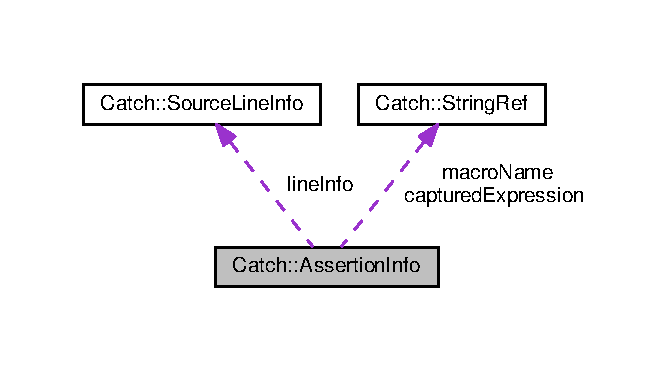
\includegraphics[width=321pt]{structCatch_1_1AssertionInfo__coll__graph}
\end{center}
\end{figure}
\subsection*{Public Attributes}
\begin{DoxyCompactItemize}
\item 
\hyperlink{classCatch_1_1StringRef}{String\+Ref} {\bfseries macro\+Name}\hypertarget{structCatch_1_1AssertionInfo_aaf3fbb9f1fe09c879ba3d877584e3056}{}\label{structCatch_1_1AssertionInfo_aaf3fbb9f1fe09c879ba3d877584e3056}

\item 
\hyperlink{structCatch_1_1SourceLineInfo}{Source\+Line\+Info} {\bfseries line\+Info}\hypertarget{structCatch_1_1AssertionInfo_a17bdbb404ba12658034f833be2f4c3e7}{}\label{structCatch_1_1AssertionInfo_a17bdbb404ba12658034f833be2f4c3e7}

\item 
\hyperlink{classCatch_1_1StringRef}{String\+Ref} {\bfseries captured\+Expression}\hypertarget{structCatch_1_1AssertionInfo_accd36744b4acaa3a691a72df0b42190f}{}\label{structCatch_1_1AssertionInfo_accd36744b4acaa3a691a72df0b42190f}

\item 
Result\+Disposition\+::\+Flags {\bfseries result\+Disposition}\hypertarget{structCatch_1_1AssertionInfo_a60353b3632ab2f827162f2b2d6911073}{}\label{structCatch_1_1AssertionInfo_a60353b3632ab2f827162f2b2d6911073}

\end{DoxyCompactItemize}


The documentation for this struct was generated from the following file\+:\begin{DoxyCompactItemize}
\item 
include/catch.\+hpp\end{DoxyCompactItemize}

\hypertarget{structCatch_1_1AssertionReaction}{}\section{Catch\+:\+:Assertion\+Reaction Struct Reference}
\label{structCatch_1_1AssertionReaction}\index{Catch\+::\+Assertion\+Reaction@{Catch\+::\+Assertion\+Reaction}}
\subsection*{Public Attributes}
\begin{DoxyCompactItemize}
\item 
bool {\bfseries should\+Debug\+Break} = false\hypertarget{structCatch_1_1AssertionReaction_adcf30fb90ff20d9789df78d424652497}{}\label{structCatch_1_1AssertionReaction_adcf30fb90ff20d9789df78d424652497}

\item 
bool {\bfseries should\+Throw} = false\hypertarget{structCatch_1_1AssertionReaction_a82c8d95a2c1b6a331bde66982a8e090f}{}\label{structCatch_1_1AssertionReaction_a82c8d95a2c1b6a331bde66982a8e090f}

\end{DoxyCompactItemize}


The documentation for this struct was generated from the following file\+:\begin{DoxyCompactItemize}
\item 
include/catch.\+hpp\end{DoxyCompactItemize}

\hypertarget{structCatch_1_1AutoReg}{}\section{Catch\+:\+:Auto\+Reg Struct Reference}
\label{structCatch_1_1AutoReg}\index{Catch\+::\+Auto\+Reg@{Catch\+::\+Auto\+Reg}}


Inheritance diagram for Catch\+:\+:Auto\+Reg\+:\nopagebreak
\begin{figure}[H]
\begin{center}
\leavevmode
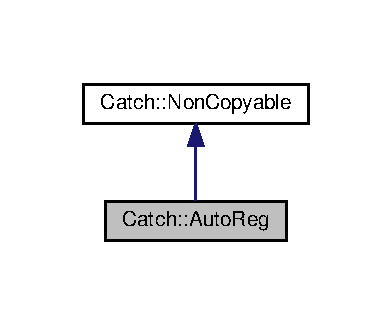
\includegraphics[width=188pt]{structCatch_1_1AutoReg__inherit__graph}
\end{center}
\end{figure}


Collaboration diagram for Catch\+:\+:Auto\+Reg\+:\nopagebreak
\begin{figure}[H]
\begin{center}
\leavevmode
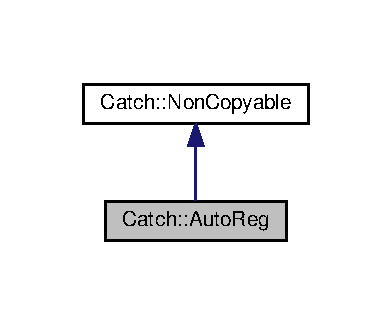
\includegraphics[width=188pt]{structCatch_1_1AutoReg__coll__graph}
\end{center}
\end{figure}
\subsection*{Public Member Functions}
\begin{DoxyCompactItemize}
\item 
{\bfseries Auto\+Reg} (\hyperlink{structCatch_1_1ITestInvoker}{I\+Test\+Invoker} $\ast$invoker, \hyperlink{structCatch_1_1SourceLineInfo}{Source\+Line\+Info} const \&line\+Info, \hyperlink{classCatch_1_1StringRef}{String\+Ref} const \&class\+Or\+Method, \hyperlink{structCatch_1_1NameAndTags}{Name\+And\+Tags} const \&name\+And\+Tags) noexcept\hypertarget{structCatch_1_1AutoReg_a7eba02fb9d80b9896bf5a6517369af28}{}\label{structCatch_1_1AutoReg_a7eba02fb9d80b9896bf5a6517369af28}

\end{DoxyCompactItemize}


The documentation for this struct was generated from the following file\+:\begin{DoxyCompactItemize}
\item 
include/catch.\+hpp\end{DoxyCompactItemize}

\hypertarget{classCatch_1_1BenchmarkLooper}{}\section{Catch\+:\+:Benchmark\+Looper Class Reference}
\label{classCatch_1_1BenchmarkLooper}\index{Catch\+::\+Benchmark\+Looper@{Catch\+::\+Benchmark\+Looper}}
\subsection*{Public Member Functions}
\begin{DoxyCompactItemize}
\item 
{\bfseries Benchmark\+Looper} (\hyperlink{classCatch_1_1StringRef}{String\+Ref} name)\hypertarget{classCatch_1_1BenchmarkLooper_ab9ba6397306a70082f39e63a8a71bde6}{}\label{classCatch_1_1BenchmarkLooper_ab9ba6397306a70082f39e63a8a71bde6}

\item 
{\bfseries operator bool} ()\hypertarget{classCatch_1_1BenchmarkLooper_a54da41bada9da038dc05faf41d746765}{}\label{classCatch_1_1BenchmarkLooper_a54da41bada9da038dc05faf41d746765}

\item 
void {\bfseries increment} ()\hypertarget{classCatch_1_1BenchmarkLooper_a210552aff5b19408637444d4bb35d59c}{}\label{classCatch_1_1BenchmarkLooper_a210552aff5b19408637444d4bb35d59c}

\item 
void {\bfseries report\+Start} ()\hypertarget{classCatch_1_1BenchmarkLooper_a0697d1b266112b110edf2025b82c4e77}{}\label{classCatch_1_1BenchmarkLooper_a0697d1b266112b110edf2025b82c4e77}

\item 
auto {\bfseries needs\+More\+Iterations} () -\/$>$ bool\hypertarget{classCatch_1_1BenchmarkLooper_a97bd944521f519b1593a5d1d2f9998fa}{}\label{classCatch_1_1BenchmarkLooper_a97bd944521f519b1593a5d1d2f9998fa}

\end{DoxyCompactItemize}


The documentation for this class was generated from the following file\+:\begin{DoxyCompactItemize}
\item 
include/catch.\+hpp\end{DoxyCompactItemize}

\hypertarget{classCatch_1_1BinaryExpr}{}\section{Catch\+:\+:Binary\+Expr$<$ LhsT, RhsT $>$ Class Template Reference}
\label{classCatch_1_1BinaryExpr}\index{Catch\+::\+Binary\+Expr$<$ Lhs\+T, Rhs\+T $>$@{Catch\+::\+Binary\+Expr$<$ Lhs\+T, Rhs\+T $>$}}


Inheritance diagram for Catch\+:\+:Binary\+Expr$<$ LhsT, RhsT $>$\+:
\nopagebreak
\begin{figure}[H]
\begin{center}
\leavevmode
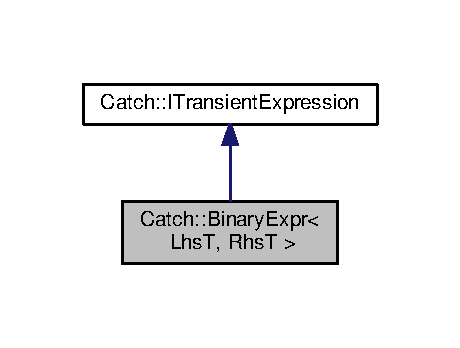
\includegraphics[width=221pt]{classCatch_1_1BinaryExpr__inherit__graph}
\end{center}
\end{figure}


Collaboration diagram for Catch\+:\+:Binary\+Expr$<$ LhsT, RhsT $>$\+:
\nopagebreak
\begin{figure}[H]
\begin{center}
\leavevmode
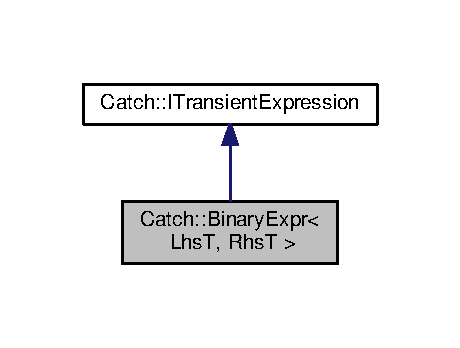
\includegraphics[width=221pt]{classCatch_1_1BinaryExpr__coll__graph}
\end{center}
\end{figure}
\subsection*{Public Member Functions}
\begin{DoxyCompactItemize}
\item 
{\bfseries Binary\+Expr} (bool comparison\+Result, LhsT lhs, \hyperlink{classCatch_1_1StringRef}{String\+Ref} op, RhsT rhs)\hypertarget{classCatch_1_1BinaryExpr_a657d66346aef97a760c22776fe6008b6}{}\label{classCatch_1_1BinaryExpr_a657d66346aef97a760c22776fe6008b6}

\end{DoxyCompactItemize}
\subsection*{Additional Inherited Members}


The documentation for this class was generated from the following file\+:\begin{DoxyCompactItemize}
\item 
include/catch.\+hpp\end{DoxyCompactItemize}

\hypertarget{classBTree}{}\section{B\+Tree Class Reference}
\label{classBTree}\index{B\+Tree@{B\+Tree}}
\subsection*{Public Member Functions}
\begin{DoxyCompactItemize}
\item 
\hyperlink{classBTree_ae3adf097939b1bce7fba5a5d55ff8907}{B\+Tree} ()
\begin{DoxyCompactList}\small\item\em A constructor that creates a binary tree with a root with an empty value. \end{DoxyCompactList}\item 
\hyperlink{classBTree_a3278f51f6a7719e17b2e2b17be41f324}{B\+Tree} (string initial\+\_\+text)
\begin{DoxyCompactList}\small\item\em A constructor that creates a binary tree with a root with an given value. \end{DoxyCompactList}\item 
P\+String\+Node {\bfseries get\+Root} (void)\hypertarget{classBTree_ada02034e08407da08fc3715ca84aeed4}{}\label{classBTree_ada02034e08407da08fc3715ca84aeed4}

\end{DoxyCompactItemize}


\subsection{Constructor \& Destructor Documentation}
\index{B\+Tree@{B\+Tree}!B\+Tree@{B\+Tree}}
\index{B\+Tree@{B\+Tree}!B\+Tree@{B\+Tree}}
\subsubsection[{\texorpdfstring{B\+Tree()}{BTree()}}]{\setlength{\rightskip}{0pt plus 5cm}B\+Tree\+::\+B\+Tree (
\begin{DoxyParamCaption}
\item[{void}]{}
\end{DoxyParamCaption}
)}\hypertarget{classBTree_ae3adf097939b1bce7fba5a5d55ff8907}{}\label{classBTree_ae3adf097939b1bce7fba5a5d55ff8907}


A constructor that creates a binary tree with a root with an empty value. 

Creates a new binary tree and creates a new node to be it\textquotesingle{}s root. The root value is empty. \index{B\+Tree@{B\+Tree}!B\+Tree@{B\+Tree}}
\index{B\+Tree@{B\+Tree}!B\+Tree@{B\+Tree}}
\subsubsection[{\texorpdfstring{B\+Tree(string initial\+\_\+text)}{BTree(string initial_text)}}]{\setlength{\rightskip}{0pt plus 5cm}B\+Tree\+::\+B\+Tree (
\begin{DoxyParamCaption}
\item[{string}]{initial\+Text}
\end{DoxyParamCaption}
)}\hypertarget{classBTree_a3278f51f6a7719e17b2e2b17be41f324}{}\label{classBTree_a3278f51f6a7719e17b2e2b17be41f324}


A constructor that creates a binary tree with a root with an given value. 

Creates a new binary tree and creates a new node to be it\textquotesingle{}s root. The root value is given as param. 
\begin{DoxyParams}{Parameters}
{\em (\+The} & only explicit interface) A valid and already allocated string. \\
\hline
\end{DoxyParams}


The documentation for this class was generated from the following files\+:\begin{DoxyCompactItemize}
\item 
include/btree.\+hpp\item 
src/\hyperlink{btree_8cpp}{btree.\+cpp}\end{DoxyCompactItemize}

\hypertarget{structCatch_1_1Matchers_1_1StdString_1_1CasedString}{}\section{Catch\+:\+:Matchers\+:\+:Std\+String\+:\+:Cased\+String Struct Reference}
\label{structCatch_1_1Matchers_1_1StdString_1_1CasedString}\index{Catch\+::\+Matchers\+::\+Std\+String\+::\+Cased\+String@{Catch\+::\+Matchers\+::\+Std\+String\+::\+Cased\+String}}


Collaboration diagram for Catch\+:\+:Matchers\+:\+:Std\+String\+:\+:Cased\+String\+:\nopagebreak
\begin{figure}[H]
\begin{center}
\leavevmode
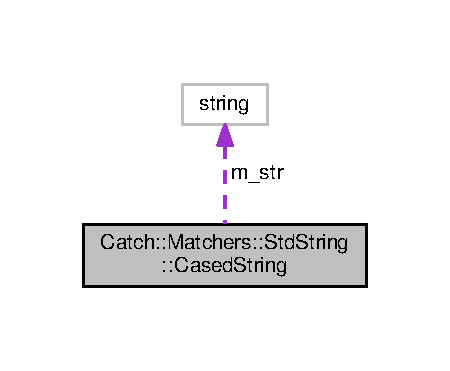
\includegraphics[width=216pt]{structCatch_1_1Matchers_1_1StdString_1_1CasedString__coll__graph}
\end{center}
\end{figure}
\subsection*{Public Member Functions}
\begin{DoxyCompactItemize}
\item 
{\bfseries Cased\+String} (std\+::string const \&str, Case\+Sensitive\+::\+Choice case\+Sensitivity)\hypertarget{structCatch_1_1Matchers_1_1StdString_1_1CasedString_aa88bbc5acd2bff22351d8d4b1816b561}{}\label{structCatch_1_1Matchers_1_1StdString_1_1CasedString_aa88bbc5acd2bff22351d8d4b1816b561}

\item 
std\+::string {\bfseries adjust\+String} (std\+::string const \&str) const \hypertarget{structCatch_1_1Matchers_1_1StdString_1_1CasedString_a0ff84e194426c8f4bca0660b9180d20d}{}\label{structCatch_1_1Matchers_1_1StdString_1_1CasedString_a0ff84e194426c8f4bca0660b9180d20d}

\item 
std\+::string {\bfseries case\+Sensitivity\+Suffix} () const \hypertarget{structCatch_1_1Matchers_1_1StdString_1_1CasedString_a1113c80dd02967032a99290bdcd1b590}{}\label{structCatch_1_1Matchers_1_1StdString_1_1CasedString_a1113c80dd02967032a99290bdcd1b590}

\end{DoxyCompactItemize}
\subsection*{Public Attributes}
\begin{DoxyCompactItemize}
\item 
Case\+Sensitive\+::\+Choice {\bfseries m\+\_\+case\+Sensitivity}\hypertarget{structCatch_1_1Matchers_1_1StdString_1_1CasedString_ae1c2864c986941536a6e94cca0528f92}{}\label{structCatch_1_1Matchers_1_1StdString_1_1CasedString_ae1c2864c986941536a6e94cca0528f92}

\item 
std\+::string {\bfseries m\+\_\+str}\hypertarget{structCatch_1_1Matchers_1_1StdString_1_1CasedString_ad05dbc99aba3c3c386d6b856b213f911}{}\label{structCatch_1_1Matchers_1_1StdString_1_1CasedString_ad05dbc99aba3c3c386d6b856b213f911}

\end{DoxyCompactItemize}


The documentation for this struct was generated from the following file\+:\begin{DoxyCompactItemize}
\item 
include/catch.\+hpp\end{DoxyCompactItemize}

\hypertarget{structCatch_1_1CaseSensitive}{}\section{Catch\+:\+:Case\+Sensitive Struct Reference}
\label{structCatch_1_1CaseSensitive}\index{Catch\+::\+Case\+Sensitive@{Catch\+::\+Case\+Sensitive}}
\subsection*{Public Types}
\begin{DoxyCompactItemize}
\item 
enum {\bfseries Choice} \{ {\bfseries Yes}, 
{\bfseries No}
 \}\hypertarget{structCatch_1_1CaseSensitive_aad49d3aee2d97066642fffa919685c6a}{}\label{structCatch_1_1CaseSensitive_aad49d3aee2d97066642fffa919685c6a}

\end{DoxyCompactItemize}


The documentation for this struct was generated from the following file\+:\begin{DoxyCompactItemize}
\item 
include/catch.\+hpp\end{DoxyCompactItemize}

\hypertarget{structCatch__global__namespace__dummy}{}\section{Catch\+\_\+global\+\_\+namespace\+\_\+dummy Struct Reference}
\label{structCatch__global__namespace__dummy}\index{Catch\+\_\+global\+\_\+namespace\+\_\+dummy@{Catch\+\_\+global\+\_\+namespace\+\_\+dummy}}


The documentation for this struct was generated from the following file\+:\begin{DoxyCompactItemize}
\item 
include/catch.\+hpp\end{DoxyCompactItemize}

\hypertarget{structCatch_1_1Matchers_1_1Vector_1_1ContainsElementMatcher}{}\section{Catch\+:\+:Matchers\+:\+:Vector\+:\+:Contains\+Element\+Matcher$<$ T $>$ Struct Template Reference}
\label{structCatch_1_1Matchers_1_1Vector_1_1ContainsElementMatcher}\index{Catch\+::\+Matchers\+::\+Vector\+::\+Contains\+Element\+Matcher$<$ T $>$@{Catch\+::\+Matchers\+::\+Vector\+::\+Contains\+Element\+Matcher$<$ T $>$}}


Inheritance diagram for Catch\+:\+:Matchers\+:\+:Vector\+:\+:Contains\+Element\+Matcher$<$ T $>$\+:\nopagebreak
\begin{figure}[H]
\begin{center}
\leavevmode
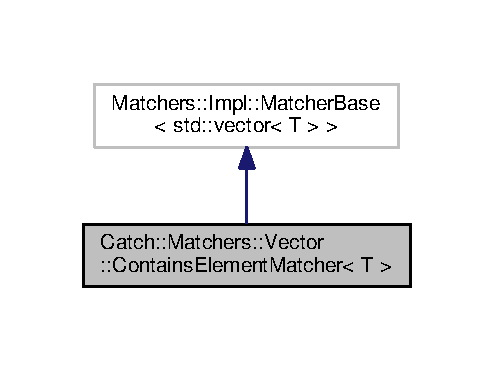
\includegraphics[width=237pt]{structCatch_1_1Matchers_1_1Vector_1_1ContainsElementMatcher__inherit__graph}
\end{center}
\end{figure}


Collaboration diagram for Catch\+:\+:Matchers\+:\+:Vector\+:\+:Contains\+Element\+Matcher$<$ T $>$\+:\nopagebreak
\begin{figure}[H]
\begin{center}
\leavevmode
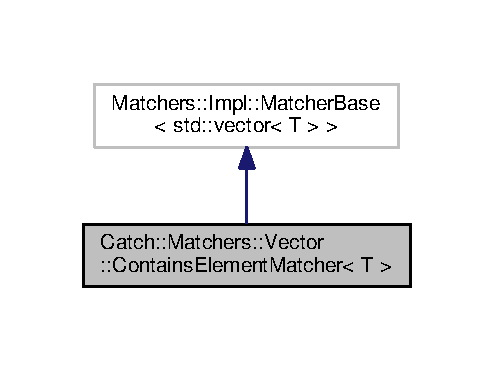
\includegraphics[width=237pt]{structCatch_1_1Matchers_1_1Vector_1_1ContainsElementMatcher__coll__graph}
\end{center}
\end{figure}
\subsection*{Public Member Functions}
\begin{DoxyCompactItemize}
\item 
{\bfseries Contains\+Element\+Matcher} (T const \&comparator)\hypertarget{structCatch_1_1Matchers_1_1Vector_1_1ContainsElementMatcher_a6a05740b5d3f89fac8de84ac0cff7b93}{}\label{structCatch_1_1Matchers_1_1Vector_1_1ContainsElementMatcher_a6a05740b5d3f89fac8de84ac0cff7b93}

\item 
bool {\bfseries match} (std\+::vector$<$ T $>$ const \&v) const override\hypertarget{structCatch_1_1Matchers_1_1Vector_1_1ContainsElementMatcher_a6a4be6e5642e267433d370649beb0fac}{}\label{structCatch_1_1Matchers_1_1Vector_1_1ContainsElementMatcher_a6a4be6e5642e267433d370649beb0fac}

\item 
std\+::string {\bfseries describe} () const override\hypertarget{structCatch_1_1Matchers_1_1Vector_1_1ContainsElementMatcher_aea3b674389a0afd82af6ba4b10f86ae6}{}\label{structCatch_1_1Matchers_1_1Vector_1_1ContainsElementMatcher_aea3b674389a0afd82af6ba4b10f86ae6}

\end{DoxyCompactItemize}
\subsection*{Public Attributes}
\begin{DoxyCompactItemize}
\item 
T const \& {\bfseries m\+\_\+comparator}\hypertarget{structCatch_1_1Matchers_1_1Vector_1_1ContainsElementMatcher_ab7eada6c4bbce1d21b44773262f9cb23}{}\label{structCatch_1_1Matchers_1_1Vector_1_1ContainsElementMatcher_ab7eada6c4bbce1d21b44773262f9cb23}

\end{DoxyCompactItemize}


The documentation for this struct was generated from the following file\+:\begin{DoxyCompactItemize}
\item 
include/catch.\+hpp\end{DoxyCompactItemize}

\hypertarget{structCatch_1_1Matchers_1_1StdString_1_1ContainsMatcher}{}\section{Catch\+:\+:Matchers\+:\+:Std\+String\+:\+:Contains\+Matcher Struct Reference}
\label{structCatch_1_1Matchers_1_1StdString_1_1ContainsMatcher}\index{Catch\+::\+Matchers\+::\+Std\+String\+::\+Contains\+Matcher@{Catch\+::\+Matchers\+::\+Std\+String\+::\+Contains\+Matcher}}


Inheritance diagram for Catch\+:\+:Matchers\+:\+:Std\+String\+:\+:Contains\+Matcher\+:\nopagebreak
\begin{figure}[H]
\begin{center}
\leavevmode
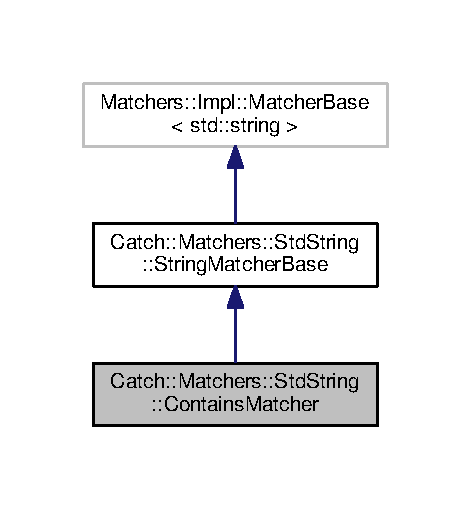
\includegraphics[width=226pt]{structCatch_1_1Matchers_1_1StdString_1_1ContainsMatcher__inherit__graph}
\end{center}
\end{figure}


Collaboration diagram for Catch\+:\+:Matchers\+:\+:Std\+String\+:\+:Contains\+Matcher\+:\nopagebreak
\begin{figure}[H]
\begin{center}
\leavevmode
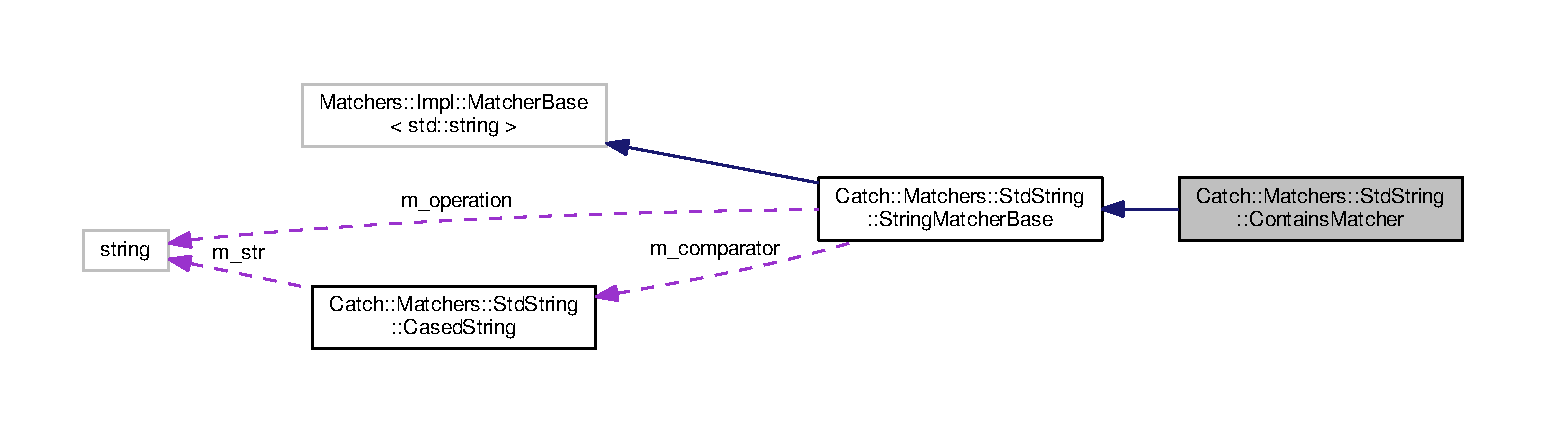
\includegraphics[width=350pt]{structCatch_1_1Matchers_1_1StdString_1_1ContainsMatcher__coll__graph}
\end{center}
\end{figure}
\subsection*{Public Member Functions}
\begin{DoxyCompactItemize}
\item 
{\bfseries Contains\+Matcher} (\hyperlink{structCatch_1_1Matchers_1_1StdString_1_1CasedString}{Cased\+String} const \&comparator)\hypertarget{structCatch_1_1Matchers_1_1StdString_1_1ContainsMatcher_acc892883c8409e34b28c9b39d4ef1fe3}{}\label{structCatch_1_1Matchers_1_1StdString_1_1ContainsMatcher_acc892883c8409e34b28c9b39d4ef1fe3}

\item 
bool {\bfseries match} (std\+::string const \&source) const override\hypertarget{structCatch_1_1Matchers_1_1StdString_1_1ContainsMatcher_a630628b234b037be83fe587081a80b53}{}\label{structCatch_1_1Matchers_1_1StdString_1_1ContainsMatcher_a630628b234b037be83fe587081a80b53}

\end{DoxyCompactItemize}
\subsection*{Additional Inherited Members}


The documentation for this struct was generated from the following file\+:\begin{DoxyCompactItemize}
\item 
include/catch.\+hpp\end{DoxyCompactItemize}

\hypertarget{structCatch_1_1Matchers_1_1Vector_1_1ContainsMatcher}{}\section{Catch\+:\+:Matchers\+:\+:Vector\+:\+:Contains\+Matcher$<$ T $>$ Struct Template Reference}
\label{structCatch_1_1Matchers_1_1Vector_1_1ContainsMatcher}\index{Catch\+::\+Matchers\+::\+Vector\+::\+Contains\+Matcher$<$ T $>$@{Catch\+::\+Matchers\+::\+Vector\+::\+Contains\+Matcher$<$ T $>$}}


Inheritance diagram for Catch\+:\+:Matchers\+:\+:Vector\+:\+:Contains\+Matcher$<$ T $>$\+:
\nopagebreak
\begin{figure}[H]
\begin{center}
\leavevmode
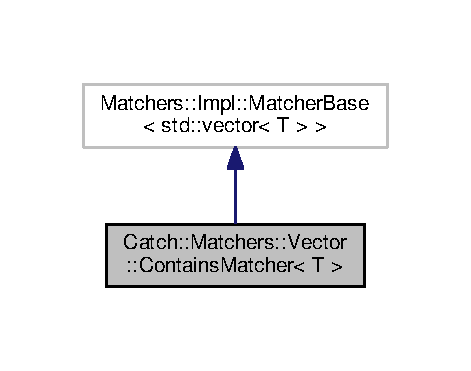
\includegraphics[width=226pt]{structCatch_1_1Matchers_1_1Vector_1_1ContainsMatcher__inherit__graph}
\end{center}
\end{figure}


Collaboration diagram for Catch\+:\+:Matchers\+:\+:Vector\+:\+:Contains\+Matcher$<$ T $>$\+:
\nopagebreak
\begin{figure}[H]
\begin{center}
\leavevmode
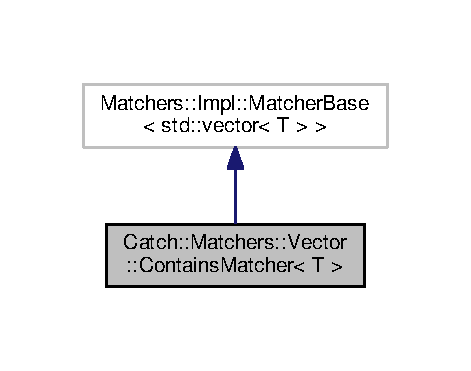
\includegraphics[width=226pt]{structCatch_1_1Matchers_1_1Vector_1_1ContainsMatcher__coll__graph}
\end{center}
\end{figure}
\subsection*{Public Member Functions}
\begin{DoxyCompactItemize}
\item 
{\bfseries Contains\+Matcher} (std\+::vector$<$ T $>$ const \&comparator)\hypertarget{structCatch_1_1Matchers_1_1Vector_1_1ContainsMatcher_ad8e92c8399be6dce75bb5702cdfab700}{}\label{structCatch_1_1Matchers_1_1Vector_1_1ContainsMatcher_ad8e92c8399be6dce75bb5702cdfab700}

\item 
bool {\bfseries match} (std\+::vector$<$ T $>$ const \&v) const override\hypertarget{structCatch_1_1Matchers_1_1Vector_1_1ContainsMatcher_afd33467ae48a41a634572b41b053f67f}{}\label{structCatch_1_1Matchers_1_1Vector_1_1ContainsMatcher_afd33467ae48a41a634572b41b053f67f}

\item 
std\+::string {\bfseries describe} () const override\hypertarget{structCatch_1_1Matchers_1_1Vector_1_1ContainsMatcher_abe6a9ea3d6506c9a1f75ff524f35832e}{}\label{structCatch_1_1Matchers_1_1Vector_1_1ContainsMatcher_abe6a9ea3d6506c9a1f75ff524f35832e}

\end{DoxyCompactItemize}
\subsection*{Public Attributes}
\begin{DoxyCompactItemize}
\item 
std\+::vector$<$ T $>$ const \& {\bfseries m\+\_\+comparator}\hypertarget{structCatch_1_1Matchers_1_1Vector_1_1ContainsMatcher_a83d051166e4ed0d535219ad6ee99abb2}{}\label{structCatch_1_1Matchers_1_1Vector_1_1ContainsMatcher_a83d051166e4ed0d535219ad6ee99abb2}

\end{DoxyCompactItemize}


The documentation for this struct was generated from the following file\+:\begin{DoxyCompactItemize}
\item 
include/catch.\+hpp\end{DoxyCompactItemize}

\hypertarget{structCatch_1_1Counts}{}\section{Catch\+:\+:Counts Struct Reference}
\label{structCatch_1_1Counts}\index{Catch\+::\+Counts@{Catch\+::\+Counts}}
\subsection*{Public Member Functions}
\begin{DoxyCompactItemize}
\item 
\hyperlink{structCatch_1_1Counts}{Counts} {\bfseries operator-\/} (\hyperlink{structCatch_1_1Counts}{Counts} const \&other) const \hypertarget{structCatch_1_1Counts_aedf86fefe33938d132a6981171cd83e6}{}\label{structCatch_1_1Counts_aedf86fefe33938d132a6981171cd83e6}

\item 
\hyperlink{structCatch_1_1Counts}{Counts} \& {\bfseries operator+=} (\hyperlink{structCatch_1_1Counts}{Counts} const \&other)\hypertarget{structCatch_1_1Counts_a322a89475cd2cc039140ef371e973677}{}\label{structCatch_1_1Counts_a322a89475cd2cc039140ef371e973677}

\item 
std\+::size\+\_\+t {\bfseries total} () const \hypertarget{structCatch_1_1Counts_a9125c662e30114e5c5cc94729b1e9e84}{}\label{structCatch_1_1Counts_a9125c662e30114e5c5cc94729b1e9e84}

\item 
bool {\bfseries all\+Passed} () const \hypertarget{structCatch_1_1Counts_adbbaca552f6017ce69e0d5dc5500bea4}{}\label{structCatch_1_1Counts_adbbaca552f6017ce69e0d5dc5500bea4}

\item 
bool {\bfseries all\+Ok} () const \hypertarget{structCatch_1_1Counts_ab2497c9dfc77be757a90225ea69595f5}{}\label{structCatch_1_1Counts_ab2497c9dfc77be757a90225ea69595f5}

\end{DoxyCompactItemize}
\subsection*{Public Attributes}
\begin{DoxyCompactItemize}
\item 
std\+::size\+\_\+t {\bfseries passed} = 0\hypertarget{structCatch_1_1Counts_ad28daaf3de28006400208b6dd0c631e6}{}\label{structCatch_1_1Counts_ad28daaf3de28006400208b6dd0c631e6}

\item 
std\+::size\+\_\+t {\bfseries failed} = 0\hypertarget{structCatch_1_1Counts_a19982a3817a3bc2c07f0290e71f497a3}{}\label{structCatch_1_1Counts_a19982a3817a3bc2c07f0290e71f497a3}

\item 
std\+::size\+\_\+t {\bfseries failed\+But\+Ok} = 0\hypertarget{structCatch_1_1Counts_ac090973a2ff51394cd452718e75c073e}{}\label{structCatch_1_1Counts_ac090973a2ff51394cd452718e75c073e}

\end{DoxyCompactItemize}


The documentation for this struct was generated from the following file\+:\begin{DoxyCompactItemize}
\item 
include/catch.\+hpp\end{DoxyCompactItemize}

\hypertarget{structCatch_1_1Decomposer}{}\section{Catch\+:\+:Decomposer Struct Reference}
\label{structCatch_1_1Decomposer}\index{Catch\+::\+Decomposer@{Catch\+::\+Decomposer}}
\subsection*{Public Member Functions}
\begin{DoxyCompactItemize}
\item 
{\footnotesize template$<$typename T $>$ }\\auto {\bfseries operator$<$=} (T const \&lhs) -\/$>$ \hyperlink{classCatch_1_1ExprLhs}{Expr\+Lhs}$<$ T const \& $>$\hypertarget{structCatch_1_1Decomposer_a4b1e5e844c20e5a90e3d759d216674cd}{}\label{structCatch_1_1Decomposer_a4b1e5e844c20e5a90e3d759d216674cd}

\item 
auto {\bfseries operator$<$=} (bool value) -\/$>$ \hyperlink{classCatch_1_1ExprLhs}{Expr\+Lhs}$<$ bool $>$\hypertarget{structCatch_1_1Decomposer_aac129b94903ae1339d5709049d83613b}{}\label{structCatch_1_1Decomposer_aac129b94903ae1339d5709049d83613b}

\end{DoxyCompactItemize}


The documentation for this struct was generated from the following file\+:\begin{DoxyCompactItemize}
\item 
include/catch.\+hpp\end{DoxyCompactItemize}

\hypertarget{structCatch_1_1Matchers_1_1StdString_1_1EndsWithMatcher}{}\section{Catch\+:\+:Matchers\+:\+:Std\+String\+:\+:Ends\+With\+Matcher Struct Reference}
\label{structCatch_1_1Matchers_1_1StdString_1_1EndsWithMatcher}\index{Catch\+::\+Matchers\+::\+Std\+String\+::\+Ends\+With\+Matcher@{Catch\+::\+Matchers\+::\+Std\+String\+::\+Ends\+With\+Matcher}}


Inheritance diagram for Catch\+:\+:Matchers\+:\+:Std\+String\+:\+:Ends\+With\+Matcher\+:
\nopagebreak
\begin{figure}[H]
\begin{center}
\leavevmode
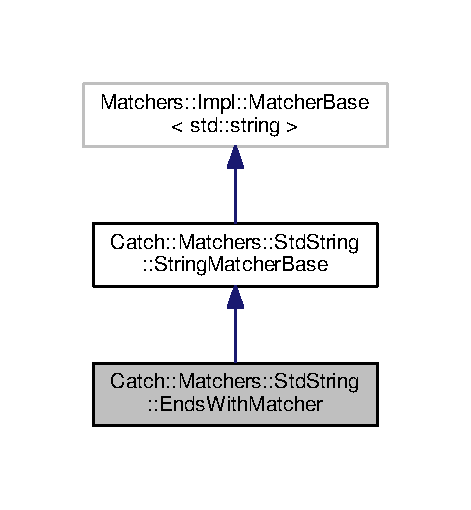
\includegraphics[width=226pt]{structCatch_1_1Matchers_1_1StdString_1_1EndsWithMatcher__inherit__graph}
\end{center}
\end{figure}


Collaboration diagram for Catch\+:\+:Matchers\+:\+:Std\+String\+:\+:Ends\+With\+Matcher\+:
\nopagebreak
\begin{figure}[H]
\begin{center}
\leavevmode
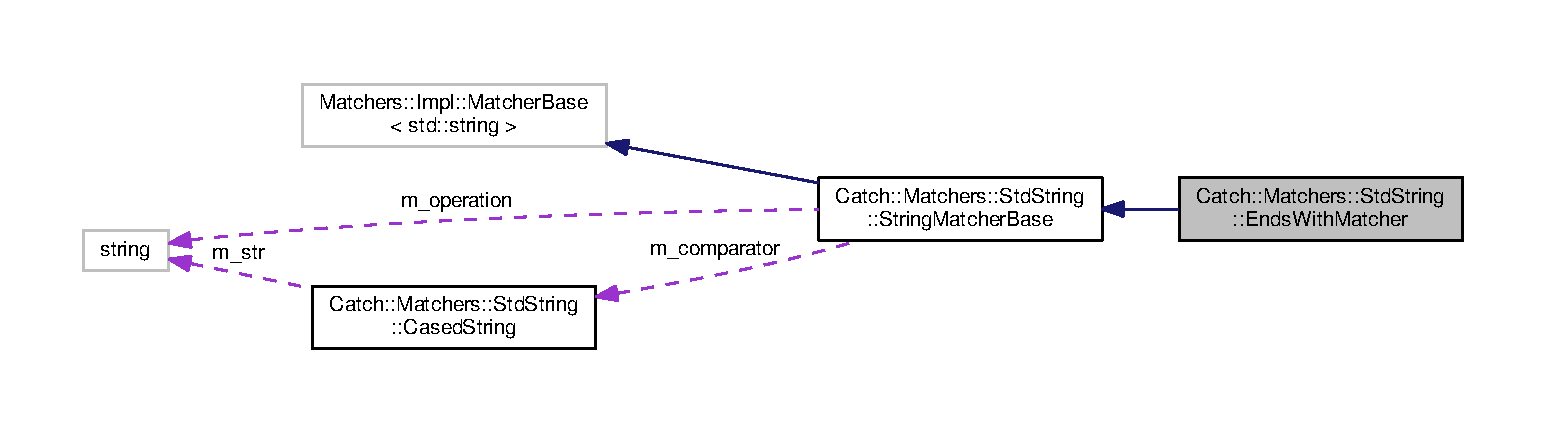
\includegraphics[width=350pt]{structCatch_1_1Matchers_1_1StdString_1_1EndsWithMatcher__coll__graph}
\end{center}
\end{figure}
\subsection*{Public Member Functions}
\begin{DoxyCompactItemize}
\item 
{\bfseries Ends\+With\+Matcher} (\hyperlink{structCatch_1_1Matchers_1_1StdString_1_1CasedString}{Cased\+String} const \&comparator)\hypertarget{structCatch_1_1Matchers_1_1StdString_1_1EndsWithMatcher_aa5ec700b4629562f74f362080accfd7b}{}\label{structCatch_1_1Matchers_1_1StdString_1_1EndsWithMatcher_aa5ec700b4629562f74f362080accfd7b}

\item 
bool {\bfseries match} (std\+::string const \&source) const override\hypertarget{structCatch_1_1Matchers_1_1StdString_1_1EndsWithMatcher_aca2741fa57374a2a98d2a84ac3e13a6d}{}\label{structCatch_1_1Matchers_1_1StdString_1_1EndsWithMatcher_aca2741fa57374a2a98d2a84ac3e13a6d}

\end{DoxyCompactItemize}
\subsection*{Additional Inherited Members}


The documentation for this struct was generated from the following file\+:\begin{DoxyCompactItemize}
\item 
include/catch.\+hpp\end{DoxyCompactItemize}

\hypertarget{structCatch_1_1Matchers_1_1StdString_1_1EqualsMatcher}{}\section{Catch\+:\+:Matchers\+:\+:Std\+String\+:\+:Equals\+Matcher Struct Reference}
\label{structCatch_1_1Matchers_1_1StdString_1_1EqualsMatcher}\index{Catch\+::\+Matchers\+::\+Std\+String\+::\+Equals\+Matcher@{Catch\+::\+Matchers\+::\+Std\+String\+::\+Equals\+Matcher}}


Inheritance diagram for Catch\+:\+:Matchers\+:\+:Std\+String\+:\+:Equals\+Matcher\+:\nopagebreak
\begin{figure}[H]
\begin{center}
\leavevmode
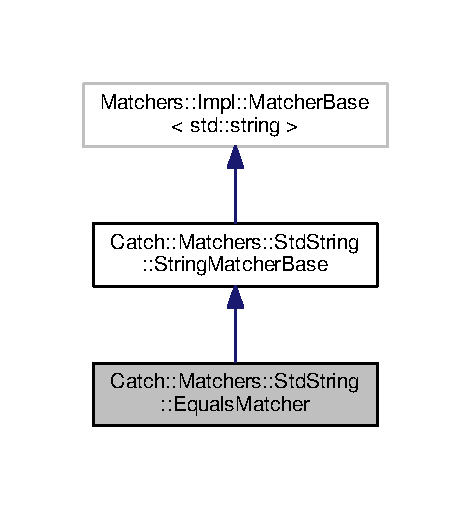
\includegraphics[width=226pt]{structCatch_1_1Matchers_1_1StdString_1_1EqualsMatcher__inherit__graph}
\end{center}
\end{figure}


Collaboration diagram for Catch\+:\+:Matchers\+:\+:Std\+String\+:\+:Equals\+Matcher\+:\nopagebreak
\begin{figure}[H]
\begin{center}
\leavevmode
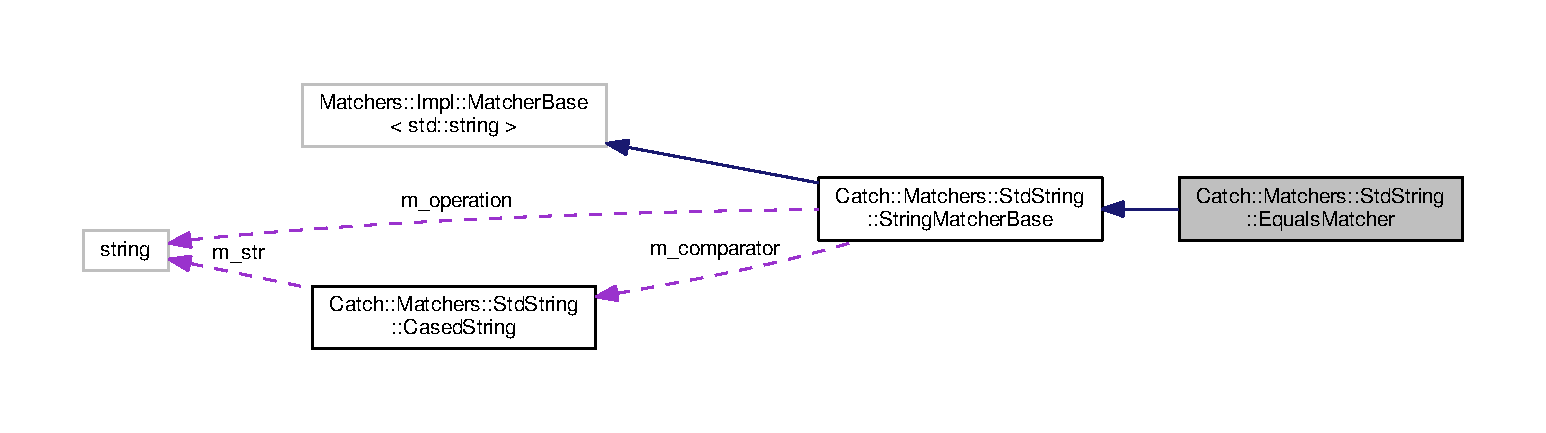
\includegraphics[width=350pt]{structCatch_1_1Matchers_1_1StdString_1_1EqualsMatcher__coll__graph}
\end{center}
\end{figure}
\subsection*{Public Member Functions}
\begin{DoxyCompactItemize}
\item 
{\bfseries Equals\+Matcher} (\hyperlink{structCatch_1_1Matchers_1_1StdString_1_1CasedString}{Cased\+String} const \&comparator)\hypertarget{structCatch_1_1Matchers_1_1StdString_1_1EqualsMatcher_ab740f1fb2310e9fe3fed5134d4c7e4c8}{}\label{structCatch_1_1Matchers_1_1StdString_1_1EqualsMatcher_ab740f1fb2310e9fe3fed5134d4c7e4c8}

\item 
bool {\bfseries match} (std\+::string const \&source) const override\hypertarget{structCatch_1_1Matchers_1_1StdString_1_1EqualsMatcher_a0bb9d64693f7bb1ef7441062d219f21a}{}\label{structCatch_1_1Matchers_1_1StdString_1_1EqualsMatcher_a0bb9d64693f7bb1ef7441062d219f21a}

\end{DoxyCompactItemize}
\subsection*{Additional Inherited Members}


The documentation for this struct was generated from the following file\+:\begin{DoxyCompactItemize}
\item 
include/catch.\+hpp\end{DoxyCompactItemize}

\hypertarget{structCatch_1_1Matchers_1_1Vector_1_1EqualsMatcher}{}\section{Catch\+:\+:Matchers\+:\+:Vector\+:\+:Equals\+Matcher$<$ T $>$ Struct Template Reference}
\label{structCatch_1_1Matchers_1_1Vector_1_1EqualsMatcher}\index{Catch\+::\+Matchers\+::\+Vector\+::\+Equals\+Matcher$<$ T $>$@{Catch\+::\+Matchers\+::\+Vector\+::\+Equals\+Matcher$<$ T $>$}}


Inheritance diagram for Catch\+:\+:Matchers\+:\+:Vector\+:\+:Equals\+Matcher$<$ T $>$\+:\nopagebreak
\begin{figure}[H]
\begin{center}
\leavevmode
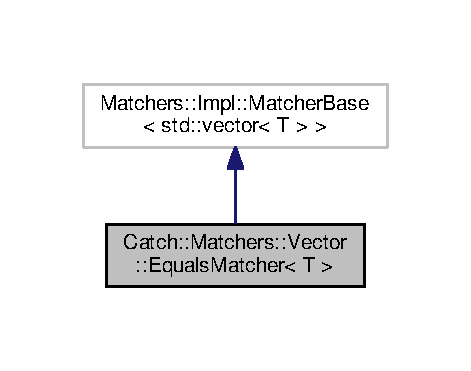
\includegraphics[width=226pt]{structCatch_1_1Matchers_1_1Vector_1_1EqualsMatcher__inherit__graph}
\end{center}
\end{figure}


Collaboration diagram for Catch\+:\+:Matchers\+:\+:Vector\+:\+:Equals\+Matcher$<$ T $>$\+:\nopagebreak
\begin{figure}[H]
\begin{center}
\leavevmode
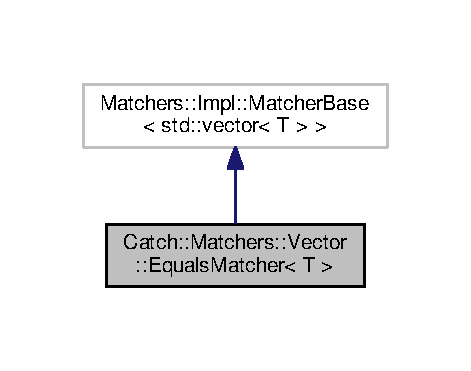
\includegraphics[width=226pt]{structCatch_1_1Matchers_1_1Vector_1_1EqualsMatcher__coll__graph}
\end{center}
\end{figure}
\subsection*{Public Member Functions}
\begin{DoxyCompactItemize}
\item 
{\bfseries Equals\+Matcher} (std\+::vector$<$ T $>$ const \&comparator)\hypertarget{structCatch_1_1Matchers_1_1Vector_1_1EqualsMatcher_a3846c47780d1991dcfe87aefded98008}{}\label{structCatch_1_1Matchers_1_1Vector_1_1EqualsMatcher_a3846c47780d1991dcfe87aefded98008}

\item 
bool {\bfseries match} (std\+::vector$<$ T $>$ const \&v) const override\hypertarget{structCatch_1_1Matchers_1_1Vector_1_1EqualsMatcher_a2d96cca58a44151fddc5257eda3305da}{}\label{structCatch_1_1Matchers_1_1Vector_1_1EqualsMatcher_a2d96cca58a44151fddc5257eda3305da}

\item 
std\+::string {\bfseries describe} () const override\hypertarget{structCatch_1_1Matchers_1_1Vector_1_1EqualsMatcher_a36b5f7ecada4081d6c65bebe8ddea6f4}{}\label{structCatch_1_1Matchers_1_1Vector_1_1EqualsMatcher_a36b5f7ecada4081d6c65bebe8ddea6f4}

\end{DoxyCompactItemize}
\subsection*{Public Attributes}
\begin{DoxyCompactItemize}
\item 
std\+::vector$<$ T $>$ const \& {\bfseries m\+\_\+comparator}\hypertarget{structCatch_1_1Matchers_1_1Vector_1_1EqualsMatcher_a56f7aa6f110a12b1b9aeb0cabbc9d755}{}\label{structCatch_1_1Matchers_1_1Vector_1_1EqualsMatcher_a56f7aa6f110a12b1b9aeb0cabbc9d755}

\end{DoxyCompactItemize}


The documentation for this struct was generated from the following file\+:\begin{DoxyCompactItemize}
\item 
include/catch.\+hpp\end{DoxyCompactItemize}

\hypertarget{classCatch_1_1ExceptionTranslatorRegistrar}{}\section{Catch\+:\+:Exception\+Translator\+Registrar Class Reference}
\label{classCatch_1_1ExceptionTranslatorRegistrar}\index{Catch\+::\+Exception\+Translator\+Registrar@{Catch\+::\+Exception\+Translator\+Registrar}}
\subsection*{Public Member Functions}
\begin{DoxyCompactItemize}
\item 
{\footnotesize template$<$typename T $>$ }\\{\bfseries Exception\+Translator\+Registrar} (std\+::string($\ast$translate\+Function)(T \&))\hypertarget{classCatch_1_1ExceptionTranslatorRegistrar_aa73229de911f26b1df6c6c87c4d9e04e}{}\label{classCatch_1_1ExceptionTranslatorRegistrar_aa73229de911f26b1df6c6c87c4d9e04e}

\end{DoxyCompactItemize}


The documentation for this class was generated from the following file\+:\begin{DoxyCompactItemize}
\item 
include/catch.\+hpp\end{DoxyCompactItemize}

\hypertarget{classCatch_1_1ExprLhs}{}\section{Catch\+:\+:Expr\+Lhs$<$ LhsT $>$ Class Template Reference}
\label{classCatch_1_1ExprLhs}\index{Catch\+::\+Expr\+Lhs$<$ Lhs\+T $>$@{Catch\+::\+Expr\+Lhs$<$ Lhs\+T $>$}}
\subsection*{Public Member Functions}
\begin{DoxyCompactItemize}
\item 
{\bfseries Expr\+Lhs} (LhsT lhs)\hypertarget{classCatch_1_1ExprLhs_ad22c6af1a7d6993240624d299714a479}{}\label{classCatch_1_1ExprLhs_ad22c6af1a7d6993240624d299714a479}

\item 
{\footnotesize template$<$typename RhsT $>$ }\\auto {\bfseries operator==} (RhsT const \&rhs) -\/$>$ \hyperlink{classCatch_1_1BinaryExpr}{Binary\+Expr}$<$ LhsT, RhsT const \& $>$ const \hypertarget{classCatch_1_1ExprLhs_a96537b7d47cf4567fff40d96637f9b96}{}\label{classCatch_1_1ExprLhs_a96537b7d47cf4567fff40d96637f9b96}

\item 
auto {\bfseries operator==} (bool rhs) -\/$>$ \hyperlink{classCatch_1_1BinaryExpr}{Binary\+Expr}$<$ LhsT, bool $>$ const \hypertarget{classCatch_1_1ExprLhs_ac400741dd25a7b2f00996c7bc48b2075}{}\label{classCatch_1_1ExprLhs_ac400741dd25a7b2f00996c7bc48b2075}

\item 
{\footnotesize template$<$typename RhsT $>$ }\\auto {\bfseries operator!=} (RhsT const \&rhs) -\/$>$ \hyperlink{classCatch_1_1BinaryExpr}{Binary\+Expr}$<$ LhsT, RhsT const \& $>$ const \hypertarget{classCatch_1_1ExprLhs_a3ad517cc72c85ae7d06e7a081a3c6cb8}{}\label{classCatch_1_1ExprLhs_a3ad517cc72c85ae7d06e7a081a3c6cb8}

\item 
auto {\bfseries operator!=} (bool rhs) -\/$>$ \hyperlink{classCatch_1_1BinaryExpr}{Binary\+Expr}$<$ LhsT, bool $>$ const \hypertarget{classCatch_1_1ExprLhs_af45381c45e92bc8182e8790d8b1396b9}{}\label{classCatch_1_1ExprLhs_af45381c45e92bc8182e8790d8b1396b9}

\item 
{\footnotesize template$<$typename RhsT $>$ }\\auto {\bfseries operator$>$} (RhsT const \&rhs) -\/$>$ \hyperlink{classCatch_1_1BinaryExpr}{Binary\+Expr}$<$ LhsT, RhsT const \& $>$ const \hypertarget{classCatch_1_1ExprLhs_aff0149e0c0376f9b2e6763f7fefc5c60}{}\label{classCatch_1_1ExprLhs_aff0149e0c0376f9b2e6763f7fefc5c60}

\item 
{\footnotesize template$<$typename RhsT $>$ }\\auto {\bfseries operator$<$} (RhsT const \&rhs) -\/$>$ \hyperlink{classCatch_1_1BinaryExpr}{Binary\+Expr}$<$ LhsT, RhsT const \& $>$ const \hypertarget{classCatch_1_1ExprLhs_a1ae37b86c3156b5fbcaaf02726489f85}{}\label{classCatch_1_1ExprLhs_a1ae37b86c3156b5fbcaaf02726489f85}

\item 
{\footnotesize template$<$typename RhsT $>$ }\\auto {\bfseries operator$>$=} (RhsT const \&rhs) -\/$>$ \hyperlink{classCatch_1_1BinaryExpr}{Binary\+Expr}$<$ LhsT, RhsT const \& $>$ const \hypertarget{classCatch_1_1ExprLhs_af367c2fe8f97d6f103988627843ad613}{}\label{classCatch_1_1ExprLhs_af367c2fe8f97d6f103988627843ad613}

\item 
{\footnotesize template$<$typename RhsT $>$ }\\auto {\bfseries operator$<$=} (RhsT const \&rhs) -\/$>$ \hyperlink{classCatch_1_1BinaryExpr}{Binary\+Expr}$<$ LhsT, RhsT const \& $>$ const \hypertarget{classCatch_1_1ExprLhs_a9a5551293bfe9440ef190cb2b20bc0f8}{}\label{classCatch_1_1ExprLhs_a9a5551293bfe9440ef190cb2b20bc0f8}

\item 
auto {\bfseries make\+Unary\+Expr} () const -\/$>$ \hyperlink{classCatch_1_1UnaryExpr}{Unary\+Expr}$<$ LhsT $>$\hypertarget{classCatch_1_1ExprLhs_ab68bd6d5d3ae21b7fba9010150fba95d}{}\label{classCatch_1_1ExprLhs_ab68bd6d5d3ae21b7fba9010150fba95d}

\end{DoxyCompactItemize}


The documentation for this class was generated from the following file\+:\begin{DoxyCompactItemize}
\item 
include/catch.\+hpp\end{DoxyCompactItemize}

\hypertarget{classGameEngine}{}\section{Game\+Engine Class Reference}
\label{classGameEngine}\index{Game\+Engine@{Game\+Engine}}
\subsection*{Public Member Functions}
\begin{DoxyCompactItemize}
\item 
{\bfseries Game\+Engine} (string initial\+\_\+text)\hypertarget{classGameEngine_a61a8e7428298785176db2cc23436d4c1}{}\label{classGameEngine_a61a8e7428298785176db2cc23436d4c1}

\item 
P\+String\+Node {\bfseries get\+Start} (void)\hypertarget{classGameEngine_a921086c9cc040a04b58ab43ca1993b8a}{}\label{classGameEngine_a921086c9cc040a04b58ab43ca1993b8a}

\item 
P\+String\+Node {\bfseries get\+Actual\+Node} (void)\hypertarget{classGameEngine_a12de523ffd3267f652e8834e680bac14}{}\label{classGameEngine_a12de523ffd3267f652e8834e680bac14}

\item 
P\+String\+Node {\bfseries pop\+Last\+Node} (void)\hypertarget{classGameEngine_acadf06a46e5bd271a7be462bbac559a3}{}\label{classGameEngine_acadf06a46e5bd271a7be462bbac559a3}

\item 
int {\bfseries set\+Actual\+Node} (P\+String\+Node p\+\_\+next\+\_\+node)\hypertarget{classGameEngine_ae0ea93bfa7e03359bfca6851aac0f79c}{}\label{classGameEngine_ae0ea93bfa7e03359bfca6851aac0f79c}

\item 
int {\bfseries push\+Last\+Node} (void)\hypertarget{classGameEngine_a0ccf9ba8728a8f4b699f95803f05089f}{}\label{classGameEngine_a0ccf9ba8728a8f4b699f95803f05089f}

\item 
int {\bfseries push\+Last\+Node} (P\+String\+Node p\+\_\+next\+\_\+node)\hypertarget{classGameEngine_a599023dd006f5f19b8793dde54806d37}{}\label{classGameEngine_a599023dd006f5f19b8793dde54806d37}

\item 
int {\bfseries move\+To\+Yes} (void)\hypertarget{classGameEngine_abdba822c3e78d637d47395dc616b363e}{}\label{classGameEngine_abdba822c3e78d637d47395dc616b363e}

\item 
int {\bfseries move\+To\+No} (void)\hypertarget{classGameEngine_aef22044b8c728d648f4b0d478276c028}{}\label{classGameEngine_aef22044b8c728d648f4b0d478276c028}

\item 
int {\bfseries move\+Back} (void)\hypertarget{classGameEngine_ad5980e20974bf0f3b5adc9f1de0434ee}{}\label{classGameEngine_ad5980e20974bf0f3b5adc9f1de0434ee}

\item 
int {\bfseries restart} (void)\hypertarget{classGameEngine_ab54d6b668a506e746d432157cc611240}{}\label{classGameEngine_ab54d6b668a506e746d432157cc611240}

\item 
string {\bfseries read\+Actual\+Node} (void)\hypertarget{classGameEngine_ab0ccbeccb193bcade16938be6a6a388f}{}\label{classGameEngine_ab0ccbeccb193bcade16938be6a6a388f}

\item 
int {\bfseries write\+In\+Actual\+Node} (string new\+\_\+text)\hypertarget{classGameEngine_a7c0c3494620ea427d232875ec6ac5314}{}\label{classGameEngine_a7c0c3494620ea427d232875ec6ac5314}

\item 
int {\bfseries remove\+Actual\+Node} (void)\hypertarget{classGameEngine_a17f5e4446691b4b49946aa5246e9c745}{}\label{classGameEngine_a17f5e4446691b4b49946aa5246e9c745}

\item 
int {\bfseries new\+Yes\+Answer} (void)\hypertarget{classGameEngine_a60f59ad9d986518c2b02395e1141762c}{}\label{classGameEngine_a60f59ad9d986518c2b02395e1141762c}

\item 
int {\bfseries new\+Yes\+Answer} (string initial\+\_\+text)\hypertarget{classGameEngine_aa9ffb7adbdb70bdd8b443969a016c4be}{}\label{classGameEngine_aa9ffb7adbdb70bdd8b443969a016c4be}

\item 
int {\bfseries new\+No\+Answer} (void)\hypertarget{classGameEngine_af56b409af16473edc6c8e8fac73f251c}{}\label{classGameEngine_af56b409af16473edc6c8e8fac73f251c}

\item 
int {\bfseries new\+No\+Answer} (string initial\+\_\+text)\hypertarget{classGameEngine_ad3f74526d6de45dd90dbb3e4f6e3807e}{}\label{classGameEngine_ad3f74526d6de45dd90dbb3e4f6e3807e}

\item 
int {\bfseries new\+Yes\+Question} (string initial\+\_\+question)\hypertarget{classGameEngine_a3a21ccb76962cf94f932b3f837d7977f}{}\label{classGameEngine_a3a21ccb76962cf94f932b3f837d7977f}

\item 
P\+String\+Node {\bfseries get\+Yes} (void)\hypertarget{classGameEngine_ab3f646b7979c18693707356bb2bbea19}{}\label{classGameEngine_ab3f646b7979c18693707356bb2bbea19}

\item 
P\+String\+Node {\bfseries get\+No} (void)\hypertarget{classGameEngine_a55fea2d808bae3ce0ef6d07e0c430c75}{}\label{classGameEngine_a55fea2d808bae3ce0ef6d07e0c430c75}

\item 
int {\bfseries check\+Guess} (void)\hypertarget{classGameEngine_a01b9a5c3114b34869021b391147e61ba}{}\label{classGameEngine_a01b9a5c3114b34869021b391147e61ba}

\item 
int {\bfseries save\+Game} (void)\hypertarget{classGameEngine_ad9b78e44d4eea9bcb98bd58876b1ba7d}{}\label{classGameEngine_ad9b78e44d4eea9bcb98bd58876b1ba7d}

\item 
int {\bfseries save\+Game} (string file\+\_\+name)\hypertarget{classGameEngine_a7e16dc069ce815e79fcef09c19a1a97a}{}\label{classGameEngine_a7e16dc069ce815e79fcef09c19a1a97a}

\item 
int {\bfseries load\+Game} (void)\hypertarget{classGameEngine_a6c6612550ae0b18be1540881859cdaca}{}\label{classGameEngine_a6c6612550ae0b18be1540881859cdaca}

\item 
int {\bfseries load\+Game} (string file\+\_\+name)\hypertarget{classGameEngine_a66fc0b13065015768f4fb6f949329937}{}\label{classGameEngine_a66fc0b13065015768f4fb6f949329937}

\item 
int {\bfseries read\+File} (fstream \&p\+\_\+file\+\_\+to\+\_\+read)\hypertarget{classGameEngine_afa0b28d7d51e3f69d470943e50f017e6}{}\label{classGameEngine_afa0b28d7d51e3f69d470943e50f017e6}

\item 
int {\bfseries write\+In\+File} (fstream \&p\+\_\+file\+\_\+to\+\_\+write)\hypertarget{classGameEngine_adeba29a50b810c32e9b6c8018969325b}{}\label{classGameEngine_adeba29a50b810c32e9b6c8018969325b}

\end{DoxyCompactItemize}


The documentation for this class was generated from the following files\+:\begin{DoxyCompactItemize}
\item 
include/game\+\_\+engine.\+hpp\item 
src/game\+\_\+engine.\+cpp\end{DoxyCompactItemize}

\hypertarget{classGameInterface}{}\section{Game\+Interface Class Reference}
\label{classGameInterface}\index{Game\+Interface@{Game\+Interface}}
\subsection*{Public Member Functions}
\begin{DoxyCompactItemize}
\item 
\hyperlink{classGameInterface_ad0748386476db5289c6965ac34cb93e5}{Game\+Interface} (void)
\begin{DoxyCompactList}\small\item\em A constructor that creates a game interface with an empty game engine. \end{DoxyCompactList}\item 
P\+Game\+Engine \hyperlink{classGameInterface_a0d60098b2f94bb20efb20196904dc30b}{get\+Engine} (void)
\begin{DoxyCompactList}\small\item\em A method that returns a pointer to the game engine. \end{DoxyCompactList}\item 
int \hyperlink{classGameInterface_a19dc01c2f82f5140e56980f5c02a8f55}{open\+Menu} (void)
\begin{DoxyCompactList}\small\item\em A method that calls a Menu. \end{DoxyCompactList}\item 
int \hyperlink{classGameInterface_a8a65a71277e660b053441c6bccdd21b9}{start\+New\+Game} (void)
\begin{DoxyCompactList}\small\item\em A method that starts a new game. \end{DoxyCompactList}\item 
int \hyperlink{classGameInterface_a1fe1e9abc88b994338f22202dae74a29}{load\+Saved\+Game} (void)
\begin{DoxyCompactList}\small\item\em A method that can load last game or load another game of the user\textquotesingle{}s choice. \end{DoxyCompactList}\item 
int \hyperlink{classGameInterface_ae069b22415177addad2bd7999b9eb2d9}{save\+Actual\+Game} (void)
\begin{DoxyCompactList}\small\item\em This method can save the actual game as the last\+\_\+game in a txt file of the users choice. \end{DoxyCompactList}\item 
int \hyperlink{classGameInterface_ac64abd0ec216c442a4cae4d09f94ab0a}{playing\+Routine} (void)
\begin{DoxyCompactList}\small\item\em This method starts the playing routine. \end{DoxyCompactList}\item 
int \hyperlink{classGameInterface_a72f37e45597b372fdbe895c9f8f61fe3}{edit\+Routine} (void)
\begin{DoxyCompactList}\small\item\em This method starts the edit routine. \end{DoxyCompactList}\item 
int \hyperlink{classGameInterface_ab0ded12c364ac64a8362959608201b98}{exit\+Game} (void)
\begin{DoxyCompactList}\small\item\em This method starts the exit game. \end{DoxyCompactList}\item 
int \hyperlink{classGameInterface_a34f3d7f2ba56662cc0108b54b19fc162}{do\+Round} (void)
\begin{DoxyCompactList}\small\item\em This is a recursive method that plays each round. \end{DoxyCompactList}\item 
int \hyperlink{classGameInterface_ad254aa8d489bc420592eae3ed3bc008d}{do\+Edit\+Round} (void)
\begin{DoxyCompactList}\small\item\em This is a recursive method that plays each edition round. \end{DoxyCompactList}\item 
int \hyperlink{classGameInterface_a0a7e8e6ca668c755e8ccc94ff091dd5b}{got\+Answer} (void)
\begin{DoxyCompactList}\small\item\em This method that deals with answer nodes while in the playing routine. \end{DoxyCompactList}\item 
int \hyperlink{classGameInterface_afb911f0c555e8c3ba0f4be8974a49a58}{got\+Question} (void)
\begin{DoxyCompactList}\small\item\em This method that deals with question nodes while in the playing routine. \end{DoxyCompactList}\item 
int \hyperlink{classGameInterface_a1a06b1226a86254b6540ec08d0745009}{valid\+Yes\+Input} (string user\+\_\+input)
\begin{DoxyCompactList}\small\item\em This method verifies if the string is a valid yes and return a Success if so. \end{DoxyCompactList}\item 
int \hyperlink{classGameInterface_a7899bb55a3697443174908d0893eeb7a}{finish\+Game} (void)
\begin{DoxyCompactList}\small\item\em This method saves the game in last\+\_\+game filename and prints a farewell. \end{DoxyCompactList}\end{DoxyCompactItemize}


\subsection{Constructor \& Destructor Documentation}
\index{Game\+Interface@{Game\+Interface}!Game\+Interface@{Game\+Interface}}
\index{Game\+Interface@{Game\+Interface}!Game\+Interface@{Game\+Interface}}
\subsubsection[{\texorpdfstring{Game\+Interface(void)}{GameInterface(void)}}]{\setlength{\rightskip}{0pt plus 5cm}Game\+Interface\+::\+Game\+Interface (
\begin{DoxyParamCaption}
\item[{void}]{}
\end{DoxyParamCaption}
)}\hypertarget{classGameInterface_ad0748386476db5289c6965ac34cb93e5}{}\label{classGameInterface_ad0748386476db5289c6965ac34cb93e5}


A constructor that creates a game interface with an empty game engine. 

Creates a game interface and creates a new game engine with an empty tree of statements. 

\subsection{Member Function Documentation}
\index{Game\+Interface@{Game\+Interface}!do\+Edit\+Round@{do\+Edit\+Round}}
\index{do\+Edit\+Round@{do\+Edit\+Round}!Game\+Interface@{Game\+Interface}}
\subsubsection[{\texorpdfstring{do\+Edit\+Round(void)}{doEditRound(void)}}]{\setlength{\rightskip}{0pt plus 5cm}int Game\+Interface\+::do\+Edit\+Round (
\begin{DoxyParamCaption}
\item[{void}]{}
\end{DoxyParamCaption}
)}\hypertarget{classGameInterface_ad254aa8d489bc420592eae3ed3bc008d}{}\label{classGameInterface_ad254aa8d489bc420592eae3ed3bc008d}


This is a recursive method that plays each edition round. 

First show the user what is the value of the actual node. Then asks if the user wants to erase this node and those bellow it. Reads the input and calls \hyperlink{classGameInterface_a1a06b1226a86254b6540ec08d0745009}{valid\+Yes\+Input()} passing the read input as param. If it returns a Success(\+Integer 1)\+: The remove\+Actual\+Node() method is called. If there is an Error(\+Integer 0) then the method returns an Error(\+Integer 0). If none happens. Another recursion of edit\+Round() is called and whatever it returns the actual method also returns. Else\+: The method asks if the user wants to just edit the actual node value. Then reads the input and calls valid\+Yes\+Method() and pass the input as param. If it return a Success(\+Integer 0)\+: It reads an input and tries to write on the actual node. If there\textquotesingle{}s an Error(\+Integer 0), it reads another input and tries again until a Success(\+Integer 1) is returned. Else, if the user didn\textquotesingle{}t want to edit the actual node\+: It asks if the user wants to edit the Yes Branch(\+Left) if so, it verifies if there is a valid left branch and go to it if it exists and calls another recursion of \hyperlink{classGameInterface_ad254aa8d489bc420592eae3ed3bc008d}{do\+Edit\+Round()}. If not the \hyperlink{classGameInterface_ad254aa8d489bc420592eae3ed3bc008d}{do\+Edit\+Round()} is called again. The same is done for right branch and if the user don\textquotesingle{}t want to edit the right branch. The method asks if the user wants to do edit again the last node visited. If there\textquotesingle{}s a previous node, the same behavior is done. \begin{DoxyReturn}{Returns}
Success(integer 1) or an Error(\+Integer 0). 
\end{DoxyReturn}
\index{Game\+Interface@{Game\+Interface}!do\+Round@{do\+Round}}
\index{do\+Round@{do\+Round}!Game\+Interface@{Game\+Interface}}
\subsubsection[{\texorpdfstring{do\+Round(void)}{doRound(void)}}]{\setlength{\rightskip}{0pt plus 5cm}int Game\+Interface\+::do\+Round (
\begin{DoxyParamCaption}
\item[{void}]{}
\end{DoxyParamCaption}
)}\hypertarget{classGameInterface_a34f3d7f2ba56662cc0108b54b19fc162}{}\label{classGameInterface_a34f3d7f2ba56662cc0108b54b19fc162}


This is a recursive method that plays each round. 

Each round should consist of\+: 1)Read the statement. 2) If it\textquotesingle{}s an answer, show it an wait to know if it\textquotesingle{}s right. In case it\textquotesingle{}s right, just finish the game. Case not, ask the user for a question that would lead to the right answer and the right answer on the Yes branch. If it\textquotesingle{}s a question, ask it and wait for an answer. Verify if the answer statement is a \char`\"{}don\textquotesingle{}t know\char`\"{}. If it is, then ask the user what should be the right answer and write it there. If not, follow to step 3. \subsubsection*{3)Repeat until answer or a \char`\"{}don\textquotesingle{}t know\char`\"{}. }

The method check\+Guess() is called. If it returns an Error(\+Integer 0), calls \hyperlink{classGameInterface_afb911f0c555e8c3ba0f4be8974a49a58}{got\+Question()} and returns what it returns. Else it calls \hyperlink{classGameInterface_a0a7e8e6ca668c755e8ccc94ff091dd5b}{got\+Answer()} and also will return what the method returns. If none is called, return an Error(\+Integer 0).

\begin{DoxyReturn}{Returns}
Success(integer 1) or an Error(\+Integer 0). 
\end{DoxyReturn}
\index{Game\+Interface@{Game\+Interface}!edit\+Routine@{edit\+Routine}}
\index{edit\+Routine@{edit\+Routine}!Game\+Interface@{Game\+Interface}}
\subsubsection[{\texorpdfstring{edit\+Routine(void)}{editRoutine(void)}}]{\setlength{\rightskip}{0pt plus 5cm}int Game\+Interface\+::edit\+Routine (
\begin{DoxyParamCaption}
\item[{void}]{}
\end{DoxyParamCaption}
)}\hypertarget{classGameInterface_a72f37e45597b372fdbe895c9f8f61fe3}{}\label{classGameInterface_a72f37e45597b372fdbe895c9f8f61fe3}


This method starts the edit routine. 

Prints some instructions to the user and the calls the recursive method \hyperlink{classGameInterface_ad254aa8d489bc420592eae3ed3bc008d}{do\+Edit\+Round()}. If it returns an Error(\+Integer 0) the \hyperlink{classGameInterface_a72f37e45597b372fdbe895c9f8f61fe3}{edit\+Routine()} also returns an Error(\+Integer 0). Else it calls \hyperlink{classGameInterface_a7899bb55a3697443174908d0893eeb7a}{finish\+Game()} method and returns what it returns. \begin{DoxyReturn}{Returns}
An integer 0 for Error or 1 for Success. 
\end{DoxyReturn}
\index{Game\+Interface@{Game\+Interface}!exit\+Game@{exit\+Game}}
\index{exit\+Game@{exit\+Game}!Game\+Interface@{Game\+Interface}}
\subsubsection[{\texorpdfstring{exit\+Game(void)}{exitGame(void)}}]{\setlength{\rightskip}{0pt plus 5cm}int Game\+Interface\+::exit\+Game (
\begin{DoxyParamCaption}
\item[{void}]{}
\end{DoxyParamCaption}
)}\hypertarget{classGameInterface_ab0ded12c364ac64a8362959608201b98}{}\label{classGameInterface_ab0ded12c364ac64a8362959608201b98}


This method starts the exit game. 

asks the user if he or she really wants to leave the game. Then reads the input, if it\textquotesingle{}s a valid yes(See \hyperlink{classGameInterface_a1a06b1226a86254b6540ec08d0745009}{valid\+Yes\+Input()} method for more information) it returns the k\+End\+Game\+Code which is a constant integer value that ends the game. If not, the method returns a Success(\+Integer 0). \begin{DoxyReturn}{Returns}
a constant integer k\+End\+Game\+Code; 
\end{DoxyReturn}
\index{Game\+Interface@{Game\+Interface}!finish\+Game@{finish\+Game}}
\index{finish\+Game@{finish\+Game}!Game\+Interface@{Game\+Interface}}
\subsubsection[{\texorpdfstring{finish\+Game(void)}{finishGame(void)}}]{\setlength{\rightskip}{0pt plus 5cm}int Game\+Interface\+::finish\+Game (
\begin{DoxyParamCaption}
\item[{void}]{}
\end{DoxyParamCaption}
)}\hypertarget{classGameInterface_a7899bb55a3697443174908d0893eeb7a}{}\label{classGameInterface_a7899bb55a3697443174908d0893eeb7a}


This method saves the game in last\+\_\+game filename and prints a farewell. 

\begin{DoxyReturn}{Returns}
Success(integer 1) or an Error(\+Integer 0). 
\end{DoxyReturn}
\index{Game\+Interface@{Game\+Interface}!get\+Engine@{get\+Engine}}
\index{get\+Engine@{get\+Engine}!Game\+Interface@{Game\+Interface}}
\subsubsection[{\texorpdfstring{get\+Engine(void)}{getEngine(void)}}]{\setlength{\rightskip}{0pt plus 5cm}P\+Game\+Engine Game\+Interface\+::get\+Engine (
\begin{DoxyParamCaption}
\item[{void}]{}
\end{DoxyParamCaption}
)}\hypertarget{classGameInterface_a0d60098b2f94bb20efb20196904dc30b}{}\label{classGameInterface_a0d60098b2f94bb20efb20196904dc30b}


A method that returns a pointer to the game engine. 

\begin{DoxyReturn}{Returns}
A shared pointer for the game engine of the game interface 
\end{DoxyReturn}
\index{Game\+Interface@{Game\+Interface}!got\+Answer@{got\+Answer}}
\index{got\+Answer@{got\+Answer}!Game\+Interface@{Game\+Interface}}
\subsubsection[{\texorpdfstring{got\+Answer(void)}{gotAnswer(void)}}]{\setlength{\rightskip}{0pt plus 5cm}int Game\+Interface\+::got\+Answer (
\begin{DoxyParamCaption}
\item[{void}]{}
\end{DoxyParamCaption}
)}\hypertarget{classGameInterface_a0a7e8e6ca668c755e8ccc94ff091dd5b}{}\label{classGameInterface_a0a7e8e6ca668c755e8ccc94ff091dd5b}


This method that deals with answer nodes while in the playing routine. 

If it\textquotesingle{}s an answer, show it an wait to know if it\textquotesingle{}s right. In case it\textquotesingle{}s right, just finish the game. Case not, ask the user for a question that would lead to the right answer and \subsubsection*{the right answer on the yes branch. }

Read the actual node and asks if it is the right answer. Read the input and then calls the valid\+Yes\+Method() with the read param as input. If it return a Success(\+Integer 1), the \hyperlink{classGameInterface_a7899bb55a3697443174908d0893eeb7a}{finish\+Game()} method is called and return what it returns. Else it asks the user what questions answering yes would take to the right answer. Then read the input and write it in the actual node. If it fails, the method returns an Error(\+Intger 0). Note that whatever string is considered valid. It is a responsability of the user to keep it\textquotesingle{}s game making sense. Then asks the user what is the right answer. Reads the input and calls new\+Yes\+Answer() method passing as param the read input. If this returns an Error(\+Integer 0) the method returns an Error (Integer 0) too. Else it calls \hyperlink{classGameInterface_a7899bb55a3697443174908d0893eeb7a}{finish\+Game()} method and returns what it returns. \begin{DoxyReturn}{Returns}
Success(integer 1) or an Error(\+Integer 0). 
\end{DoxyReturn}
\index{Game\+Interface@{Game\+Interface}!got\+Question@{got\+Question}}
\index{got\+Question@{got\+Question}!Game\+Interface@{Game\+Interface}}
\subsubsection[{\texorpdfstring{got\+Question(void)}{gotQuestion(void)}}]{\setlength{\rightskip}{0pt plus 5cm}int Game\+Interface\+::got\+Question (
\begin{DoxyParamCaption}
\item[{void}]{}
\end{DoxyParamCaption}
)}\hypertarget{classGameInterface_afb911f0c555e8c3ba0f4be8974a49a58}{}\label{classGameInterface_afb911f0c555e8c3ba0f4be8974a49a58}


This method that deals with question nodes while in the playing routine. 

If it\textquotesingle{}s a question, ask it and wait for an answer. Verify if the answer statement is a \char`\"{}don\textquotesingle{}t know\char`\"{}. If it is, then ask the user what should be the right answer and write it \subsubsection*{there. If not, follow to step 3. }

Read the actual node and asks it as a question of yes or no. Read the input and then calls the valid\+Yes\+Method() with the read param as input. If it return a Success(\+Integer 1)\+: It tries to move to the left branch(yes branch). If it succeeds calls another recursion of \hyperlink{classGameInterface_a34f3d7f2ba56662cc0108b54b19fc162}{do\+Round()}. If there\textquotesingle{}s no left branch, the game doesn\textquotesingle{}t know what the answer is and asks the user for it. It reads the input and creates a new left branch with the input read as param. If it returns an Error (Integer 0) this methods also returns one. Else it calls \hyperlink{classGameInterface_a7899bb55a3697443174908d0893eeb7a}{finish\+Game()} and returns what it returns. If it returns an Error(\+Integer 0)\+: It does the same for the right branch.

\begin{DoxyReturn}{Returns}
Success(integer 1) or an Error(\+Integer 0). 
\end{DoxyReturn}
\index{Game\+Interface@{Game\+Interface}!load\+Saved\+Game@{load\+Saved\+Game}}
\index{load\+Saved\+Game@{load\+Saved\+Game}!Game\+Interface@{Game\+Interface}}
\subsubsection[{\texorpdfstring{load\+Saved\+Game(void)}{loadSavedGame(void)}}]{\setlength{\rightskip}{0pt plus 5cm}int Game\+Interface\+::load\+Saved\+Game (
\begin{DoxyParamCaption}
\item[{void}]{}
\end{DoxyParamCaption}
)}\hypertarget{classGameInterface_a1fe1e9abc88b994338f22202dae74a29}{}\label{classGameInterface_a1fe1e9abc88b994338f22202dae74a29}


A method that can load last game or load another game of the user\textquotesingle{}s choice. 

The method asks the user if he or she would like to load the last game by writing a valid yes input(See method validyes\+Input method for more information). If yes method load\+Game() is called with the standard param \char`\"{}last\+\_\+game\char`\"{}. A valid last\+\_\+game.\+txt file must have been created already inside the save\+\_\+games folder. For example, by calling the save\+Game() method. If load\+\_\+game is not a valid file, the method returns an Error(\+Integer 0). If not the user is asked to write a valid txt filename and the input is read. Then the load\+Game() method is called using the input read as param. While it\textquotesingle{}s not a valid file this procedure to ask, read and load is repeated. Then it return as Success(\+Integer 0). \begin{DoxyReturn}{Returns}
An integer 0 for Error or 1 for Success. 
\end{DoxyReturn}
\index{Game\+Interface@{Game\+Interface}!open\+Menu@{open\+Menu}}
\index{open\+Menu@{open\+Menu}!Game\+Interface@{Game\+Interface}}
\subsubsection[{\texorpdfstring{open\+Menu(void)}{openMenu(void)}}]{\setlength{\rightskip}{0pt plus 5cm}int Game\+Interface\+::open\+Menu (
\begin{DoxyParamCaption}
\item[{void}]{}
\end{DoxyParamCaption}
)}\hypertarget{classGameInterface_a19dc01c2f82f5140e56980f5c02a8f55}{}\label{classGameInterface_a19dc01c2f82f5140e56980f5c02a8f55}


A method that calls a Menu. 

M\+E\+NU will be able to start a new game, load a saved game, save the actual game, exit the game or call the playing routine.

First it shows to the user a brief description of the game. Then it enters in a loop\+: Shows a menu of options and then capture the input of the user keyboard. Then it switches between the options.

1 -\/ Start New game Calls \hyperlink{classGameInterface_a8a65a71277e660b053441c6bccdd21b9}{start\+New\+Game()} and verifies if there was an Error(\+Integer 0). Then it calls \hyperlink{classGameInterface_ac64abd0ec216c442a4cae4d09f94ab0a}{playing\+Routine()} and verifies if there was an Error(\+Integer 0). If any Error is verified, the method stops and returns an Error.

2 -\/ Load game or continue last game Calls \hyperlink{classGameInterface_a1fe1e9abc88b994338f22202dae74a29}{load\+Saved\+Game()} method and verifies if there was an Error(\+Integer 0) then it calls \hyperlink{classGameInterface_ac64abd0ec216c442a4cae4d09f94ab0a}{playing\+Routine()} and verifies too. If there was an Error(\+Integer 0) the method stops and returns an Error.

3 -\/ Save the actual game Calls \hyperlink{classGameInterface_ae069b22415177addad2bd7999b9eb2d9}{save\+Actual\+Game()} and verifies if there was an Error(\+Integer 0) if so the method stops and return an Error(\+Integer 0).

4 -\/ Edit actual Calls \hyperlink{classGameInterface_a72f37e45597b372fdbe895c9f8f61fe3}{edit\+Routine()} and verifies if there was an Error(\+Integer 0) if so the method stops and return an Error(\+Integer 0).

5 -\/ Exit game Calls \hyperlink{classGameInterface_ab0ded12c364ac64a8362959608201b98}{exit\+Game()} and verifies if it is equal to the code to end the game. If so the method return a Success(\+Integer 1).

default -\/ Just ask the user to write \begin{DoxyReturn}{Returns}
An integer 0 for Error or 1 for Success. 
\end{DoxyReturn}
\index{Game\+Interface@{Game\+Interface}!playing\+Routine@{playing\+Routine}}
\index{playing\+Routine@{playing\+Routine}!Game\+Interface@{Game\+Interface}}
\subsubsection[{\texorpdfstring{playing\+Routine(void)}{playingRoutine(void)}}]{\setlength{\rightskip}{0pt plus 5cm}int Game\+Interface\+::playing\+Routine (
\begin{DoxyParamCaption}
\item[{void}]{}
\end{DoxyParamCaption}
)}\hypertarget{classGameInterface_ac64abd0ec216c442a4cae4d09f94ab0a}{}\label{classGameInterface_ac64abd0ec216c442a4cae4d09f94ab0a}


This method starts the playing routine. 

Adds a empty line on the terminal screen and calls the recursive method \hyperlink{classGameInterface_a34f3d7f2ba56662cc0108b54b19fc162}{do\+Round()}. It returns whatever the first \hyperlink{classGameInterface_a34f3d7f2ba56662cc0108b54b19fc162}{do\+Round()} returns. \begin{DoxyReturn}{Returns}
An integer 0 for Error or 1 for Success. 
\end{DoxyReturn}
\index{Game\+Interface@{Game\+Interface}!save\+Actual\+Game@{save\+Actual\+Game}}
\index{save\+Actual\+Game@{save\+Actual\+Game}!Game\+Interface@{Game\+Interface}}
\subsubsection[{\texorpdfstring{save\+Actual\+Game(void)}{saveActualGame(void)}}]{\setlength{\rightskip}{0pt plus 5cm}int Game\+Interface\+::save\+Actual\+Game (
\begin{DoxyParamCaption}
\item[{void}]{}
\end{DoxyParamCaption}
)}\hypertarget{classGameInterface_ae069b22415177addad2bd7999b9eb2d9}{}\label{classGameInterface_ae069b22415177addad2bd7999b9eb2d9}


This method can save the actual game as the last\+\_\+game in a txt file of the users choice. 

The method asks the user to write a valid filename to be saved inside save\+\_\+games folder. Then it reads an input and tries to save the actual tree of statements on the folder. While the save\+Game() method fails, the procedure to ask, read and save is repeated. \begin{DoxyReturn}{Returns}
An integer 0 for Error or 1 for Success. 
\end{DoxyReturn}
\index{Game\+Interface@{Game\+Interface}!start\+New\+Game@{start\+New\+Game}}
\index{start\+New\+Game@{start\+New\+Game}!Game\+Interface@{Game\+Interface}}
\subsubsection[{\texorpdfstring{start\+New\+Game(void)}{startNewGame(void)}}]{\setlength{\rightskip}{0pt plus 5cm}int Game\+Interface\+::start\+New\+Game (
\begin{DoxyParamCaption}
\item[{void}]{}
\end{DoxyParamCaption}
)}\hypertarget{classGameInterface_a8a65a71277e660b053441c6bccdd21b9}{}\label{classGameInterface_a8a65a71277e660b053441c6bccdd21b9}


A method that starts a new game. 

The method asks the user for an input from keyboard that should be the first initial answer of the tree of statements. Then it calls restart() and verifies if there was an Error(\+Integer 0) if so the method returns an Error(\+Integer 0). If not, it calls write\+In\+Actual\+Node() and returns what it returns. An Error(\+Integer 0) or a Success(\+Integer 1). \begin{DoxyReturn}{Returns}
An integer 0 for Error or 1 for Success. 
\end{DoxyReturn}
\index{Game\+Interface@{Game\+Interface}!valid\+Yes\+Input@{valid\+Yes\+Input}}
\index{valid\+Yes\+Input@{valid\+Yes\+Input}!Game\+Interface@{Game\+Interface}}
\subsubsection[{\texorpdfstring{valid\+Yes\+Input(string user\+\_\+input)}{validYesInput(string user_input)}}]{\setlength{\rightskip}{0pt plus 5cm}int Game\+Interface\+::valid\+Yes\+Input (
\begin{DoxyParamCaption}
\item[{string}]{user\+\_\+input}
\end{DoxyParamCaption}
)}\hypertarget{classGameInterface_a1a06b1226a86254b6540ec08d0745009}{}\label{classGameInterface_a1a06b1226a86254b6540ec08d0745009}


This method verifies if the string is a valid yes and return a Success if so. 

If the string passed as param is a \char`\"{}\+Yes, y\+Es, y\+Es, y, Y
\+Sim, sim or a S\char`\"{} it return a Success(\+Integer 1). If not, returns an Error(\+Integer 0). 
\begin{DoxyParams}{Parameters}
{\em (\+The} & only explicit interface) A valid and already allocated string. \\
\hline
\end{DoxyParams}
\begin{DoxyReturn}{Returns}
Success(integer 1) or an Error(\+Integer 0). 
\end{DoxyReturn}


The documentation for this class was generated from the following files\+:\begin{DoxyCompactItemize}
\item 
include/game\+\_\+interface.\+hpp\item 
src/\hyperlink{game__interface_8cpp}{game\+\_\+interface.\+cpp}\end{DoxyCompactItemize}

\hypertarget{structCatch_1_1IExceptionTranslator}{}\section{Catch\+:\+:I\+Exception\+Translator Struct Reference}
\label{structCatch_1_1IExceptionTranslator}\index{Catch\+::\+I\+Exception\+Translator@{Catch\+::\+I\+Exception\+Translator}}
\subsection*{Public Member Functions}
\begin{DoxyCompactItemize}
\item 
virtual std\+::string {\bfseries translate} (Exception\+Translators\+::const\+\_\+iterator it, Exception\+Translators\+::const\+\_\+iterator it\+End) const =0\hypertarget{structCatch_1_1IExceptionTranslator_a2a554b96ed5ed411e7c796b6b42837a5}{}\label{structCatch_1_1IExceptionTranslator_a2a554b96ed5ed411e7c796b6b42837a5}

\end{DoxyCompactItemize}


The documentation for this struct was generated from the following file\+:\begin{DoxyCompactItemize}
\item 
include/catch.\+hpp\end{DoxyCompactItemize}

\hypertarget{structCatch_1_1IExceptionTranslatorRegistry}{}\section{Catch\+:\+:I\+Exception\+Translator\+Registry Struct Reference}
\label{structCatch_1_1IExceptionTranslatorRegistry}\index{Catch\+::\+I\+Exception\+Translator\+Registry@{Catch\+::\+I\+Exception\+Translator\+Registry}}
\subsection*{Public Member Functions}
\begin{DoxyCompactItemize}
\item 
virtual std\+::string {\bfseries translate\+Active\+Exception} () const =0\hypertarget{structCatch_1_1IExceptionTranslatorRegistry_af76ae8c331a17f2a94c9720bc0d686bb}{}\label{structCatch_1_1IExceptionTranslatorRegistry_af76ae8c331a17f2a94c9720bc0d686bb}

\end{DoxyCompactItemize}


The documentation for this struct was generated from the following file\+:\begin{DoxyCompactItemize}
\item 
include/catch.\+hpp\end{DoxyCompactItemize}

\hypertarget{structCatch_1_1IMutableRegistryHub}{}\section{Catch\+:\+:I\+Mutable\+Registry\+Hub Struct Reference}
\label{structCatch_1_1IMutableRegistryHub}\index{Catch\+::\+I\+Mutable\+Registry\+Hub@{Catch\+::\+I\+Mutable\+Registry\+Hub}}
\subsection*{Public Member Functions}
\begin{DoxyCompactItemize}
\item 
virtual void {\bfseries register\+Reporter} (std\+::string const \&name, I\+Reporter\+Factory\+Ptr const \&factory)=0\hypertarget{structCatch_1_1IMutableRegistryHub_a1c0ac202ac31ee9f88e8ff5cbac4b243}{}\label{structCatch_1_1IMutableRegistryHub_a1c0ac202ac31ee9f88e8ff5cbac4b243}

\item 
virtual void {\bfseries register\+Listener} (I\+Reporter\+Factory\+Ptr const \&factory)=0\hypertarget{structCatch_1_1IMutableRegistryHub_abd892a133f85581fd00ee75bb379ca56}{}\label{structCatch_1_1IMutableRegistryHub_abd892a133f85581fd00ee75bb379ca56}

\item 
virtual void {\bfseries register\+Test} (\hyperlink{classCatch_1_1TestCase}{Test\+Case} const \&test\+Info)=0\hypertarget{structCatch_1_1IMutableRegistryHub_a11b85c6744d88c9f83fe16ad4a8dd451}{}\label{structCatch_1_1IMutableRegistryHub_a11b85c6744d88c9f83fe16ad4a8dd451}

\item 
virtual void {\bfseries register\+Translator} (const \hyperlink{structCatch_1_1IExceptionTranslator}{I\+Exception\+Translator} $\ast$translator)=0\hypertarget{structCatch_1_1IMutableRegistryHub_ae6825365102693cf7707db022a2c2b49}{}\label{structCatch_1_1IMutableRegistryHub_ae6825365102693cf7707db022a2c2b49}

\item 
virtual void {\bfseries register\+Tag\+Alias} (std\+::string const \&alias, std\+::string const \&tag, \hyperlink{structCatch_1_1SourceLineInfo}{Source\+Line\+Info} const \&line\+Info)=0\hypertarget{structCatch_1_1IMutableRegistryHub_abf2e386b6f94f615719ada711adbf822}{}\label{structCatch_1_1IMutableRegistryHub_abf2e386b6f94f615719ada711adbf822}

\item 
virtual void {\bfseries register\+Startup\+Exception} () noexcept=0\hypertarget{structCatch_1_1IMutableRegistryHub_a72a7d5386851ac3200f8da794a009c86}{}\label{structCatch_1_1IMutableRegistryHub_a72a7d5386851ac3200f8da794a009c86}

\end{DoxyCompactItemize}


The documentation for this struct was generated from the following file\+:\begin{DoxyCompactItemize}
\item 
include/catch.\+hpp\end{DoxyCompactItemize}

\hypertarget{structCatch_1_1IRegistryHub}{}\section{Catch\+:\+:I\+Registry\+Hub Struct Reference}
\label{structCatch_1_1IRegistryHub}\index{Catch\+::\+I\+Registry\+Hub@{Catch\+::\+I\+Registry\+Hub}}
\subsection*{Public Member Functions}
\begin{DoxyCompactItemize}
\item 
virtual I\+Reporter\+Registry const \& {\bfseries get\+Reporter\+Registry} () const =0\hypertarget{structCatch_1_1IRegistryHub_a55534563f7ecf7e20ec1e37285ebe54d}{}\label{structCatch_1_1IRegistryHub_a55534563f7ecf7e20ec1e37285ebe54d}

\item 
virtual \hyperlink{structCatch_1_1ITestCaseRegistry}{I\+Test\+Case\+Registry} const \& {\bfseries get\+Test\+Case\+Registry} () const =0\hypertarget{structCatch_1_1IRegistryHub_af4f6255f0c0f8f1f179fa9d7d4843076}{}\label{structCatch_1_1IRegistryHub_af4f6255f0c0f8f1f179fa9d7d4843076}

\item 
virtual I\+Tag\+Alias\+Registry const \& {\bfseries get\+Tag\+Alias\+Registry} () const =0\hypertarget{structCatch_1_1IRegistryHub_a3c511b1d33e5a6d95c333a0ff387df1a}{}\label{structCatch_1_1IRegistryHub_a3c511b1d33e5a6d95c333a0ff387df1a}

\item 
virtual \hyperlink{structCatch_1_1IExceptionTranslatorRegistry}{I\+Exception\+Translator\+Registry} \& {\bfseries get\+Exception\+Translator\+Registry} ()=0\hypertarget{structCatch_1_1IRegistryHub_a3606988da110c016c5af3ae63454eb78}{}\label{structCatch_1_1IRegistryHub_a3606988da110c016c5af3ae63454eb78}

\item 
virtual Startup\+Exception\+Registry const \& {\bfseries get\+Startup\+Exception\+Registry} () const =0\hypertarget{structCatch_1_1IRegistryHub_a00281210628e6c616aca1d3e0d84db04}{}\label{structCatch_1_1IRegistryHub_a00281210628e6c616aca1d3e0d84db04}

\end{DoxyCompactItemize}


The documentation for this struct was generated from the following file\+:\begin{DoxyCompactItemize}
\item 
include/catch.\+hpp\end{DoxyCompactItemize}

\hypertarget{structCatch_1_1IResultCapture}{}\section{Catch\+:\+:I\+Result\+Capture Struct Reference}
\label{structCatch_1_1IResultCapture}\index{Catch\+::\+I\+Result\+Capture@{Catch\+::\+I\+Result\+Capture}}
\subsection*{Public Member Functions}
\begin{DoxyCompactItemize}
\item 
virtual bool {\bfseries section\+Started} (\hyperlink{structCatch_1_1SectionInfo}{Section\+Info} const \&section\+Info, \hyperlink{structCatch_1_1Counts}{Counts} \&assertions)=0\hypertarget{structCatch_1_1IResultCapture_a5b76ed52badcb64cf374202e12b81a03}{}\label{structCatch_1_1IResultCapture_a5b76ed52badcb64cf374202e12b81a03}

\item 
virtual void {\bfseries section\+Ended} (\hyperlink{structCatch_1_1SectionEndInfo}{Section\+End\+Info} const \&end\+Info)=0\hypertarget{structCatch_1_1IResultCapture_a4e152bc43dc0933684e31fa67a58195d}{}\label{structCatch_1_1IResultCapture_a4e152bc43dc0933684e31fa67a58195d}

\item 
virtual void {\bfseries section\+Ended\+Early} (\hyperlink{structCatch_1_1SectionEndInfo}{Section\+End\+Info} const \&end\+Info)=0\hypertarget{structCatch_1_1IResultCapture_afcc71eef8ca821ae132cced4a2be6988}{}\label{structCatch_1_1IResultCapture_afcc71eef8ca821ae132cced4a2be6988}

\item 
virtual void {\bfseries benchmark\+Starting} (Benchmark\+Info const \&info)=0\hypertarget{structCatch_1_1IResultCapture_a264ae12330c74b2daae41715a30d51bf}{}\label{structCatch_1_1IResultCapture_a264ae12330c74b2daae41715a30d51bf}

\item 
virtual void {\bfseries benchmark\+Ended} (Benchmark\+Stats const \&stats)=0\hypertarget{structCatch_1_1IResultCapture_a6e5e64f9d94211a888249012ab6cc7fb}{}\label{structCatch_1_1IResultCapture_a6e5e64f9d94211a888249012ab6cc7fb}

\item 
virtual void {\bfseries push\+Scoped\+Message} (\hyperlink{structCatch_1_1MessageInfo}{Message\+Info} const \&message)=0\hypertarget{structCatch_1_1IResultCapture_a91d154c1e087e383dcde5aad95cb6a05}{}\label{structCatch_1_1IResultCapture_a91d154c1e087e383dcde5aad95cb6a05}

\item 
virtual void {\bfseries pop\+Scoped\+Message} (\hyperlink{structCatch_1_1MessageInfo}{Message\+Info} const \&message)=0\hypertarget{structCatch_1_1IResultCapture_a42bcb13276706bf8c3ce081ce16d37fd}{}\label{structCatch_1_1IResultCapture_a42bcb13276706bf8c3ce081ce16d37fd}

\item 
virtual void {\bfseries handle\+Fatal\+Error\+Condition} (\hyperlink{classCatch_1_1StringRef}{String\+Ref} message)=0\hypertarget{structCatch_1_1IResultCapture_a48559e6598ba9474b903697b69c769b2}{}\label{structCatch_1_1IResultCapture_a48559e6598ba9474b903697b69c769b2}

\item 
virtual void {\bfseries handle\+Expr} (\hyperlink{structCatch_1_1AssertionInfo}{Assertion\+Info} const \&info, \hyperlink{structCatch_1_1ITransientExpression}{I\+Transient\+Expression} const \&expr, \hyperlink{structCatch_1_1AssertionReaction}{Assertion\+Reaction} \&reaction)=0\hypertarget{structCatch_1_1IResultCapture_a59a2b05391e464954575d2afb6d5d607}{}\label{structCatch_1_1IResultCapture_a59a2b05391e464954575d2afb6d5d607}

\item 
virtual void {\bfseries handle\+Message} (\hyperlink{structCatch_1_1AssertionInfo}{Assertion\+Info} const \&info, Result\+Was\+::\+Of\+Type result\+Type, \hyperlink{classCatch_1_1StringRef}{String\+Ref} const \&message, \hyperlink{structCatch_1_1AssertionReaction}{Assertion\+Reaction} \&reaction)=0\hypertarget{structCatch_1_1IResultCapture_a21788ebc64571abf322b80c8cc51794d}{}\label{structCatch_1_1IResultCapture_a21788ebc64571abf322b80c8cc51794d}

\item 
virtual void {\bfseries handle\+Unexpected\+Exception\+Not\+Thrown} (\hyperlink{structCatch_1_1AssertionInfo}{Assertion\+Info} const \&info, \hyperlink{structCatch_1_1AssertionReaction}{Assertion\+Reaction} \&reaction)=0\hypertarget{structCatch_1_1IResultCapture_a6382ed20486e2d9a020da971c6d5c53d}{}\label{structCatch_1_1IResultCapture_a6382ed20486e2d9a020da971c6d5c53d}

\item 
virtual void {\bfseries handle\+Unexpected\+Inflight\+Exception} (\hyperlink{structCatch_1_1AssertionInfo}{Assertion\+Info} const \&info, std\+::string const \&message, \hyperlink{structCatch_1_1AssertionReaction}{Assertion\+Reaction} \&reaction)=0\hypertarget{structCatch_1_1IResultCapture_afc97bc69829185222f955ebeef97adfe}{}\label{structCatch_1_1IResultCapture_afc97bc69829185222f955ebeef97adfe}

\item 
virtual void {\bfseries handle\+Incomplete} (\hyperlink{structCatch_1_1AssertionInfo}{Assertion\+Info} const \&info)=0\hypertarget{structCatch_1_1IResultCapture_a89b89372eb09cc44f8dcad363de6157d}{}\label{structCatch_1_1IResultCapture_a89b89372eb09cc44f8dcad363de6157d}

\item 
virtual void {\bfseries handle\+Non\+Expr} (\hyperlink{structCatch_1_1AssertionInfo}{Assertion\+Info} const \&info, Result\+Was\+::\+Of\+Type result\+Type, \hyperlink{structCatch_1_1AssertionReaction}{Assertion\+Reaction} \&reaction)=0\hypertarget{structCatch_1_1IResultCapture_ab7dbdf8aa28427119583e24dbb302c63}{}\label{structCatch_1_1IResultCapture_ab7dbdf8aa28427119583e24dbb302c63}

\item 
virtual bool {\bfseries last\+Assertion\+Passed} ()=0\hypertarget{structCatch_1_1IResultCapture_a973435fbdcb2f6f07a0ec5719a01e956}{}\label{structCatch_1_1IResultCapture_a973435fbdcb2f6f07a0ec5719a01e956}

\item 
virtual void {\bfseries assertion\+Passed} ()=0\hypertarget{structCatch_1_1IResultCapture_a9b0ef2cb071e9a9dc6ec1b533026aea7}{}\label{structCatch_1_1IResultCapture_a9b0ef2cb071e9a9dc6ec1b533026aea7}

\item 
virtual std\+::string {\bfseries get\+Current\+Test\+Name} () const =0\hypertarget{structCatch_1_1IResultCapture_aea1617f4a84cc648246aa3ed6918b5bf}{}\label{structCatch_1_1IResultCapture_aea1617f4a84cc648246aa3ed6918b5bf}

\item 
virtual const Assertion\+Result $\ast$ {\bfseries get\+Last\+Result} () const =0\hypertarget{structCatch_1_1IResultCapture_ab18872c89fab97405a56e9c6a4919736}{}\label{structCatch_1_1IResultCapture_ab18872c89fab97405a56e9c6a4919736}

\item 
virtual void {\bfseries exception\+Early\+Reported} ()=0\hypertarget{structCatch_1_1IResultCapture_ae63ecec95db4c236c63ecf616f483810}{}\label{structCatch_1_1IResultCapture_ae63ecec95db4c236c63ecf616f483810}

\end{DoxyCompactItemize}


The documentation for this struct was generated from the following file\+:\begin{DoxyCompactItemize}
\item 
include/catch.\+hpp\end{DoxyCompactItemize}

\hypertarget{structCatch_1_1IRunner}{}\section{Catch\+:\+:I\+Runner Struct Reference}
\label{structCatch_1_1IRunner}\index{Catch\+::\+I\+Runner@{Catch\+::\+I\+Runner}}
\subsection*{Public Member Functions}
\begin{DoxyCompactItemize}
\item 
virtual bool {\bfseries aborting} () const =0\hypertarget{structCatch_1_1IRunner_a03713202dd2e041e30b8030088ab0116}{}\label{structCatch_1_1IRunner_a03713202dd2e041e30b8030088ab0116}

\end{DoxyCompactItemize}


The documentation for this struct was generated from the following file\+:\begin{DoxyCompactItemize}
\item 
include/catch.\+hpp\end{DoxyCompactItemize}

\hypertarget{structCatch_1_1is__range}{}\section{Catch\+:\+:is\+\_\+range$<$ T $>$ Struct Template Reference}
\label{structCatch_1_1is__range}\index{Catch\+::is\+\_\+range$<$ T $>$@{Catch\+::is\+\_\+range$<$ T $>$}}
\subsection*{Static Public Attributes}
\begin{DoxyCompactItemize}
\item 
static const bool {\bfseries value}
\end{DoxyCompactItemize}


\subsection{Member Data Documentation}
\index{Catch\+::is\+\_\+range@{Catch\+::is\+\_\+range}!value@{value}}
\index{value@{value}!Catch\+::is\+\_\+range@{Catch\+::is\+\_\+range}}
\subsubsection[{\texorpdfstring{value}{value}}]{\setlength{\rightskip}{0pt plus 5cm}template$<$typename T $>$ const bool {\bf Catch\+::is\+\_\+range}$<$ T $>$\+::value\hspace{0.3cm}{\ttfamily [static]}}\hypertarget{structCatch_1_1is__range_afaec39e819c3956829cbbd00feba11be}{}\label{structCatch_1_1is__range_afaec39e819c3956829cbbd00feba11be}
{\bfseries Initial value\+:}
\begin{DoxyCode}
=
            !std::is\_same<decltype(begin(std::declval<T>())), not\_this\_one>::value &&
            !std::is\_same<decltype(end(std::declval<T>())), not\_this\_one>::value
\end{DoxyCode}


The documentation for this struct was generated from the following file\+:\begin{DoxyCompactItemize}
\item 
include/catch.\+hpp\end{DoxyCompactItemize}

\hypertarget{classCatch_1_1Detail_1_1IsStreamInsertable}{}\section{Catch\+:\+:Detail\+:\+:Is\+Stream\+Insertable$<$ T $>$ Class Template Reference}
\label{classCatch_1_1Detail_1_1IsStreamInsertable}\index{Catch\+::\+Detail\+::\+Is\+Stream\+Insertable$<$ T $>$@{Catch\+::\+Detail\+::\+Is\+Stream\+Insertable$<$ T $>$}}
\subsection*{Static Public Attributes}
\begin{DoxyCompactItemize}
\item 
static const bool {\bfseries value} = decltype(test$<$std\+::ostream, const T\&$>$(0))\+::value\hypertarget{classCatch_1_1Detail_1_1IsStreamInsertable_a42818b09ae5851126a70ee263769e309}{}\label{classCatch_1_1Detail_1_1IsStreamInsertable_a42818b09ae5851126a70ee263769e309}

\end{DoxyCompactItemize}


The documentation for this class was generated from the following file\+:\begin{DoxyCompactItemize}
\item 
include/catch.\+hpp\end{DoxyCompactItemize}

\hypertarget{structCatch_1_1IStream}{}\section{Catch\+:\+:I\+Stream Struct Reference}
\label{structCatch_1_1IStream}\index{Catch\+::\+I\+Stream@{Catch\+::\+I\+Stream}}
\subsection*{Public Member Functions}
\begin{DoxyCompactItemize}
\item 
virtual std\+::ostream \& {\bfseries stream} () const =0\hypertarget{structCatch_1_1IStream_a55a9ddbe250261ff38642f480ebdd902}{}\label{structCatch_1_1IStream_a55a9ddbe250261ff38642f480ebdd902}

\end{DoxyCompactItemize}


The documentation for this struct was generated from the following file\+:\begin{DoxyCompactItemize}
\item 
include/catch.\+hpp\end{DoxyCompactItemize}

\hypertarget{structCatch_1_1ITestCaseRegistry}{}\section{Catch\+:\+:I\+Test\+Case\+Registry Struct Reference}
\label{structCatch_1_1ITestCaseRegistry}\index{Catch\+::\+I\+Test\+Case\+Registry@{Catch\+::\+I\+Test\+Case\+Registry}}
\subsection*{Public Member Functions}
\begin{DoxyCompactItemize}
\item 
virtual std\+::vector$<$ \hyperlink{classCatch_1_1TestCase}{Test\+Case} $>$ const \& {\bfseries get\+All\+Tests} () const =0\hypertarget{structCatch_1_1ITestCaseRegistry_ad6e4d4a621655123f73ae98cfeda063d}{}\label{structCatch_1_1ITestCaseRegistry_ad6e4d4a621655123f73ae98cfeda063d}

\item 
virtual std\+::vector$<$ \hyperlink{classCatch_1_1TestCase}{Test\+Case} $>$ const \& {\bfseries get\+All\+Tests\+Sorted} (I\+Config const \&config) const =0\hypertarget{structCatch_1_1ITestCaseRegistry_a33e46639d0319d35497c05bb5d02be5a}{}\label{structCatch_1_1ITestCaseRegistry_a33e46639d0319d35497c05bb5d02be5a}

\end{DoxyCompactItemize}


The documentation for this struct was generated from the following file\+:\begin{DoxyCompactItemize}
\item 
include/catch.\+hpp\end{DoxyCompactItemize}

\hypertarget{structCatch_1_1ITestInvoker}{}\section{Catch\+:\+:I\+Test\+Invoker Struct Reference}
\label{structCatch_1_1ITestInvoker}\index{Catch\+::\+I\+Test\+Invoker@{Catch\+::\+I\+Test\+Invoker}}


Inheritance diagram for Catch\+:\+:I\+Test\+Invoker\+:
\nopagebreak
\begin{figure}[H]
\begin{center}
\leavevmode
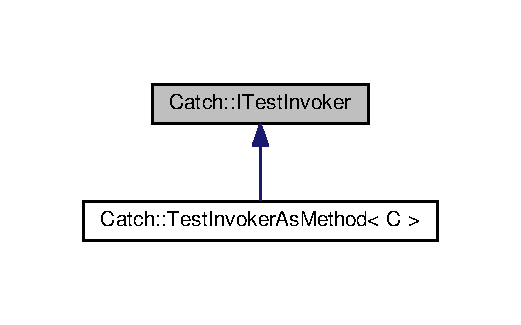
\includegraphics[width=250pt]{structCatch_1_1ITestInvoker__inherit__graph}
\end{center}
\end{figure}
\subsection*{Public Member Functions}
\begin{DoxyCompactItemize}
\item 
virtual void {\bfseries invoke} () const =0\hypertarget{structCatch_1_1ITestInvoker_a6fcd5c5b67d6d5ade6491ff33411ca7f}{}\label{structCatch_1_1ITestInvoker_a6fcd5c5b67d6d5ade6491ff33411ca7f}

\end{DoxyCompactItemize}


The documentation for this struct was generated from the following file\+:\begin{DoxyCompactItemize}
\item 
include/catch.\+hpp\end{DoxyCompactItemize}

\hypertarget{structCatch_1_1ITransientExpression}{}\section{Catch\+:\+:I\+Transient\+Expression Struct Reference}
\label{structCatch_1_1ITransientExpression}\index{Catch\+::\+I\+Transient\+Expression@{Catch\+::\+I\+Transient\+Expression}}


Inheritance diagram for Catch\+:\+:I\+Transient\+Expression\+:
\nopagebreak
\begin{figure}[H]
\begin{center}
\leavevmode
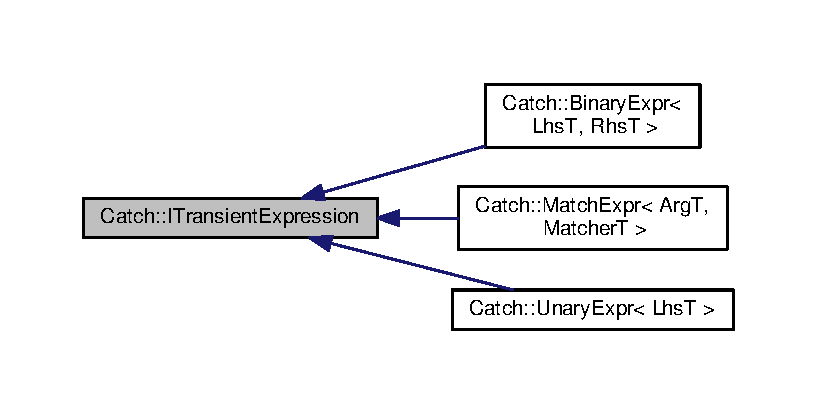
\includegraphics[width=350pt]{structCatch_1_1ITransientExpression__inherit__graph}
\end{center}
\end{figure}
\subsection*{Public Member Functions}
\begin{DoxyCompactItemize}
\item 
auto {\bfseries is\+Binary\+Expression} () const -\/$>$ bool\hypertarget{structCatch_1_1ITransientExpression_a3b436e13a0a6d3522bbf70d4e31deb22}{}\label{structCatch_1_1ITransientExpression_a3b436e13a0a6d3522bbf70d4e31deb22}

\item 
auto {\bfseries get\+Result} () const -\/$>$ bool\hypertarget{structCatch_1_1ITransientExpression_a101c7db86c87eff93a8ff496720e6320}{}\label{structCatch_1_1ITransientExpression_a101c7db86c87eff93a8ff496720e6320}

\item 
virtual void {\bfseries stream\+Reconstructed\+Expression} (std\+::ostream \&os) const =0\hypertarget{structCatch_1_1ITransientExpression_aabe1889df9c6e639a24afb08d8a0fe9e}{}\label{structCatch_1_1ITransientExpression_aabe1889df9c6e639a24afb08d8a0fe9e}

\item 
{\bfseries I\+Transient\+Expression} (bool is\+Binary\+Expression, bool result)\hypertarget{structCatch_1_1ITransientExpression_aafe69572b7ed884e63ec81f58d4afd8c}{}\label{structCatch_1_1ITransientExpression_aafe69572b7ed884e63ec81f58d4afd8c}

\end{DoxyCompactItemize}
\subsection*{Public Attributes}
\begin{DoxyCompactItemize}
\item 
bool {\bfseries m\+\_\+is\+Binary\+Expression}\hypertarget{structCatch_1_1ITransientExpression_a75ce48da824d514d08152d396abb28d8}{}\label{structCatch_1_1ITransientExpression_a75ce48da824d514d08152d396abb28d8}

\item 
bool {\bfseries m\+\_\+result}\hypertarget{structCatch_1_1ITransientExpression_a4646e2b5e0156e913653ec3b9b60c942}{}\label{structCatch_1_1ITransientExpression_a4646e2b5e0156e913653ec3b9b60c942}

\end{DoxyCompactItemize}


The documentation for this struct was generated from the following file\+:\begin{DoxyCompactItemize}
\item 
include/catch.\+hpp\end{DoxyCompactItemize}

\hypertarget{classCatch_1_1LazyExpression}{}\section{Catch\+:\+:Lazy\+Expression Class Reference}
\label{classCatch_1_1LazyExpression}\index{Catch\+::\+Lazy\+Expression@{Catch\+::\+Lazy\+Expression}}
\subsection*{Public Member Functions}
\begin{DoxyCompactItemize}
\item 
{\bfseries Lazy\+Expression} (bool is\+Negated)\hypertarget{classCatch_1_1LazyExpression_a47186c2487bd4bf871e870ba8048553a}{}\label{classCatch_1_1LazyExpression_a47186c2487bd4bf871e870ba8048553a}

\item 
{\bfseries Lazy\+Expression} (\hyperlink{classCatch_1_1LazyExpression}{Lazy\+Expression} const \&other)\hypertarget{classCatch_1_1LazyExpression_ab82d5e94df0e159b018fbde0170e46f8}{}\label{classCatch_1_1LazyExpression_ab82d5e94df0e159b018fbde0170e46f8}

\item 
\hyperlink{classCatch_1_1LazyExpression}{Lazy\+Expression} \& {\bfseries operator=} (\hyperlink{classCatch_1_1LazyExpression}{Lazy\+Expression} const \&)=delete\hypertarget{classCatch_1_1LazyExpression_ae4ae00d4f36f084c369f2da36565a822}{}\label{classCatch_1_1LazyExpression_ae4ae00d4f36f084c369f2da36565a822}

\item 
{\bfseries operator bool} () const \hypertarget{classCatch_1_1LazyExpression_a5f3541ec933ad977b6a10ddf61b45adc}{}\label{classCatch_1_1LazyExpression_a5f3541ec933ad977b6a10ddf61b45adc}

\end{DoxyCompactItemize}
\subsection*{Friends}
\begin{DoxyCompactItemize}
\item 
class {\bfseries Assertion\+Handler}\hypertarget{classCatch_1_1LazyExpression_a4301a3aa57b612dd8b6ef8461742ecab}{}\label{classCatch_1_1LazyExpression_a4301a3aa57b612dd8b6ef8461742ecab}

\item 
struct {\bfseries Assertion\+Stats}\hypertarget{classCatch_1_1LazyExpression_a64019eb137f5ce447cdc71cb80b6e7a4}{}\label{classCatch_1_1LazyExpression_a64019eb137f5ce447cdc71cb80b6e7a4}

\item 
class {\bfseries Run\+Context}\hypertarget{classCatch_1_1LazyExpression_af3aa096bb29a772bc534830f29a2ce7a}{}\label{classCatch_1_1LazyExpression_af3aa096bb29a772bc534830f29a2ce7a}

\item 
auto {\bfseries operator$<$$<$} (std\+::ostream \&os, \hyperlink{classCatch_1_1LazyExpression}{Lazy\+Expression} const \&lazy\+Expr) -\/$>$ std\+::ostream \&\hypertarget{classCatch_1_1LazyExpression_aa01086581cab2fcd2d4580b8fa787dfc}{}\label{classCatch_1_1LazyExpression_aa01086581cab2fcd2d4580b8fa787dfc}

\end{DoxyCompactItemize}


The documentation for this class was generated from the following file\+:\begin{DoxyCompactItemize}
\item 
include/catch.\+hpp\end{DoxyCompactItemize}

\hypertarget{structCatch_1_1Matchers_1_1Impl_1_1MatchAllOf}{}\section{Catch\+:\+:Matchers\+:\+:Impl\+:\+:Match\+All\+Of$<$ ArgT $>$ Struct Template Reference}
\label{structCatch_1_1Matchers_1_1Impl_1_1MatchAllOf}\index{Catch\+::\+Matchers\+::\+Impl\+::\+Match\+All\+Of$<$ Arg\+T $>$@{Catch\+::\+Matchers\+::\+Impl\+::\+Match\+All\+Of$<$ Arg\+T $>$}}


Inheritance diagram for Catch\+:\+:Matchers\+:\+:Impl\+:\+:Match\+All\+Of$<$ ArgT $>$\+:
\nopagebreak
\begin{figure}[H]
\begin{center}
\leavevmode
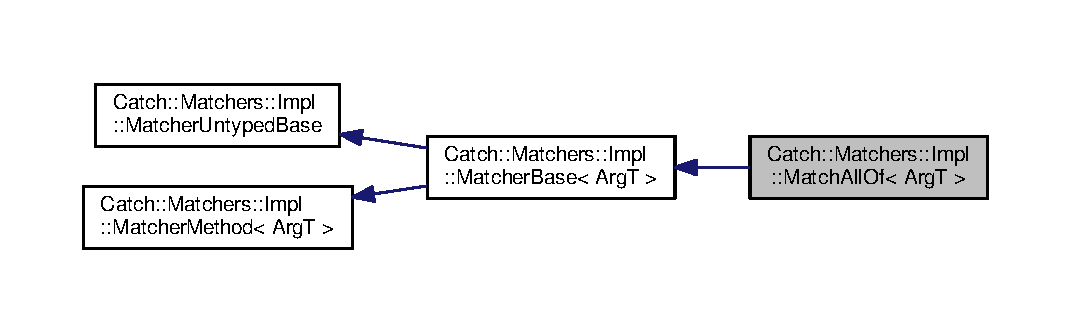
\includegraphics[width=350pt]{structCatch_1_1Matchers_1_1Impl_1_1MatchAllOf__inherit__graph}
\end{center}
\end{figure}


Collaboration diagram for Catch\+:\+:Matchers\+:\+:Impl\+:\+:Match\+All\+Of$<$ ArgT $>$\+:
\nopagebreak
\begin{figure}[H]
\begin{center}
\leavevmode
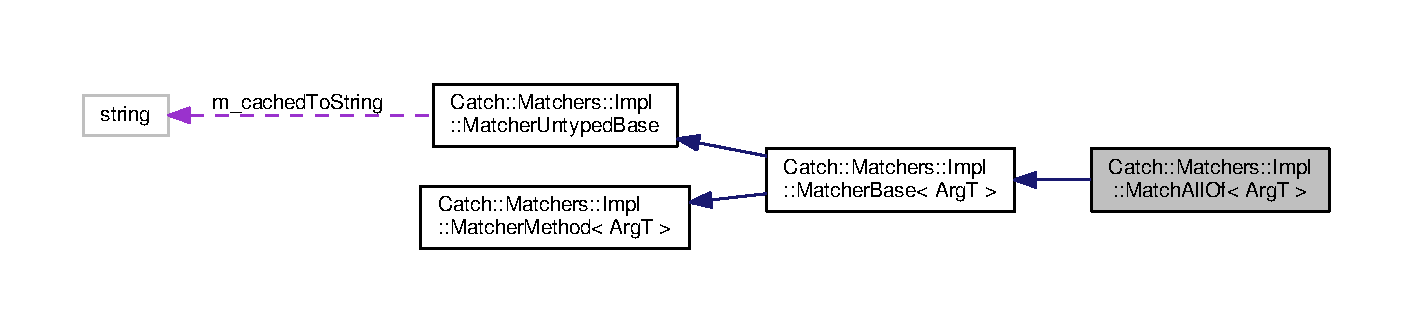
\includegraphics[width=350pt]{structCatch_1_1Matchers_1_1Impl_1_1MatchAllOf__coll__graph}
\end{center}
\end{figure}
\subsection*{Public Member Functions}
\begin{DoxyCompactItemize}
\item 
bool {\bfseries match} (ArgT const \&arg) const override\hypertarget{structCatch_1_1Matchers_1_1Impl_1_1MatchAllOf_acfb377bda2c58ae62e6df9c3a8a89f8f}{}\label{structCatch_1_1Matchers_1_1Impl_1_1MatchAllOf_acfb377bda2c58ae62e6df9c3a8a89f8f}

\item 
std\+::string {\bfseries describe} () const override\hypertarget{structCatch_1_1Matchers_1_1Impl_1_1MatchAllOf_acbb9a083e93b546fd33c9235b644c40f}{}\label{structCatch_1_1Matchers_1_1Impl_1_1MatchAllOf_acbb9a083e93b546fd33c9235b644c40f}

\item 
\hyperlink{structCatch_1_1Matchers_1_1Impl_1_1MatchAllOf}{Match\+All\+Of}$<$ ArgT $>$ \& {\bfseries operator\&\&} (\hyperlink{structCatch_1_1Matchers_1_1Impl_1_1MatcherBase}{Matcher\+Base}$<$ ArgT $>$ const \&other)\hypertarget{structCatch_1_1Matchers_1_1Impl_1_1MatchAllOf_a3844f9fb55f7a77155576ddc1e3f90d7}{}\label{structCatch_1_1Matchers_1_1Impl_1_1MatchAllOf_a3844f9fb55f7a77155576ddc1e3f90d7}

\end{DoxyCompactItemize}
\subsection*{Public Attributes}
\begin{DoxyCompactItemize}
\item 
std\+::vector$<$ \hyperlink{structCatch_1_1Matchers_1_1Impl_1_1MatcherBase}{Matcher\+Base}$<$ ArgT $>$ const $\ast$ $>$ {\bfseries m\+\_\+matchers}\hypertarget{structCatch_1_1Matchers_1_1Impl_1_1MatchAllOf_a98d6a2611f195a4a5c49f92fd877be9a}{}\label{structCatch_1_1Matchers_1_1Impl_1_1MatchAllOf_a98d6a2611f195a4a5c49f92fd877be9a}

\end{DoxyCompactItemize}
\subsection*{Additional Inherited Members}


The documentation for this struct was generated from the following file\+:\begin{DoxyCompactItemize}
\item 
include/catch.\+hpp\end{DoxyCompactItemize}

\hypertarget{structCatch_1_1Matchers_1_1Impl_1_1MatchAnyOf}{}\section{Catch\+:\+:Matchers\+:\+:Impl\+:\+:Match\+Any\+Of$<$ ArgT $>$ Struct Template Reference}
\label{structCatch_1_1Matchers_1_1Impl_1_1MatchAnyOf}\index{Catch\+::\+Matchers\+::\+Impl\+::\+Match\+Any\+Of$<$ Arg\+T $>$@{Catch\+::\+Matchers\+::\+Impl\+::\+Match\+Any\+Of$<$ Arg\+T $>$}}


Inheritance diagram for Catch\+:\+:Matchers\+:\+:Impl\+:\+:Match\+Any\+Of$<$ ArgT $>$\+:\nopagebreak
\begin{figure}[H]
\begin{center}
\leavevmode
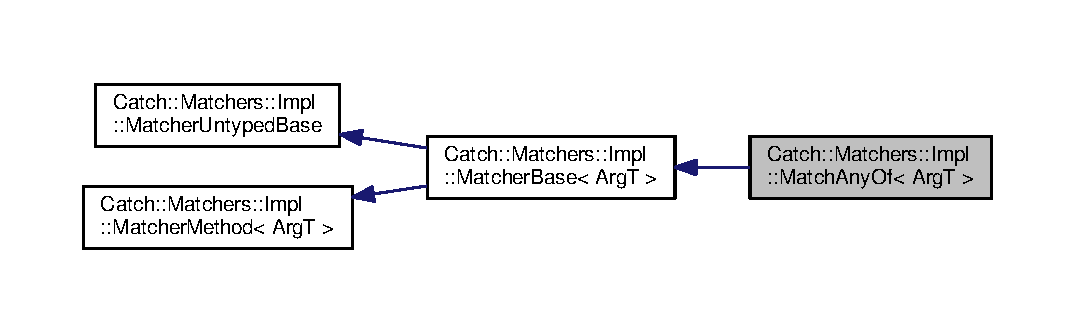
\includegraphics[width=350pt]{structCatch_1_1Matchers_1_1Impl_1_1MatchAnyOf__inherit__graph}
\end{center}
\end{figure}


Collaboration diagram for Catch\+:\+:Matchers\+:\+:Impl\+:\+:Match\+Any\+Of$<$ ArgT $>$\+:\nopagebreak
\begin{figure}[H]
\begin{center}
\leavevmode
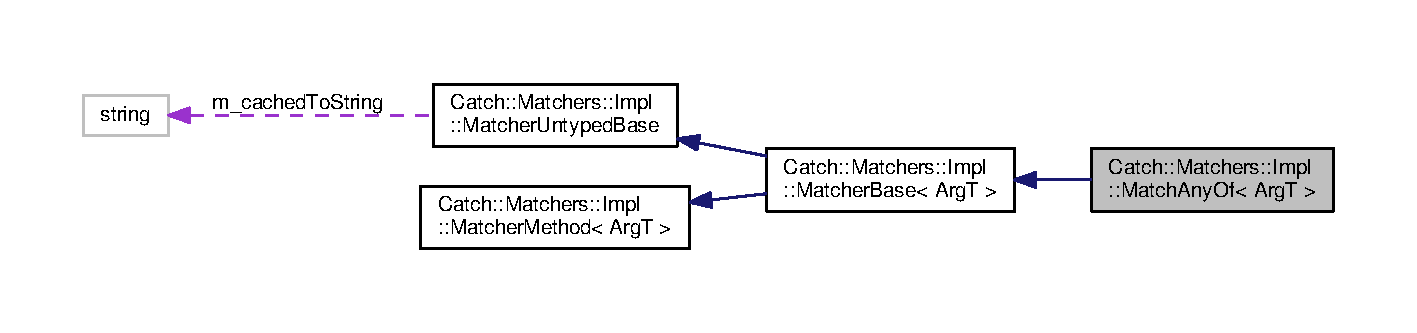
\includegraphics[width=350pt]{structCatch_1_1Matchers_1_1Impl_1_1MatchAnyOf__coll__graph}
\end{center}
\end{figure}
\subsection*{Public Member Functions}
\begin{DoxyCompactItemize}
\item 
bool {\bfseries match} (ArgT const \&arg) const override\hypertarget{structCatch_1_1Matchers_1_1Impl_1_1MatchAnyOf_a8a3e8338f979e56277dcf553efb78dc0}{}\label{structCatch_1_1Matchers_1_1Impl_1_1MatchAnyOf_a8a3e8338f979e56277dcf553efb78dc0}

\item 
std\+::string {\bfseries describe} () const override\hypertarget{structCatch_1_1Matchers_1_1Impl_1_1MatchAnyOf_a315285204df93d1f8e72f50dd66eb709}{}\label{structCatch_1_1Matchers_1_1Impl_1_1MatchAnyOf_a315285204df93d1f8e72f50dd66eb709}

\item 
\hyperlink{structCatch_1_1Matchers_1_1Impl_1_1MatchAnyOf}{Match\+Any\+Of}$<$ ArgT $>$ \& {\bfseries operator$\vert$$\vert$} (\hyperlink{structCatch_1_1Matchers_1_1Impl_1_1MatcherBase}{Matcher\+Base}$<$ ArgT $>$ const \&other)\hypertarget{structCatch_1_1Matchers_1_1Impl_1_1MatchAnyOf_a44d7582dbe09fc31b9a5ba8a6367b506}{}\label{structCatch_1_1Matchers_1_1Impl_1_1MatchAnyOf_a44d7582dbe09fc31b9a5ba8a6367b506}

\end{DoxyCompactItemize}
\subsection*{Public Attributes}
\begin{DoxyCompactItemize}
\item 
std\+::vector$<$ \hyperlink{structCatch_1_1Matchers_1_1Impl_1_1MatcherBase}{Matcher\+Base}$<$ ArgT $>$ const $\ast$ $>$ {\bfseries m\+\_\+matchers}\hypertarget{structCatch_1_1Matchers_1_1Impl_1_1MatchAnyOf_a1fb1119e6110dc15b8d5262ec0aeddd5}{}\label{structCatch_1_1Matchers_1_1Impl_1_1MatchAnyOf_a1fb1119e6110dc15b8d5262ec0aeddd5}

\end{DoxyCompactItemize}
\subsection*{Additional Inherited Members}


The documentation for this struct was generated from the following file\+:\begin{DoxyCompactItemize}
\item 
include/catch.\+hpp\end{DoxyCompactItemize}

\hypertarget{structCatch_1_1Matchers_1_1Impl_1_1MatcherBase}{}\section{Catch\+:\+:Matchers\+:\+:Impl\+:\+:Matcher\+Base$<$ T $>$ Struct Template Reference}
\label{structCatch_1_1Matchers_1_1Impl_1_1MatcherBase}\index{Catch\+::\+Matchers\+::\+Impl\+::\+Matcher\+Base$<$ T $>$@{Catch\+::\+Matchers\+::\+Impl\+::\+Matcher\+Base$<$ T $>$}}


Inheritance diagram for Catch\+:\+:Matchers\+:\+:Impl\+:\+:Matcher\+Base$<$ T $>$\+:\nopagebreak
\begin{figure}[H]
\begin{center}
\leavevmode
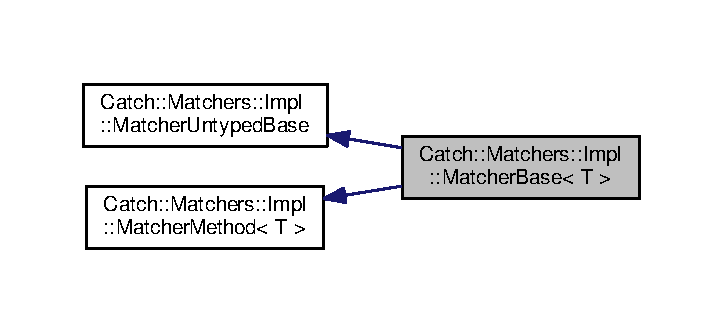
\includegraphics[width=347pt]{structCatch_1_1Matchers_1_1Impl_1_1MatcherBase__inherit__graph}
\end{center}
\end{figure}


Collaboration diagram for Catch\+:\+:Matchers\+:\+:Impl\+:\+:Matcher\+Base$<$ T $>$\+:\nopagebreak
\begin{figure}[H]
\begin{center}
\leavevmode
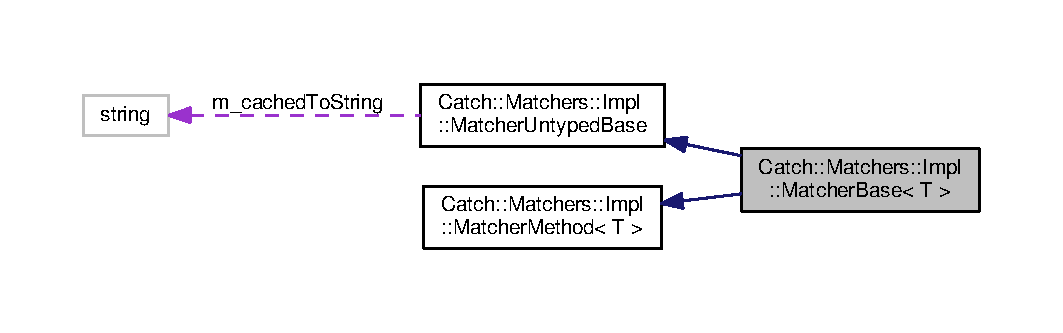
\includegraphics[width=350pt]{structCatch_1_1Matchers_1_1Impl_1_1MatcherBase__coll__graph}
\end{center}
\end{figure}
\subsection*{Public Member Functions}
\begin{DoxyCompactItemize}
\item 
\hyperlink{structCatch_1_1Matchers_1_1Impl_1_1MatchAllOf}{Match\+All\+Of}$<$ T $>$ {\bfseries operator\&\&} (\hyperlink{structCatch_1_1Matchers_1_1Impl_1_1MatcherBase}{Matcher\+Base} const \&other) const \hypertarget{structCatch_1_1Matchers_1_1Impl_1_1MatcherBase_a275a18e3e1c4d0bddfde34e362f66b6c}{}\label{structCatch_1_1Matchers_1_1Impl_1_1MatcherBase_a275a18e3e1c4d0bddfde34e362f66b6c}

\item 
\hyperlink{structCatch_1_1Matchers_1_1Impl_1_1MatchAnyOf}{Match\+Any\+Of}$<$ T $>$ {\bfseries operator$\vert$$\vert$} (\hyperlink{structCatch_1_1Matchers_1_1Impl_1_1MatcherBase}{Matcher\+Base} const \&other) const \hypertarget{structCatch_1_1Matchers_1_1Impl_1_1MatcherBase_a382ffd0d07d6a5cdadd2bd36ade0a742}{}\label{structCatch_1_1Matchers_1_1Impl_1_1MatcherBase_a382ffd0d07d6a5cdadd2bd36ade0a742}

\item 
\hyperlink{structCatch_1_1Matchers_1_1Impl_1_1MatchNotOf}{Match\+Not\+Of}$<$ T $>$ {\bfseries operator!} () const \hypertarget{structCatch_1_1Matchers_1_1Impl_1_1MatcherBase_afd5c25339eab93d9ea037fa4282fca7c}{}\label{structCatch_1_1Matchers_1_1Impl_1_1MatcherBase_afd5c25339eab93d9ea037fa4282fca7c}

\end{DoxyCompactItemize}
\subsection*{Additional Inherited Members}


The documentation for this struct was generated from the following file\+:\begin{DoxyCompactItemize}
\item 
include/catch.\+hpp\end{DoxyCompactItemize}

\hypertarget{structCatch_1_1Matchers_1_1Impl_1_1MatcherMethod}{}\section{Catch\+:\+:Matchers\+:\+:Impl\+:\+:Matcher\+Method$<$ ObjectT $>$ Struct Template Reference}
\label{structCatch_1_1Matchers_1_1Impl_1_1MatcherMethod}\index{Catch\+::\+Matchers\+::\+Impl\+::\+Matcher\+Method$<$ Object\+T $>$@{Catch\+::\+Matchers\+::\+Impl\+::\+Matcher\+Method$<$ Object\+T $>$}}
\subsection*{Public Member Functions}
\begin{DoxyCompactItemize}
\item 
virtual bool {\bfseries match} (ObjectT const \&arg) const =0\hypertarget{structCatch_1_1Matchers_1_1Impl_1_1MatcherMethod_ae0920ff9e817acf08e1bb0cbcb044e30}{}\label{structCatch_1_1Matchers_1_1Impl_1_1MatcherMethod_ae0920ff9e817acf08e1bb0cbcb044e30}

\end{DoxyCompactItemize}


The documentation for this struct was generated from the following file\+:\begin{DoxyCompactItemize}
\item 
include/catch.\+hpp\end{DoxyCompactItemize}

\hypertarget{structCatch_1_1Matchers_1_1Impl_1_1MatcherMethod_3_01PtrT_01_5_01_4}{}\section{Catch\+:\+:Matchers\+:\+:Impl\+:\+:Matcher\+Method$<$ PtrT $\ast$ $>$ Struct Template Reference}
\label{structCatch_1_1Matchers_1_1Impl_1_1MatcherMethod_3_01PtrT_01_5_01_4}\index{Catch\+::\+Matchers\+::\+Impl\+::\+Matcher\+Method$<$ Ptr\+T $\ast$ $>$@{Catch\+::\+Matchers\+::\+Impl\+::\+Matcher\+Method$<$ Ptr\+T $\ast$ $>$}}
\subsection*{Public Member Functions}
\begin{DoxyCompactItemize}
\item 
virtual bool {\bfseries match} (PtrT $\ast$arg) const =0\hypertarget{structCatch_1_1Matchers_1_1Impl_1_1MatcherMethod_3_01PtrT_01_5_01_4_a5fdd64f9509724f32ffc73cb320181d1}{}\label{structCatch_1_1Matchers_1_1Impl_1_1MatcherMethod_3_01PtrT_01_5_01_4_a5fdd64f9509724f32ffc73cb320181d1}

\end{DoxyCompactItemize}


The documentation for this struct was generated from the following file\+:\begin{DoxyCompactItemize}
\item 
include/catch.\+hpp\end{DoxyCompactItemize}

\hypertarget{classCatch_1_1Matchers_1_1Impl_1_1MatcherUntypedBase}{}\section{Catch\+:\+:Matchers\+:\+:Impl\+:\+:Matcher\+Untyped\+Base Class Reference}
\label{classCatch_1_1Matchers_1_1Impl_1_1MatcherUntypedBase}\index{Catch\+::\+Matchers\+::\+Impl\+::\+Matcher\+Untyped\+Base@{Catch\+::\+Matchers\+::\+Impl\+::\+Matcher\+Untyped\+Base}}


Inheritance diagram for Catch\+:\+:Matchers\+:\+:Impl\+:\+:Matcher\+Untyped\+Base\+:\nopagebreak
\begin{figure}[H]
\begin{center}
\leavevmode
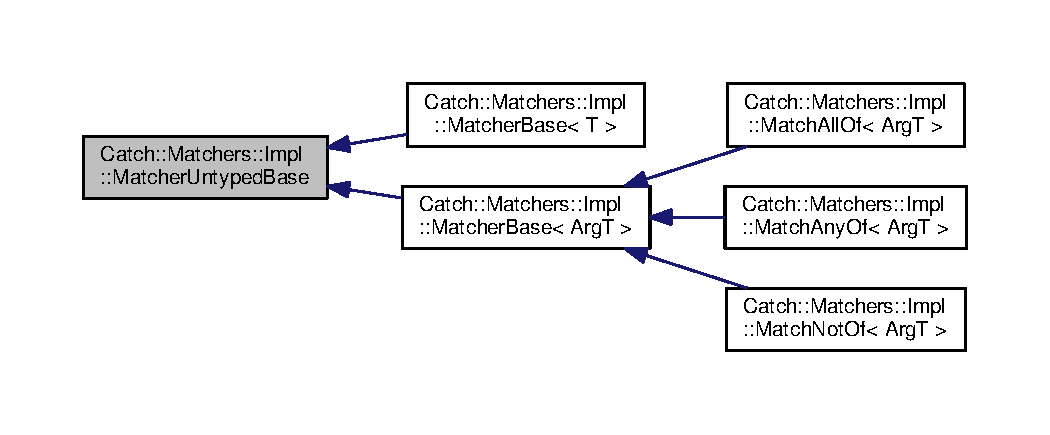
\includegraphics[width=350pt]{classCatch_1_1Matchers_1_1Impl_1_1MatcherUntypedBase__inherit__graph}
\end{center}
\end{figure}


Collaboration diagram for Catch\+:\+:Matchers\+:\+:Impl\+:\+:Matcher\+Untyped\+Base\+:\nopagebreak
\begin{figure}[H]
\begin{center}
\leavevmode
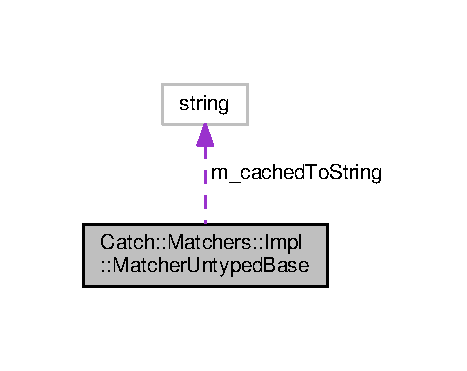
\includegraphics[width=224pt]{classCatch_1_1Matchers_1_1Impl_1_1MatcherUntypedBase__coll__graph}
\end{center}
\end{figure}
\subsection*{Public Member Functions}
\begin{DoxyCompactItemize}
\item 
{\bfseries Matcher\+Untyped\+Base} (\hyperlink{classCatch_1_1Matchers_1_1Impl_1_1MatcherUntypedBase}{Matcher\+Untyped\+Base} const \&)=default\hypertarget{classCatch_1_1Matchers_1_1Impl_1_1MatcherUntypedBase_a985fd3c3ffcc9f2e8dc7a330130040b0}{}\label{classCatch_1_1Matchers_1_1Impl_1_1MatcherUntypedBase_a985fd3c3ffcc9f2e8dc7a330130040b0}

\item 
\hyperlink{classCatch_1_1Matchers_1_1Impl_1_1MatcherUntypedBase}{Matcher\+Untyped\+Base} \& {\bfseries operator=} (\hyperlink{classCatch_1_1Matchers_1_1Impl_1_1MatcherUntypedBase}{Matcher\+Untyped\+Base} const \&)=delete\hypertarget{classCatch_1_1Matchers_1_1Impl_1_1MatcherUntypedBase_a62668ccc47b64a9094dcb6413f9af80b}{}\label{classCatch_1_1Matchers_1_1Impl_1_1MatcherUntypedBase_a62668ccc47b64a9094dcb6413f9af80b}

\item 
std\+::string {\bfseries to\+String} () const \hypertarget{classCatch_1_1Matchers_1_1Impl_1_1MatcherUntypedBase_a9667f989b08e52a1ce96c955456db8f9}{}\label{classCatch_1_1Matchers_1_1Impl_1_1MatcherUntypedBase_a9667f989b08e52a1ce96c955456db8f9}

\end{DoxyCompactItemize}
\subsection*{Protected Member Functions}
\begin{DoxyCompactItemize}
\item 
virtual std\+::string {\bfseries describe} () const =0\hypertarget{classCatch_1_1Matchers_1_1Impl_1_1MatcherUntypedBase_a91d3a907dbfcbb596077df24f6e11fe2}{}\label{classCatch_1_1Matchers_1_1Impl_1_1MatcherUntypedBase_a91d3a907dbfcbb596077df24f6e11fe2}

\end{DoxyCompactItemize}
\subsection*{Protected Attributes}
\begin{DoxyCompactItemize}
\item 
std\+::string {\bfseries m\+\_\+cached\+To\+String}\hypertarget{classCatch_1_1Matchers_1_1Impl_1_1MatcherUntypedBase_a951095c462657e7097a9a6dc4dde813f}{}\label{classCatch_1_1Matchers_1_1Impl_1_1MatcherUntypedBase_a951095c462657e7097a9a6dc4dde813f}

\end{DoxyCompactItemize}


The documentation for this class was generated from the following file\+:\begin{DoxyCompactItemize}
\item 
include/catch.\+hpp\end{DoxyCompactItemize}

\hypertarget{classCatch_1_1MatchExpr}{}\section{Catch\+:\+:Match\+Expr$<$ ArgT, MatcherT $>$ Class Template Reference}
\label{classCatch_1_1MatchExpr}\index{Catch\+::\+Match\+Expr$<$ Arg\+T, Matcher\+T $>$@{Catch\+::\+Match\+Expr$<$ Arg\+T, Matcher\+T $>$}}


Inheritance diagram for Catch\+:\+:Match\+Expr$<$ ArgT, MatcherT $>$\+:\nopagebreak
\begin{figure}[H]
\begin{center}
\leavevmode
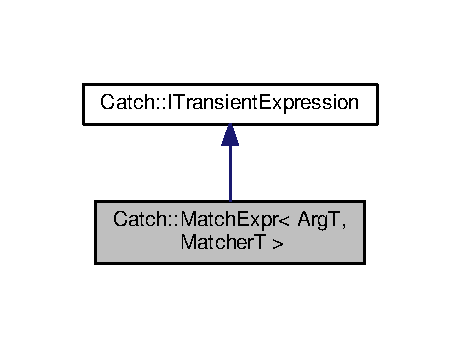
\includegraphics[width=221pt]{classCatch_1_1MatchExpr__inherit__graph}
\end{center}
\end{figure}


Collaboration diagram for Catch\+:\+:Match\+Expr$<$ ArgT, MatcherT $>$\+:\nopagebreak
\begin{figure}[H]
\begin{center}
\leavevmode
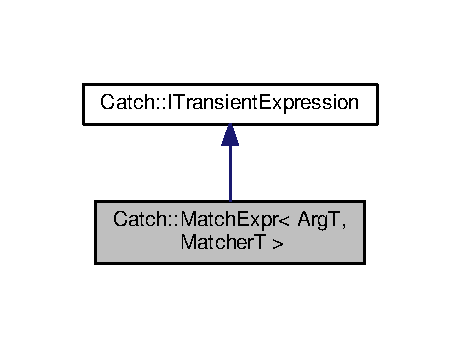
\includegraphics[width=221pt]{classCatch_1_1MatchExpr__coll__graph}
\end{center}
\end{figure}
\subsection*{Public Member Functions}
\begin{DoxyCompactItemize}
\item 
{\bfseries Match\+Expr} (ArgT const \&arg, MatcherT const \&matcher, \hyperlink{classCatch_1_1StringRef}{String\+Ref} matcher\+String)\hypertarget{classCatch_1_1MatchExpr_ab5b9ecc4fb9e91f5f48756e75affe93d}{}\label{classCatch_1_1MatchExpr_ab5b9ecc4fb9e91f5f48756e75affe93d}

\item 
void {\bfseries stream\+Reconstructed\+Expression} (std\+::ostream \&os) const override\hypertarget{classCatch_1_1MatchExpr_ad3e41adb597750b2219bb37e51185629}{}\label{classCatch_1_1MatchExpr_ad3e41adb597750b2219bb37e51185629}

\end{DoxyCompactItemize}
\subsection*{Additional Inherited Members}


The documentation for this class was generated from the following file\+:\begin{DoxyCompactItemize}
\item 
include/catch.\+hpp\end{DoxyCompactItemize}

\hypertarget{structCatch_1_1Matchers_1_1Impl_1_1MatchNotOf}{}\section{Catch\+:\+:Matchers\+:\+:Impl\+:\+:Match\+Not\+Of$<$ ArgT $>$ Struct Template Reference}
\label{structCatch_1_1Matchers_1_1Impl_1_1MatchNotOf}\index{Catch\+::\+Matchers\+::\+Impl\+::\+Match\+Not\+Of$<$ Arg\+T $>$@{Catch\+::\+Matchers\+::\+Impl\+::\+Match\+Not\+Of$<$ Arg\+T $>$}}


Inheritance diagram for Catch\+:\+:Matchers\+:\+:Impl\+:\+:Match\+Not\+Of$<$ ArgT $>$\+:\nopagebreak
\begin{figure}[H]
\begin{center}
\leavevmode
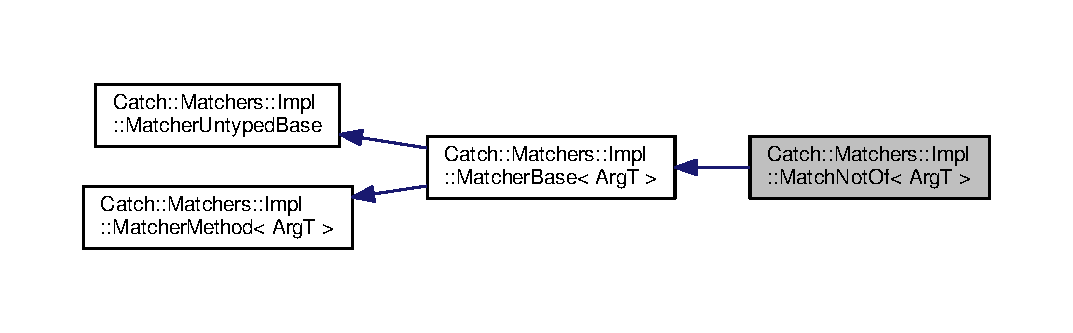
\includegraphics[width=350pt]{structCatch_1_1Matchers_1_1Impl_1_1MatchNotOf__inherit__graph}
\end{center}
\end{figure}


Collaboration diagram for Catch\+:\+:Matchers\+:\+:Impl\+:\+:Match\+Not\+Of$<$ ArgT $>$\+:\nopagebreak
\begin{figure}[H]
\begin{center}
\leavevmode
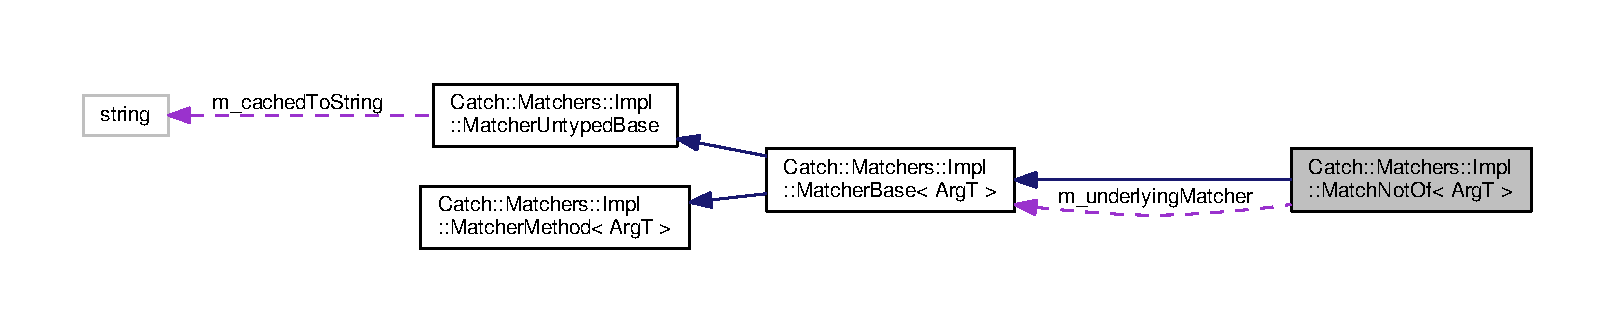
\includegraphics[width=350pt]{structCatch_1_1Matchers_1_1Impl_1_1MatchNotOf__coll__graph}
\end{center}
\end{figure}
\subsection*{Public Member Functions}
\begin{DoxyCompactItemize}
\item 
{\bfseries Match\+Not\+Of} (\hyperlink{structCatch_1_1Matchers_1_1Impl_1_1MatcherBase}{Matcher\+Base}$<$ ArgT $>$ const \&underlying\+Matcher)\hypertarget{structCatch_1_1Matchers_1_1Impl_1_1MatchNotOf_a47afdd9e4c3354cef85adc3186097ae4}{}\label{structCatch_1_1Matchers_1_1Impl_1_1MatchNotOf_a47afdd9e4c3354cef85adc3186097ae4}

\item 
bool {\bfseries match} (ArgT const \&arg) const override\hypertarget{structCatch_1_1Matchers_1_1Impl_1_1MatchNotOf_a181d693c0258e582d80dc6117a1f2b66}{}\label{structCatch_1_1Matchers_1_1Impl_1_1MatchNotOf_a181d693c0258e582d80dc6117a1f2b66}

\item 
std\+::string {\bfseries describe} () const override\hypertarget{structCatch_1_1Matchers_1_1Impl_1_1MatchNotOf_ac5fb4ef6a9069d23a4098c3c818f06b0}{}\label{structCatch_1_1Matchers_1_1Impl_1_1MatchNotOf_ac5fb4ef6a9069d23a4098c3c818f06b0}

\end{DoxyCompactItemize}
\subsection*{Public Attributes}
\begin{DoxyCompactItemize}
\item 
\hyperlink{structCatch_1_1Matchers_1_1Impl_1_1MatcherBase}{Matcher\+Base}$<$ ArgT $>$ const \& {\bfseries m\+\_\+underlying\+Matcher}\hypertarget{structCatch_1_1Matchers_1_1Impl_1_1MatchNotOf_af7ac67f112b0e93796b048a47329aad4}{}\label{structCatch_1_1Matchers_1_1Impl_1_1MatchNotOf_af7ac67f112b0e93796b048a47329aad4}

\end{DoxyCompactItemize}
\subsection*{Additional Inherited Members}


The documentation for this struct was generated from the following file\+:\begin{DoxyCompactItemize}
\item 
include/catch.\+hpp\end{DoxyCompactItemize}

\hypertarget{structCatch_1_1MessageBuilder}{}\section{Catch\+:\+:Message\+Builder Struct Reference}
\label{structCatch_1_1MessageBuilder}\index{Catch\+::\+Message\+Builder@{Catch\+::\+Message\+Builder}}


Inheritance diagram for Catch\+:\+:Message\+Builder\+:
\nopagebreak
\begin{figure}[H]
\begin{center}
\leavevmode
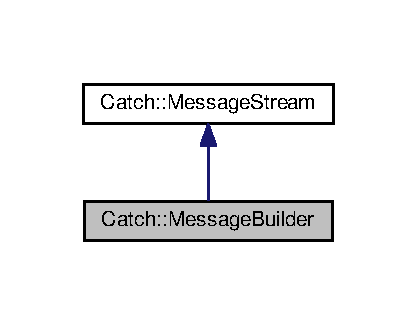
\includegraphics[width=200pt]{structCatch_1_1MessageBuilder__inherit__graph}
\end{center}
\end{figure}


Collaboration diagram for Catch\+:\+:Message\+Builder\+:
\nopagebreak
\begin{figure}[H]
\begin{center}
\leavevmode
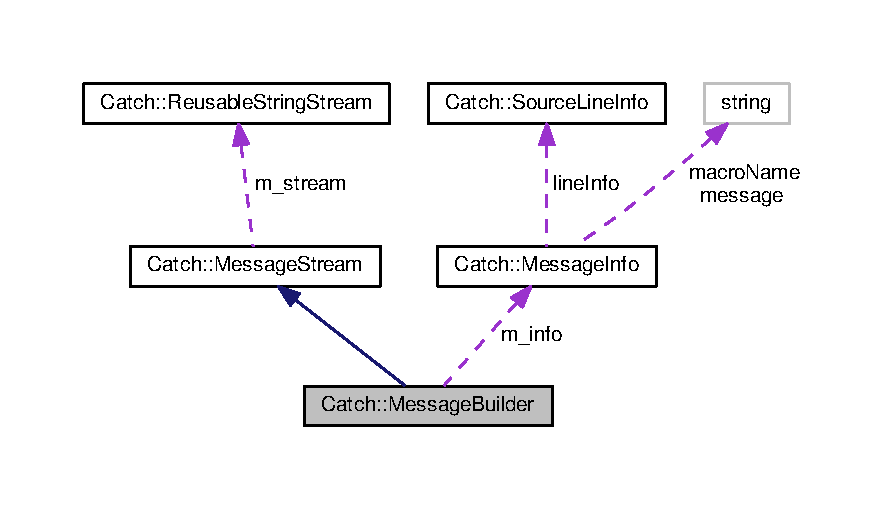
\includegraphics[width=350pt]{structCatch_1_1MessageBuilder__coll__graph}
\end{center}
\end{figure}
\subsection*{Public Member Functions}
\begin{DoxyCompactItemize}
\item 
{\bfseries Message\+Builder} (std\+::string const \&macro\+Name, \hyperlink{structCatch_1_1SourceLineInfo}{Source\+Line\+Info} const \&line\+Info, Result\+Was\+::\+Of\+Type type)\hypertarget{structCatch_1_1MessageBuilder_ab0c6378e722680bf58852c6ee2b6e724}{}\label{structCatch_1_1MessageBuilder_ab0c6378e722680bf58852c6ee2b6e724}

\item 
{\footnotesize template$<$typename T $>$ }\\\hyperlink{structCatch_1_1MessageBuilder}{Message\+Builder} \& {\bfseries operator$<$$<$} (T const \&value)\hypertarget{structCatch_1_1MessageBuilder_a20fa48d069b20dddcc2d3df8abb123c1}{}\label{structCatch_1_1MessageBuilder_a20fa48d069b20dddcc2d3df8abb123c1}

\end{DoxyCompactItemize}
\subsection*{Public Attributes}
\begin{DoxyCompactItemize}
\item 
\hyperlink{structCatch_1_1MessageInfo}{Message\+Info} {\bfseries m\+\_\+info}\hypertarget{structCatch_1_1MessageBuilder_a979f1c2b36d78f80ee275bfa5ba0209f}{}\label{structCatch_1_1MessageBuilder_a979f1c2b36d78f80ee275bfa5ba0209f}

\end{DoxyCompactItemize}


The documentation for this struct was generated from the following file\+:\begin{DoxyCompactItemize}
\item 
include/catch.\+hpp\end{DoxyCompactItemize}

\hypertarget{structCatch_1_1MessageInfo}{}\section{Catch\+:\+:Message\+Info Struct Reference}
\label{structCatch_1_1MessageInfo}\index{Catch\+::\+Message\+Info@{Catch\+::\+Message\+Info}}


Collaboration diagram for Catch\+:\+:Message\+Info\+:\nopagebreak
\begin{figure}[H]
\begin{center}
\leavevmode
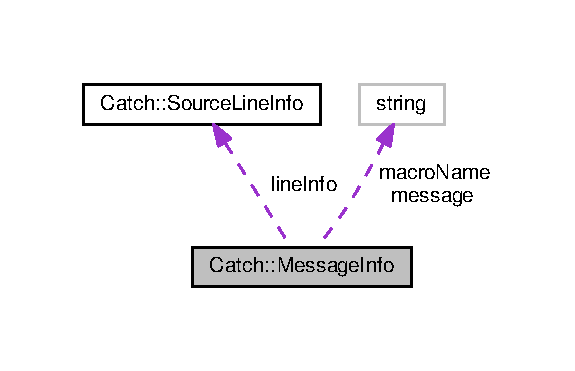
\includegraphics[width=276pt]{structCatch_1_1MessageInfo__coll__graph}
\end{center}
\end{figure}
\subsection*{Public Member Functions}
\begin{DoxyCompactItemize}
\item 
{\bfseries Message\+Info} (std\+::string const \&\+\_\+macro\+Name, \hyperlink{structCatch_1_1SourceLineInfo}{Source\+Line\+Info} const \&\+\_\+line\+Info, Result\+Was\+::\+Of\+Type \+\_\+type)\hypertarget{structCatch_1_1MessageInfo_a2e336c33ebef7af3c1bbae6a56e14f8a}{}\label{structCatch_1_1MessageInfo_a2e336c33ebef7af3c1bbae6a56e14f8a}

\item 
bool {\bfseries operator==} (\hyperlink{structCatch_1_1MessageInfo}{Message\+Info} const \&other) const \hypertarget{structCatch_1_1MessageInfo_a30fe117138e568c5a9dfdabb7de6e790}{}\label{structCatch_1_1MessageInfo_a30fe117138e568c5a9dfdabb7de6e790}

\item 
bool {\bfseries operator$<$} (\hyperlink{structCatch_1_1MessageInfo}{Message\+Info} const \&other) const \hypertarget{structCatch_1_1MessageInfo_a7a2b1ec3772cd35176e2ee25a94be16a}{}\label{structCatch_1_1MessageInfo_a7a2b1ec3772cd35176e2ee25a94be16a}

\end{DoxyCompactItemize}
\subsection*{Public Attributes}
\begin{DoxyCompactItemize}
\item 
std\+::string {\bfseries macro\+Name}\hypertarget{structCatch_1_1MessageInfo_a156ade4b3cc731f6ec7b542ae47ba8e3}{}\label{structCatch_1_1MessageInfo_a156ade4b3cc731f6ec7b542ae47ba8e3}

\item 
std\+::string {\bfseries message}\hypertarget{structCatch_1_1MessageInfo_ab6cd06e050bf426c6577502a5c50e256}{}\label{structCatch_1_1MessageInfo_ab6cd06e050bf426c6577502a5c50e256}

\item 
\hyperlink{structCatch_1_1SourceLineInfo}{Source\+Line\+Info} {\bfseries line\+Info}\hypertarget{structCatch_1_1MessageInfo_a985165328723e599696ebd8e43195cc5}{}\label{structCatch_1_1MessageInfo_a985165328723e599696ebd8e43195cc5}

\item 
Result\+Was\+::\+Of\+Type {\bfseries type}\hypertarget{structCatch_1_1MessageInfo_ae928b9117465c696e45951d9d0284e78}{}\label{structCatch_1_1MessageInfo_ae928b9117465c696e45951d9d0284e78}

\item 
unsigned int {\bfseries sequence}\hypertarget{structCatch_1_1MessageInfo_a7f4f57ea21e50160adefce7b68a781d6}{}\label{structCatch_1_1MessageInfo_a7f4f57ea21e50160adefce7b68a781d6}

\end{DoxyCompactItemize}


The documentation for this struct was generated from the following file\+:\begin{DoxyCompactItemize}
\item 
include/catch.\+hpp\end{DoxyCompactItemize}

\hypertarget{structCatch_1_1MessageStream}{}\section{Catch\+:\+:Message\+Stream Struct Reference}
\label{structCatch_1_1MessageStream}\index{Catch\+::\+Message\+Stream@{Catch\+::\+Message\+Stream}}


Inheritance diagram for Catch\+:\+:Message\+Stream\+:\nopagebreak
\begin{figure}[H]
\begin{center}
\leavevmode
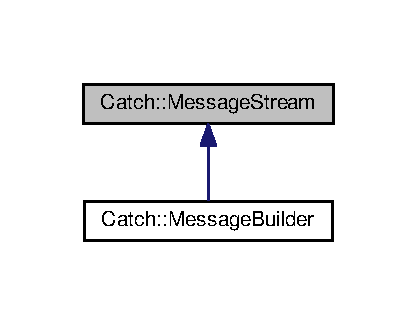
\includegraphics[width=200pt]{structCatch_1_1MessageStream__inherit__graph}
\end{center}
\end{figure}


Collaboration diagram for Catch\+:\+:Message\+Stream\+:\nopagebreak
\begin{figure}[H]
\begin{center}
\leavevmode
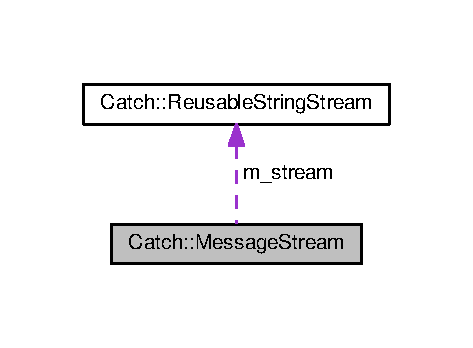
\includegraphics[width=227pt]{structCatch_1_1MessageStream__coll__graph}
\end{center}
\end{figure}
\subsection*{Public Member Functions}
\begin{DoxyCompactItemize}
\item 
{\footnotesize template$<$typename T $>$ }\\\hyperlink{structCatch_1_1MessageStream}{Message\+Stream} \& {\bfseries operator$<$$<$} (T const \&value)\hypertarget{structCatch_1_1MessageStream_a554c4aff5925a077e9fe9d858217428d}{}\label{structCatch_1_1MessageStream_a554c4aff5925a077e9fe9d858217428d}

\end{DoxyCompactItemize}
\subsection*{Public Attributes}
\begin{DoxyCompactItemize}
\item 
\hyperlink{classCatch_1_1ReusableStringStream}{Reusable\+String\+Stream} {\bfseries m\+\_\+stream}\hypertarget{structCatch_1_1MessageStream_a9202520faed8882ef469db9f353ec578}{}\label{structCatch_1_1MessageStream_a9202520faed8882ef469db9f353ec578}

\end{DoxyCompactItemize}


The documentation for this struct was generated from the following file\+:\begin{DoxyCompactItemize}
\item 
include/catch.\+hpp\end{DoxyCompactItemize}

\hypertarget{structCatch_1_1NameAndTags}{}\section{Catch\+:\+:Name\+And\+Tags Struct Reference}
\label{structCatch_1_1NameAndTags}\index{Catch\+::\+Name\+And\+Tags@{Catch\+::\+Name\+And\+Tags}}


Collaboration diagram for Catch\+:\+:Name\+And\+Tags\+:\nopagebreak
\begin{figure}[H]
\begin{center}
\leavevmode
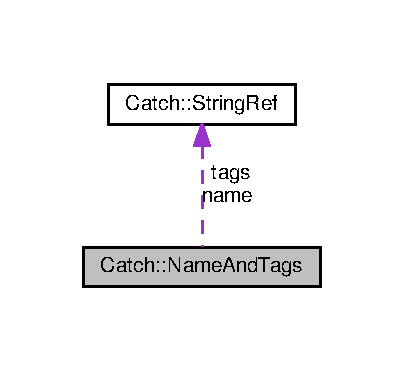
\includegraphics[width=194pt]{structCatch_1_1NameAndTags__coll__graph}
\end{center}
\end{figure}
\subsection*{Public Member Functions}
\begin{DoxyCompactItemize}
\item 
{\bfseries Name\+And\+Tags} (\hyperlink{classCatch_1_1StringRef}{String\+Ref} const \&name\+\_\+=\hyperlink{classCatch_1_1StringRef}{String\+Ref}(), \hyperlink{classCatch_1_1StringRef}{String\+Ref} const \&tags\+\_\+=\hyperlink{classCatch_1_1StringRef}{String\+Ref}()) noexcept\hypertarget{structCatch_1_1NameAndTags_ab585111e615ce8c504a2b9630de8ee94}{}\label{structCatch_1_1NameAndTags_ab585111e615ce8c504a2b9630de8ee94}

\end{DoxyCompactItemize}
\subsection*{Public Attributes}
\begin{DoxyCompactItemize}
\item 
\hyperlink{classCatch_1_1StringRef}{String\+Ref} {\bfseries name}\hypertarget{structCatch_1_1NameAndTags_a7cbea60e0cebfa622c667008eb011420}{}\label{structCatch_1_1NameAndTags_a7cbea60e0cebfa622c667008eb011420}

\item 
\hyperlink{classCatch_1_1StringRef}{String\+Ref} {\bfseries tags}\hypertarget{structCatch_1_1NameAndTags_a74062ed1138834a348424eb7ed900c57}{}\label{structCatch_1_1NameAndTags_a74062ed1138834a348424eb7ed900c57}

\end{DoxyCompactItemize}


The documentation for this struct was generated from the following file\+:\begin{DoxyCompactItemize}
\item 
include/catch.\+hpp\end{DoxyCompactItemize}

\hypertarget{classCatch_1_1NonCopyable}{}\section{Catch\+:\+:Non\+Copyable Class Reference}
\label{classCatch_1_1NonCopyable}\index{Catch\+::\+Non\+Copyable@{Catch\+::\+Non\+Copyable}}


Inheritance diagram for Catch\+:\+:Non\+Copyable\+:
\nopagebreak
\begin{figure}[H]
\begin{center}
\leavevmode
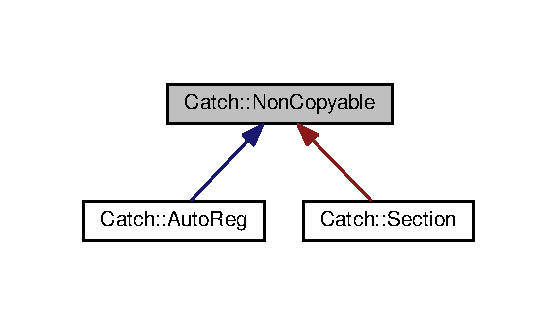
\includegraphics[width=268pt]{classCatch_1_1NonCopyable__inherit__graph}
\end{center}
\end{figure}


The documentation for this class was generated from the following file\+:\begin{DoxyCompactItemize}
\item 
include/catch.\+hpp\end{DoxyCompactItemize}

\hypertarget{structCatch_1_1not__this__one}{}\section{Catch\+:\+:not\+\_\+this\+\_\+one Struct Reference}
\label{structCatch_1_1not__this__one}\index{Catch\+::not\+\_\+this\+\_\+one@{Catch\+::not\+\_\+this\+\_\+one}}


The documentation for this struct was generated from the following file\+:\begin{DoxyCompactItemize}
\item 
include/catch.\+hpp\end{DoxyCompactItemize}

\hypertarget{structCatch_1_1pluralise}{}\section{Catch\+:\+:pluralise Struct Reference}
\label{structCatch_1_1pluralise}\index{Catch\+::pluralise@{Catch\+::pluralise}}


Collaboration diagram for Catch\+:\+:pluralise\+:\nopagebreak
\begin{figure}[H]
\begin{center}
\leavevmode
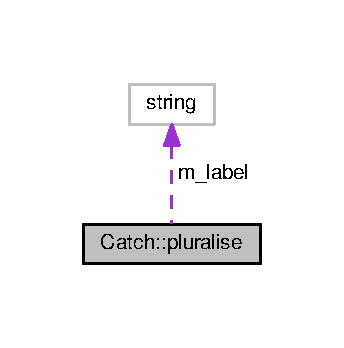
\includegraphics[width=165pt]{structCatch_1_1pluralise__coll__graph}
\end{center}
\end{figure}
\subsection*{Public Member Functions}
\begin{DoxyCompactItemize}
\item 
{\bfseries pluralise} (std\+::size\+\_\+t count, std\+::string const \&label)\hypertarget{structCatch_1_1pluralise_a5c55e22de2416cfe416edf715c6b9234}{}\label{structCatch_1_1pluralise_a5c55e22de2416cfe416edf715c6b9234}

\end{DoxyCompactItemize}
\subsection*{Public Attributes}
\begin{DoxyCompactItemize}
\item 
std\+::size\+\_\+t {\bfseries m\+\_\+count}\hypertarget{structCatch_1_1pluralise_a4dce2fa13ec6f00fac09b2418265441e}{}\label{structCatch_1_1pluralise_a4dce2fa13ec6f00fac09b2418265441e}

\item 
std\+::string {\bfseries m\+\_\+label}\hypertarget{structCatch_1_1pluralise_a8849cbdd3f11ebe7747597c8644e8793}{}\label{structCatch_1_1pluralise_a8849cbdd3f11ebe7747597c8644e8793}

\end{DoxyCompactItemize}
\subsection*{Friends}
\begin{DoxyCompactItemize}
\item 
std\+::ostream \& {\bfseries operator$<$$<$} (std\+::ostream \&os, \hyperlink{structCatch_1_1pluralise}{pluralise} const \&pluraliser)\hypertarget{structCatch_1_1pluralise_aa7dac6b165514c1f85e0695d678fdef5}{}\label{structCatch_1_1pluralise_aa7dac6b165514c1f85e0695d678fdef5}

\end{DoxyCompactItemize}


The documentation for this struct was generated from the following file\+:\begin{DoxyCompactItemize}
\item 
include/catch.\+hpp\end{DoxyCompactItemize}

\hypertarget{structCatch_1_1Matchers_1_1StdString_1_1RegexMatcher}{}\section{Catch\+:\+:Matchers\+:\+:Std\+String\+:\+:Regex\+Matcher Struct Reference}
\label{structCatch_1_1Matchers_1_1StdString_1_1RegexMatcher}\index{Catch\+::\+Matchers\+::\+Std\+String\+::\+Regex\+Matcher@{Catch\+::\+Matchers\+::\+Std\+String\+::\+Regex\+Matcher}}


Inheritance diagram for Catch\+:\+:Matchers\+:\+:Std\+String\+:\+:Regex\+Matcher\+:\nopagebreak
\begin{figure}[H]
\begin{center}
\leavevmode
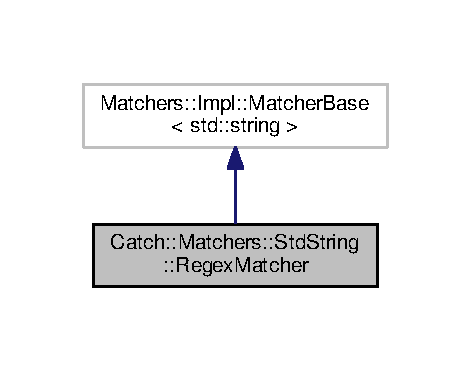
\includegraphics[width=226pt]{structCatch_1_1Matchers_1_1StdString_1_1RegexMatcher__inherit__graph}
\end{center}
\end{figure}


Collaboration diagram for Catch\+:\+:Matchers\+:\+:Std\+String\+:\+:Regex\+Matcher\+:\nopagebreak
\begin{figure}[H]
\begin{center}
\leavevmode
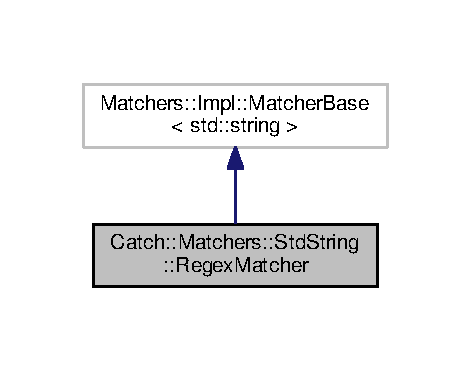
\includegraphics[width=226pt]{structCatch_1_1Matchers_1_1StdString_1_1RegexMatcher__coll__graph}
\end{center}
\end{figure}
\subsection*{Public Member Functions}
\begin{DoxyCompactItemize}
\item 
{\bfseries Regex\+Matcher} (std\+::string regex, Case\+Sensitive\+::\+Choice case\+Sensitivity)\hypertarget{structCatch_1_1Matchers_1_1StdString_1_1RegexMatcher_ab914deb885fe25558c41ab368c6b3916}{}\label{structCatch_1_1Matchers_1_1StdString_1_1RegexMatcher_ab914deb885fe25558c41ab368c6b3916}

\item 
bool {\bfseries match} (std\+::string const \&matchee) const override\hypertarget{structCatch_1_1Matchers_1_1StdString_1_1RegexMatcher_aa8e61adccabb2f36133029301f6b8f4e}{}\label{structCatch_1_1Matchers_1_1StdString_1_1RegexMatcher_aa8e61adccabb2f36133029301f6b8f4e}

\item 
std\+::string {\bfseries describe} () const override\hypertarget{structCatch_1_1Matchers_1_1StdString_1_1RegexMatcher_a1f788cd5258c987e5043f6c7f43adeb9}{}\label{structCatch_1_1Matchers_1_1StdString_1_1RegexMatcher_a1f788cd5258c987e5043f6c7f43adeb9}

\end{DoxyCompactItemize}


The documentation for this struct was generated from the following file\+:\begin{DoxyCompactItemize}
\item 
include/catch.\+hpp\end{DoxyCompactItemize}

\hypertarget{structCatch_1_1RegistrarForTagAliases}{}\section{Catch\+:\+:Registrar\+For\+Tag\+Aliases Struct Reference}
\label{structCatch_1_1RegistrarForTagAliases}\index{Catch\+::\+Registrar\+For\+Tag\+Aliases@{Catch\+::\+Registrar\+For\+Tag\+Aliases}}
\subsection*{Public Member Functions}
\begin{DoxyCompactItemize}
\item 
{\bfseries Registrar\+For\+Tag\+Aliases} (char const $\ast$alias, char const $\ast$tag, \hyperlink{structCatch_1_1SourceLineInfo}{Source\+Line\+Info} const \&line\+Info)\hypertarget{structCatch_1_1RegistrarForTagAliases_ae4e45830e4763bcd65d55d8db9167b69}{}\label{structCatch_1_1RegistrarForTagAliases_ae4e45830e4763bcd65d55d8db9167b69}

\end{DoxyCompactItemize}


The documentation for this struct was generated from the following file\+:\begin{DoxyCompactItemize}
\item 
include/catch.\+hpp\end{DoxyCompactItemize}

\hypertarget{structCatch_1_1ResultDisposition}{}\section{Catch\+:\+:Result\+Disposition Struct Reference}
\label{structCatch_1_1ResultDisposition}\index{Catch\+::\+Result\+Disposition@{Catch\+::\+Result\+Disposition}}
\subsection*{Public Types}
\begin{DoxyCompactItemize}
\item 
enum {\bfseries Flags} \{ {\bfseries Normal} = 0x01, 
{\bfseries Continue\+On\+Failure} = 0x02, 
{\bfseries False\+Test} = 0x04, 
{\bfseries Suppress\+Fail} = 0x08
 \}\hypertarget{structCatch_1_1ResultDisposition_a3396cad6e2259af326b3aae93e23e9d8}{}\label{structCatch_1_1ResultDisposition_a3396cad6e2259af326b3aae93e23e9d8}

\end{DoxyCompactItemize}


The documentation for this struct was generated from the following file\+:\begin{DoxyCompactItemize}
\item 
include/catch.\+hpp\end{DoxyCompactItemize}

\hypertarget{structCatch_1_1ResultWas}{}\section{Catch\+:\+:Result\+Was Struct Reference}
\label{structCatch_1_1ResultWas}\index{Catch\+::\+Result\+Was@{Catch\+::\+Result\+Was}}
\subsection*{Public Types}
\begin{DoxyCompactItemize}
\item 
enum {\bfseries Of\+Type} \{ \\*
{\bfseries Unknown} = -\/1, 
{\bfseries Ok} = 0, 
{\bfseries Info} = 1, 
{\bfseries Warning} = 2, 
\\*
{\bfseries Failure\+Bit} = 0x10, 
{\bfseries Expression\+Failed} = Failure\+Bit $\vert$ 1, 
{\bfseries Explicit\+Failure} = Failure\+Bit $\vert$ 2, 
{\bfseries Exception} = 0x100 $\vert$ Failure\+Bit, 
\\*
{\bfseries Threw\+Exception} = Exception $\vert$ 1, 
{\bfseries Didnt\+Throw\+Exception} = Exception $\vert$ 2, 
{\bfseries Fatal\+Error\+Condition} = 0x200 $\vert$ Failure\+Bit
 \}\hypertarget{structCatch_1_1ResultWas_a624e1ee3661fcf6094ceef1f654601ef}{}\label{structCatch_1_1ResultWas_a624e1ee3661fcf6094ceef1f654601ef}

\end{DoxyCompactItemize}


The documentation for this struct was generated from the following file\+:\begin{DoxyCompactItemize}
\item 
include/catch.\+hpp\end{DoxyCompactItemize}

\hypertarget{classCatch_1_1ReusableStringStream}{}\section{Catch\+:\+:Reusable\+String\+Stream Class Reference}
\label{classCatch_1_1ReusableStringStream}\index{Catch\+::\+Reusable\+String\+Stream@{Catch\+::\+Reusable\+String\+Stream}}
\subsection*{Public Member Functions}
\begin{DoxyCompactItemize}
\item 
auto {\bfseries str} () const -\/$>$ std\+::string\hypertarget{classCatch_1_1ReusableStringStream_a0e9ecf260b2a5d35f4886ef0d51f6270}{}\label{classCatch_1_1ReusableStringStream_a0e9ecf260b2a5d35f4886ef0d51f6270}

\item 
{\footnotesize template$<$typename T $>$ }\\auto {\bfseries operator$<$$<$} (T const \&value) -\/$>$ \hyperlink{classCatch_1_1ReusableStringStream}{Reusable\+String\+Stream} \&\hypertarget{classCatch_1_1ReusableStringStream_af95f72024c082db70e5e50782e28e4f6}{}\label{classCatch_1_1ReusableStringStream_af95f72024c082db70e5e50782e28e4f6}

\item 
auto {\bfseries get} () -\/$>$ std\+::ostream \&\hypertarget{classCatch_1_1ReusableStringStream_a6881808c60a080d4e24a0b81c94cbf67}{}\label{classCatch_1_1ReusableStringStream_a6881808c60a080d4e24a0b81c94cbf67}

\end{DoxyCompactItemize}
\subsection*{Static Public Member Functions}
\begin{DoxyCompactItemize}
\item 
static void {\bfseries cleanup} ()\hypertarget{classCatch_1_1ReusableStringStream_a4c320cf5ece009ed23c55b1fa9afccde}{}\label{classCatch_1_1ReusableStringStream_a4c320cf5ece009ed23c55b1fa9afccde}

\end{DoxyCompactItemize}


The documentation for this class was generated from the following file\+:\begin{DoxyCompactItemize}
\item 
include/catch.\+hpp\end{DoxyCompactItemize}

\hypertarget{classCatch_1_1ScopedMessage}{}\section{Catch\+:\+:Scoped\+Message Class Reference}
\label{classCatch_1_1ScopedMessage}\index{Catch\+::\+Scoped\+Message@{Catch\+::\+Scoped\+Message}}


Collaboration diagram for Catch\+:\+:Scoped\+Message\+:\nopagebreak
\begin{figure}[H]
\begin{center}
\leavevmode
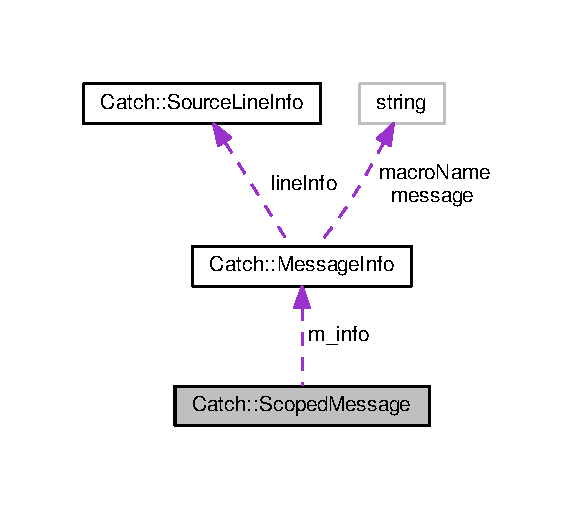
\includegraphics[width=276pt]{classCatch_1_1ScopedMessage__coll__graph}
\end{center}
\end{figure}
\subsection*{Public Member Functions}
\begin{DoxyCompactItemize}
\item 
{\bfseries Scoped\+Message} (\hyperlink{structCatch_1_1MessageBuilder}{Message\+Builder} const \&builder)\hypertarget{classCatch_1_1ScopedMessage_a5cc59f0f2ebe840e6607f83004d49a17}{}\label{classCatch_1_1ScopedMessage_a5cc59f0f2ebe840e6607f83004d49a17}

\end{DoxyCompactItemize}
\subsection*{Public Attributes}
\begin{DoxyCompactItemize}
\item 
\hyperlink{structCatch_1_1MessageInfo}{Message\+Info} {\bfseries m\+\_\+info}\hypertarget{classCatch_1_1ScopedMessage_ae6e1476f389cc6e1586f033b3747b27b}{}\label{classCatch_1_1ScopedMessage_ae6e1476f389cc6e1586f033b3747b27b}

\end{DoxyCompactItemize}


The documentation for this class was generated from the following file\+:\begin{DoxyCompactItemize}
\item 
include/catch.\+hpp\end{DoxyCompactItemize}

\hypertarget{classCatch_1_1Section}{}\section{Catch\+:\+:Section Class Reference}
\label{classCatch_1_1Section}\index{Catch\+::\+Section@{Catch\+::\+Section}}


Inheritance diagram for Catch\+:\+:Section\+:
\nopagebreak
\begin{figure}[H]
\begin{center}
\leavevmode
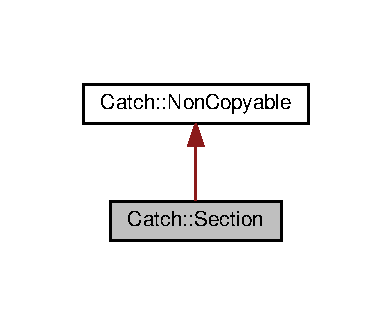
\includegraphics[width=188pt]{classCatch_1_1Section__inherit__graph}
\end{center}
\end{figure}


Collaboration diagram for Catch\+:\+:Section\+:
\nopagebreak
\begin{figure}[H]
\begin{center}
\leavevmode
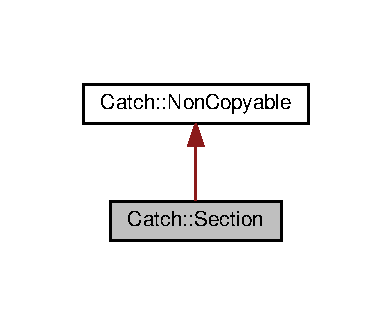
\includegraphics[width=188pt]{classCatch_1_1Section__coll__graph}
\end{center}
\end{figure}
\subsection*{Public Member Functions}
\begin{DoxyCompactItemize}
\item 
{\bfseries Section} (\hyperlink{structCatch_1_1SectionInfo}{Section\+Info} const \&info)\hypertarget{classCatch_1_1Section_a68fd4e51e8981aaa7ddb00d8a6abd099}{}\label{classCatch_1_1Section_a68fd4e51e8981aaa7ddb00d8a6abd099}

\item 
{\bfseries operator bool} () const \hypertarget{classCatch_1_1Section_a6c9be48e8ba0611c4aa601102e706f3b}{}\label{classCatch_1_1Section_a6c9be48e8ba0611c4aa601102e706f3b}

\end{DoxyCompactItemize}


The documentation for this class was generated from the following file\+:\begin{DoxyCompactItemize}
\item 
include/catch.\+hpp\end{DoxyCompactItemize}

\hypertarget{structCatch_1_1SectionEndInfo}{}\section{Catch\+:\+:Section\+End\+Info Struct Reference}
\label{structCatch_1_1SectionEndInfo}\index{Catch\+::\+Section\+End\+Info@{Catch\+::\+Section\+End\+Info}}


Collaboration diagram for Catch\+:\+:Section\+End\+Info\+:\nopagebreak
\begin{figure}[H]
\begin{center}
\leavevmode
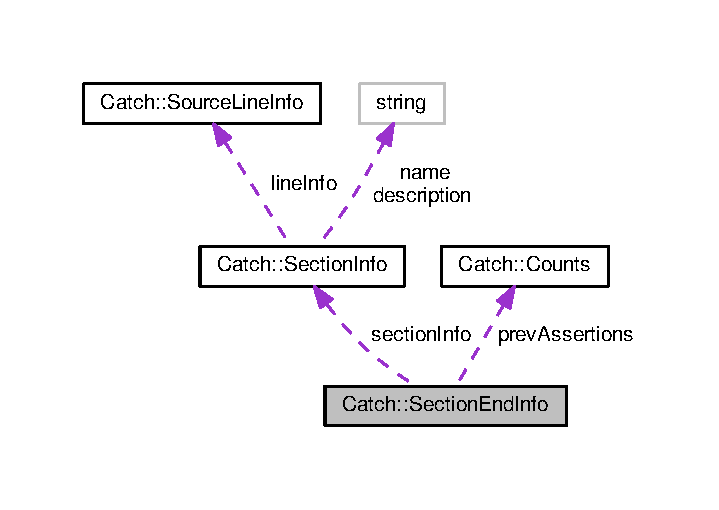
\includegraphics[width=345pt]{structCatch_1_1SectionEndInfo__coll__graph}
\end{center}
\end{figure}
\subsection*{Public Member Functions}
\begin{DoxyCompactItemize}
\item 
{\bfseries Section\+End\+Info} (\hyperlink{structCatch_1_1SectionInfo}{Section\+Info} const \&\+\_\+section\+Info, \hyperlink{structCatch_1_1Counts}{Counts} const \&\+\_\+prev\+Assertions, double \+\_\+duration\+In\+Seconds)\hypertarget{structCatch_1_1SectionEndInfo_abc9381c7c22b6907317ec985ccaa6713}{}\label{structCatch_1_1SectionEndInfo_abc9381c7c22b6907317ec985ccaa6713}

\end{DoxyCompactItemize}
\subsection*{Public Attributes}
\begin{DoxyCompactItemize}
\item 
\hyperlink{structCatch_1_1SectionInfo}{Section\+Info} {\bfseries section\+Info}\hypertarget{structCatch_1_1SectionEndInfo_a2d44793392cb83735d086d726822abe9}{}\label{structCatch_1_1SectionEndInfo_a2d44793392cb83735d086d726822abe9}

\item 
\hyperlink{structCatch_1_1Counts}{Counts} {\bfseries prev\+Assertions}\hypertarget{structCatch_1_1SectionEndInfo_ae70b154cbc05b5dd2901d97f89303d8c}{}\label{structCatch_1_1SectionEndInfo_ae70b154cbc05b5dd2901d97f89303d8c}

\item 
double {\bfseries duration\+In\+Seconds}\hypertarget{structCatch_1_1SectionEndInfo_a7c262f2dab9cff166b8eca620c47eea5}{}\label{structCatch_1_1SectionEndInfo_a7c262f2dab9cff166b8eca620c47eea5}

\end{DoxyCompactItemize}


The documentation for this struct was generated from the following file\+:\begin{DoxyCompactItemize}
\item 
include/catch.\+hpp\end{DoxyCompactItemize}

\hypertarget{structCatch_1_1SectionInfo}{}\section{Catch\+:\+:Section\+Info Struct Reference}
\label{structCatch_1_1SectionInfo}\index{Catch\+::\+Section\+Info@{Catch\+::\+Section\+Info}}


Collaboration diagram for Catch\+:\+:Section\+Info\+:\nopagebreak
\begin{figure}[H]
\begin{center}
\leavevmode
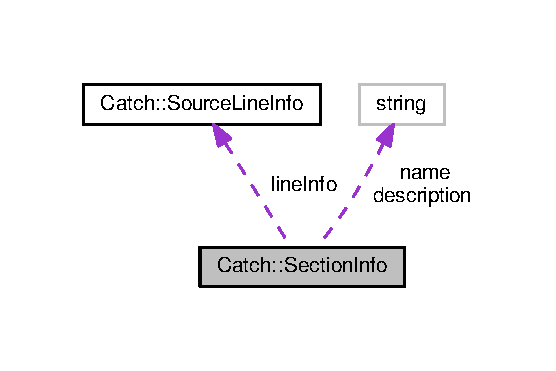
\includegraphics[width=267pt]{structCatch_1_1SectionInfo__coll__graph}
\end{center}
\end{figure}
\subsection*{Public Member Functions}
\begin{DoxyCompactItemize}
\item 
{\bfseries Section\+Info} (\hyperlink{structCatch_1_1SourceLineInfo}{Source\+Line\+Info} const \&\+\_\+line\+Info, std\+::string const \&\+\_\+name, std\+::string const \&\+\_\+description=std\+::string())\hypertarget{structCatch_1_1SectionInfo_a27aff3aaf8b6611f3651b17111a272c6}{}\label{structCatch_1_1SectionInfo_a27aff3aaf8b6611f3651b17111a272c6}

\end{DoxyCompactItemize}
\subsection*{Public Attributes}
\begin{DoxyCompactItemize}
\item 
std\+::string {\bfseries name}\hypertarget{structCatch_1_1SectionInfo_a704c8fc662d309137e0d4f199cb7df58}{}\label{structCatch_1_1SectionInfo_a704c8fc662d309137e0d4f199cb7df58}

\item 
std\+::string {\bfseries description}\hypertarget{structCatch_1_1SectionInfo_a0052060219a6de74bb7ade34d4163a4e}{}\label{structCatch_1_1SectionInfo_a0052060219a6de74bb7ade34d4163a4e}

\item 
\hyperlink{structCatch_1_1SourceLineInfo}{Source\+Line\+Info} {\bfseries line\+Info}\hypertarget{structCatch_1_1SectionInfo_adbc83b8a3507c4acc8ee249e93465711}{}\label{structCatch_1_1SectionInfo_adbc83b8a3507c4acc8ee249e93465711}

\end{DoxyCompactItemize}


The documentation for this struct was generated from the following file\+:\begin{DoxyCompactItemize}
\item 
include/catch.\+hpp\end{DoxyCompactItemize}

\hypertarget{structCatch_1_1SourceLineInfo}{}\section{Catch\+:\+:Source\+Line\+Info Struct Reference}
\label{structCatch_1_1SourceLineInfo}\index{Catch\+::\+Source\+Line\+Info@{Catch\+::\+Source\+Line\+Info}}
\subsection*{Public Member Functions}
\begin{DoxyCompactItemize}
\item 
{\bfseries Source\+Line\+Info} (char const $\ast$\+\_\+file, std\+::size\+\_\+t \+\_\+line) noexcept\hypertarget{structCatch_1_1SourceLineInfo_a48510b82a39a042ab370ed143dd30c10}{}\label{structCatch_1_1SourceLineInfo_a48510b82a39a042ab370ed143dd30c10}

\item 
{\bfseries Source\+Line\+Info} (\hyperlink{structCatch_1_1SourceLineInfo}{Source\+Line\+Info} const \&other)=default\hypertarget{structCatch_1_1SourceLineInfo_a7c44c9986c33a9cf842b791374332d41}{}\label{structCatch_1_1SourceLineInfo_a7c44c9986c33a9cf842b791374332d41}

\item 
{\bfseries Source\+Line\+Info} (\hyperlink{structCatch_1_1SourceLineInfo}{Source\+Line\+Info} \&\&)=default\hypertarget{structCatch_1_1SourceLineInfo_a6614b503b493bbdd3b49a1bd732e0a55}{}\label{structCatch_1_1SourceLineInfo_a6614b503b493bbdd3b49a1bd732e0a55}

\item 
\hyperlink{structCatch_1_1SourceLineInfo}{Source\+Line\+Info} \& {\bfseries operator=} (\hyperlink{structCatch_1_1SourceLineInfo}{Source\+Line\+Info} const \&)=default\hypertarget{structCatch_1_1SourceLineInfo_a1a6cfc0197357ef4e329bb256aa8a354}{}\label{structCatch_1_1SourceLineInfo_a1a6cfc0197357ef4e329bb256aa8a354}

\item 
\hyperlink{structCatch_1_1SourceLineInfo}{Source\+Line\+Info} \& {\bfseries operator=} (\hyperlink{structCatch_1_1SourceLineInfo}{Source\+Line\+Info} \&\&)=default\hypertarget{structCatch_1_1SourceLineInfo_a7fa35372f2bca5e91adc25327b7c753c}{}\label{structCatch_1_1SourceLineInfo_a7fa35372f2bca5e91adc25327b7c753c}

\item 
bool {\bfseries empty} () const noexcept\hypertarget{structCatch_1_1SourceLineInfo_a10a5b5b7dff82971879c2eb8d83f9b3b}{}\label{structCatch_1_1SourceLineInfo_a10a5b5b7dff82971879c2eb8d83f9b3b}

\item 
bool {\bfseries operator==} (\hyperlink{structCatch_1_1SourceLineInfo}{Source\+Line\+Info} const \&other) const noexcept\hypertarget{structCatch_1_1SourceLineInfo_af07e4fdeddf8409b91e4f842f6264cf8}{}\label{structCatch_1_1SourceLineInfo_af07e4fdeddf8409b91e4f842f6264cf8}

\item 
bool {\bfseries operator$<$} (\hyperlink{structCatch_1_1SourceLineInfo}{Source\+Line\+Info} const \&other) const noexcept\hypertarget{structCatch_1_1SourceLineInfo_af77415416919d2d6030b4be085b92f7a}{}\label{structCatch_1_1SourceLineInfo_af77415416919d2d6030b4be085b92f7a}

\end{DoxyCompactItemize}
\subsection*{Public Attributes}
\begin{DoxyCompactItemize}
\item 
char const $\ast$ {\bfseries file}\hypertarget{structCatch_1_1SourceLineInfo_ad65537703e9f08c1fa7777fbc3f0c617}{}\label{structCatch_1_1SourceLineInfo_ad65537703e9f08c1fa7777fbc3f0c617}

\item 
std\+::size\+\_\+t {\bfseries line}\hypertarget{structCatch_1_1SourceLineInfo_a841e5d696c7b9cde24e45e61dd979c77}{}\label{structCatch_1_1SourceLineInfo_a841e5d696c7b9cde24e45e61dd979c77}

\end{DoxyCompactItemize}


The documentation for this struct was generated from the following file\+:\begin{DoxyCompactItemize}
\item 
include/catch.\+hpp\end{DoxyCompactItemize}

\hypertarget{structCatch_1_1Matchers_1_1StdString_1_1StartsWithMatcher}{}\section{Catch\+:\+:Matchers\+:\+:Std\+String\+:\+:Starts\+With\+Matcher Struct Reference}
\label{structCatch_1_1Matchers_1_1StdString_1_1StartsWithMatcher}\index{Catch\+::\+Matchers\+::\+Std\+String\+::\+Starts\+With\+Matcher@{Catch\+::\+Matchers\+::\+Std\+String\+::\+Starts\+With\+Matcher}}


Inheritance diagram for Catch\+:\+:Matchers\+:\+:Std\+String\+:\+:Starts\+With\+Matcher\+:\nopagebreak
\begin{figure}[H]
\begin{center}
\leavevmode
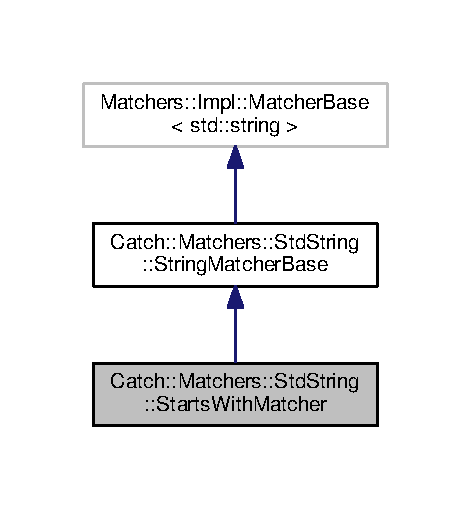
\includegraphics[width=226pt]{structCatch_1_1Matchers_1_1StdString_1_1StartsWithMatcher__inherit__graph}
\end{center}
\end{figure}


Collaboration diagram for Catch\+:\+:Matchers\+:\+:Std\+String\+:\+:Starts\+With\+Matcher\+:\nopagebreak
\begin{figure}[H]
\begin{center}
\leavevmode
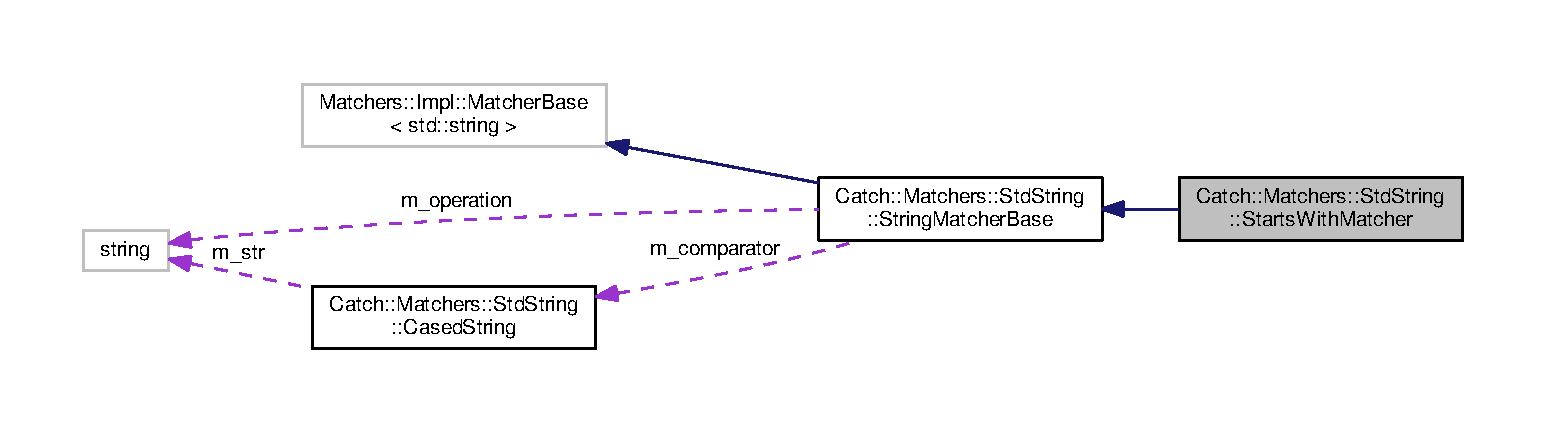
\includegraphics[width=350pt]{structCatch_1_1Matchers_1_1StdString_1_1StartsWithMatcher__coll__graph}
\end{center}
\end{figure}
\subsection*{Public Member Functions}
\begin{DoxyCompactItemize}
\item 
{\bfseries Starts\+With\+Matcher} (\hyperlink{structCatch_1_1Matchers_1_1StdString_1_1CasedString}{Cased\+String} const \&comparator)\hypertarget{structCatch_1_1Matchers_1_1StdString_1_1StartsWithMatcher_a7b86f258bdbd131a6e7bcd94a8977325}{}\label{structCatch_1_1Matchers_1_1StdString_1_1StartsWithMatcher_a7b86f258bdbd131a6e7bcd94a8977325}

\item 
bool {\bfseries match} (std\+::string const \&source) const override\hypertarget{structCatch_1_1Matchers_1_1StdString_1_1StartsWithMatcher_a7da4747aed0c48989d8be59a89e2b7fb}{}\label{structCatch_1_1Matchers_1_1StdString_1_1StartsWithMatcher_a7da4747aed0c48989d8be59a89e2b7fb}

\end{DoxyCompactItemize}
\subsection*{Additional Inherited Members}


The documentation for this struct was generated from the following file\+:\begin{DoxyCompactItemize}
\item 
include/catch.\+hpp\end{DoxyCompactItemize}

\hypertarget{structCatch_1_1StreamEndStop}{}\section{Catch\+:\+:Stream\+End\+Stop Struct Reference}
\label{structCatch_1_1StreamEndStop}\index{Catch\+::\+Stream\+End\+Stop@{Catch\+::\+Stream\+End\+Stop}}
\subsection*{Public Member Functions}
\begin{DoxyCompactItemize}
\item 
std\+::string {\bfseries operator+} () const \hypertarget{structCatch_1_1StreamEndStop_a570db0c412a897ab2748876660428c9e}{}\label{structCatch_1_1StreamEndStop_a570db0c412a897ab2748876660428c9e}

\end{DoxyCompactItemize}


The documentation for this struct was generated from the following file\+:\begin{DoxyCompactItemize}
\item 
include/catch.\+hpp\end{DoxyCompactItemize}

\hypertarget{structCatch_1_1StringMaker}{}\section{Catch\+:\+:String\+Maker$<$ T, typename $>$ Struct Template Reference}
\label{structCatch_1_1StringMaker}\index{Catch\+::\+String\+Maker$<$ T, typename $>$@{Catch\+::\+String\+Maker$<$ T, typename $>$}}
\subsection*{Static Public Member Functions}
\begin{DoxyCompactItemize}
\item 
{\footnotesize template$<$typename Fake  = T$>$ }\\static std\+::enable\+\_\+if$<$\+::\hyperlink{classCatch_1_1Detail_1_1IsStreamInsertable}{Catch\+::\+Detail\+::\+Is\+Stream\+Insertable}$<$ Fake $>$\+::value, std\+::string $>$\+::type {\bfseries convert} (const Fake \&value)\hypertarget{structCatch_1_1StringMaker_ab2c357e22b754802c4b1351257103eb6}{}\label{structCatch_1_1StringMaker_ab2c357e22b754802c4b1351257103eb6}

\item 
{\footnotesize template$<$typename Fake  = T$>$ }\\static std\+::enable\+\_\+if$<$!\+::\hyperlink{classCatch_1_1Detail_1_1IsStreamInsertable}{Catch\+::\+Detail\+::\+Is\+Stream\+Insertable}$<$ Fake $>$\+::value, std\+::string $>$\+::type {\bfseries convert} (const Fake \&value)\hypertarget{structCatch_1_1StringMaker_a68bb548de0e5ad364228b1ca3dd2f561}{}\label{structCatch_1_1StringMaker_a68bb548de0e5ad364228b1ca3dd2f561}

\end{DoxyCompactItemize}


The documentation for this struct was generated from the following file\+:\begin{DoxyCompactItemize}
\item 
include/catch.\+hpp\end{DoxyCompactItemize}

\hypertarget{structCatch_1_1StringMaker_3_01bool_01_4}{}\section{Catch\+:\+:String\+Maker$<$ bool $>$ Struct Template Reference}
\label{structCatch_1_1StringMaker_3_01bool_01_4}\index{Catch\+::\+String\+Maker$<$ bool $>$@{Catch\+::\+String\+Maker$<$ bool $>$}}
\subsection*{Static Public Member Functions}
\begin{DoxyCompactItemize}
\item 
static std\+::string {\bfseries convert} (bool b)\hypertarget{structCatch_1_1StringMaker_3_01bool_01_4_a37e9899c82c4b4515f876f16f8957a77}{}\label{structCatch_1_1StringMaker_3_01bool_01_4_a37e9899c82c4b4515f876f16f8957a77}

\end{DoxyCompactItemize}


The documentation for this struct was generated from the following file\+:\begin{DoxyCompactItemize}
\item 
include/catch.\+hpp\end{DoxyCompactItemize}

\hypertarget{structCatch_1_1StringMaker_3_01Catch_1_1Detail_1_1Approx_01_4}{}\section{Catch\+:\+:String\+Maker$<$ Catch\+:\+:Detail\+:\+:Approx $>$ Struct Template Reference}
\label{structCatch_1_1StringMaker_3_01Catch_1_1Detail_1_1Approx_01_4}\index{Catch\+::\+String\+Maker$<$ Catch\+::\+Detail\+::\+Approx $>$@{Catch\+::\+String\+Maker$<$ Catch\+::\+Detail\+::\+Approx $>$}}
\subsection*{Static Public Member Functions}
\begin{DoxyCompactItemize}
\item 
static std\+::string {\bfseries convert} (\hyperlink{classCatch_1_1Detail_1_1Approx}{Catch\+::\+Detail\+::\+Approx} const \&value)\hypertarget{structCatch_1_1StringMaker_3_01Catch_1_1Detail_1_1Approx_01_4_a8e5015720682fecfbff0f05de19a698f}{}\label{structCatch_1_1StringMaker_3_01Catch_1_1Detail_1_1Approx_01_4_a8e5015720682fecfbff0f05de19a698f}

\end{DoxyCompactItemize}


The documentation for this struct was generated from the following file\+:\begin{DoxyCompactItemize}
\item 
include/catch.\+hpp\end{DoxyCompactItemize}

\hypertarget{structCatch_1_1StringMaker_3_01char_01_5_01_4}{}\section{Catch\+:\+:String\+Maker$<$ char $\ast$ $>$ Struct Template Reference}
\label{structCatch_1_1StringMaker_3_01char_01_5_01_4}\index{Catch\+::\+String\+Maker$<$ char $\ast$ $>$@{Catch\+::\+String\+Maker$<$ char $\ast$ $>$}}
\subsection*{Static Public Member Functions}
\begin{DoxyCompactItemize}
\item 
static std\+::string {\bfseries convert} (char $\ast$str)\hypertarget{structCatch_1_1StringMaker_3_01char_01_5_01_4_a33049e24281ea6fba48bd8817bdd52bd}{}\label{structCatch_1_1StringMaker_3_01char_01_5_01_4_a33049e24281ea6fba48bd8817bdd52bd}

\end{DoxyCompactItemize}


The documentation for this struct was generated from the following file\+:\begin{DoxyCompactItemize}
\item 
include/catch.\+hpp\end{DoxyCompactItemize}

\hypertarget{structCatch_1_1StringMaker_3_01char_01_4}{}\section{Catch\+:\+:String\+Maker$<$ char $>$ Struct Template Reference}
\label{structCatch_1_1StringMaker_3_01char_01_4}\index{Catch\+::\+String\+Maker$<$ char $>$@{Catch\+::\+String\+Maker$<$ char $>$}}
\subsection*{Static Public Member Functions}
\begin{DoxyCompactItemize}
\item 
static std\+::string {\bfseries convert} (char c)\hypertarget{structCatch_1_1StringMaker_3_01char_01_4_a4e3db69a12bb83f3ef89251893e65da5}{}\label{structCatch_1_1StringMaker_3_01char_01_4_a4e3db69a12bb83f3ef89251893e65da5}

\end{DoxyCompactItemize}


The documentation for this struct was generated from the following file\+:\begin{DoxyCompactItemize}
\item 
include/catch.\+hpp\end{DoxyCompactItemize}

\hypertarget{structCatch_1_1StringMaker_3_01char_01const_01_5_01_4}{}\section{Catch\+:\+:String\+Maker$<$ char const $\ast$ $>$ Struct Template Reference}
\label{structCatch_1_1StringMaker_3_01char_01const_01_5_01_4}\index{Catch\+::\+String\+Maker$<$ char const $\ast$ $>$@{Catch\+::\+String\+Maker$<$ char const $\ast$ $>$}}
\subsection*{Static Public Member Functions}
\begin{DoxyCompactItemize}
\item 
static std\+::string {\bfseries convert} (char const $\ast$str)\hypertarget{structCatch_1_1StringMaker_3_01char_01const_01_5_01_4_a20813965ad59cdf6d1f874f47158432d}{}\label{structCatch_1_1StringMaker_3_01char_01const_01_5_01_4_a20813965ad59cdf6d1f874f47158432d}

\end{DoxyCompactItemize}


The documentation for this struct was generated from the following file\+:\begin{DoxyCompactItemize}
\item 
include/catch.\+hpp\end{DoxyCompactItemize}

\hypertarget{structCatch_1_1StringMaker_3_01char[SZ]_4}{}\section{Catch\+:\+:String\+Maker$<$ char\mbox{[}SZ\mbox{]}$>$ Struct Template Reference}
\label{structCatch_1_1StringMaker_3_01char[SZ]_4}\index{Catch\+::\+String\+Maker$<$ char\mbox{[}\+S\+Z\mbox{]}$>$@{Catch\+::\+String\+Maker$<$ char[SZ]$>$}}
\subsection*{Static Public Member Functions}
\begin{DoxyCompactItemize}
\item 
static std\+::string {\bfseries convert} (const char $\ast$str)\hypertarget{structCatch_1_1StringMaker_3_01char[SZ]_4_ab4938ae9fbc5e01cf6a3be615519cefd}{}\label{structCatch_1_1StringMaker_3_01char[SZ]_4_ab4938ae9fbc5e01cf6a3be615519cefd}

\end{DoxyCompactItemize}


The documentation for this struct was generated from the following file\+:\begin{DoxyCompactItemize}
\item 
include/catch.\+hpp\end{DoxyCompactItemize}

\hypertarget{structCatch_1_1StringMaker_3_01double_01_4}{}\section{Catch\+:\+:String\+Maker$<$ double $>$ Struct Template Reference}
\label{structCatch_1_1StringMaker_3_01double_01_4}\index{Catch\+::\+String\+Maker$<$ double $>$@{Catch\+::\+String\+Maker$<$ double $>$}}
\subsection*{Static Public Member Functions}
\begin{DoxyCompactItemize}
\item 
static std\+::string {\bfseries convert} (double value)\hypertarget{structCatch_1_1StringMaker_3_01double_01_4_acaa61529acad2462292c747d34e5f3d2}{}\label{structCatch_1_1StringMaker_3_01double_01_4_acaa61529acad2462292c747d34e5f3d2}

\end{DoxyCompactItemize}


The documentation for this struct was generated from the following file\+:\begin{DoxyCompactItemize}
\item 
include/catch.\+hpp\end{DoxyCompactItemize}

\hypertarget{structCatch_1_1StringMaker_3_01float_01_4}{}\section{Catch\+:\+:String\+Maker$<$ float $>$ Struct Template Reference}
\label{structCatch_1_1StringMaker_3_01float_01_4}\index{Catch\+::\+String\+Maker$<$ float $>$@{Catch\+::\+String\+Maker$<$ float $>$}}
\subsection*{Static Public Member Functions}
\begin{DoxyCompactItemize}
\item 
static std\+::string {\bfseries convert} (float value)\hypertarget{structCatch_1_1StringMaker_3_01float_01_4_a7ffacc6fa46a338200f3fbb2ee078648}{}\label{structCatch_1_1StringMaker_3_01float_01_4_a7ffacc6fa46a338200f3fbb2ee078648}

\end{DoxyCompactItemize}


The documentation for this struct was generated from the following file\+:\begin{DoxyCompactItemize}
\item 
include/catch.\+hpp\end{DoxyCompactItemize}

\hypertarget{structCatch_1_1StringMaker_3_01int_01_4}{}\section{Catch\+:\+:String\+Maker$<$ int $>$ Struct Template Reference}
\label{structCatch_1_1StringMaker_3_01int_01_4}\index{Catch\+::\+String\+Maker$<$ int $>$@{Catch\+::\+String\+Maker$<$ int $>$}}
\subsection*{Static Public Member Functions}
\begin{DoxyCompactItemize}
\item 
static std\+::string {\bfseries convert} (int value)\hypertarget{structCatch_1_1StringMaker_3_01int_01_4_aab096e55fb7283f6ad47b5ca277e22e8}{}\label{structCatch_1_1StringMaker_3_01int_01_4_aab096e55fb7283f6ad47b5ca277e22e8}

\end{DoxyCompactItemize}


The documentation for this struct was generated from the following file\+:\begin{DoxyCompactItemize}
\item 
include/catch.\+hpp\end{DoxyCompactItemize}

\hypertarget{structCatch_1_1StringMaker_3_01long_01_4}{}\section{Catch\+:\+:String\+Maker$<$ long $>$ Struct Template Reference}
\label{structCatch_1_1StringMaker_3_01long_01_4}\index{Catch\+::\+String\+Maker$<$ long $>$@{Catch\+::\+String\+Maker$<$ long $>$}}
\subsection*{Static Public Member Functions}
\begin{DoxyCompactItemize}
\item 
static std\+::string {\bfseries convert} (long value)\hypertarget{structCatch_1_1StringMaker_3_01long_01_4_a1c0c56497813e7a6425c5411d5e66447}{}\label{structCatch_1_1StringMaker_3_01long_01_4_a1c0c56497813e7a6425c5411d5e66447}

\end{DoxyCompactItemize}


The documentation for this struct was generated from the following file\+:\begin{DoxyCompactItemize}
\item 
include/catch.\+hpp\end{DoxyCompactItemize}

\hypertarget{structCatch_1_1StringMaker_3_01long_01long_01_4}{}\section{Catch\+:\+:String\+Maker$<$ long long $>$ Struct Template Reference}
\label{structCatch_1_1StringMaker_3_01long_01long_01_4}\index{Catch\+::\+String\+Maker$<$ long long $>$@{Catch\+::\+String\+Maker$<$ long long $>$}}
\subsection*{Static Public Member Functions}
\begin{DoxyCompactItemize}
\item 
static std\+::string {\bfseries convert} (long long value)\hypertarget{structCatch_1_1StringMaker_3_01long_01long_01_4_a7a58929dca2a14c576d7d6d08bc615d2}{}\label{structCatch_1_1StringMaker_3_01long_01long_01_4_a7a58929dca2a14c576d7d6d08bc615d2}

\end{DoxyCompactItemize}


The documentation for this struct was generated from the following file\+:\begin{DoxyCompactItemize}
\item 
include/catch.\+hpp\end{DoxyCompactItemize}

\hypertarget{structCatch_1_1StringMaker_3_01R_01C_1_1_5_01_4}{}\section{Catch\+:\+:String\+Maker$<$ R C\+:\+:$\ast$ $>$ Struct Template Reference}
\label{structCatch_1_1StringMaker_3_01R_01C_1_1_5_01_4}\index{Catch\+::\+String\+Maker$<$ R C\+::$\ast$ $>$@{Catch\+::\+String\+Maker$<$ R C\+::$\ast$ $>$}}
\subsection*{Static Public Member Functions}
\begin{DoxyCompactItemize}
\item 
static std\+::string {\bfseries convert} (R C\+::$\ast$p)\hypertarget{structCatch_1_1StringMaker_3_01R_01C_1_1_5_01_4_af69c15e0b406e945777137fe4a333731}{}\label{structCatch_1_1StringMaker_3_01R_01C_1_1_5_01_4_af69c15e0b406e945777137fe4a333731}

\end{DoxyCompactItemize}


The documentation for this struct was generated from the following file\+:\begin{DoxyCompactItemize}
\item 
include/catch.\+hpp\end{DoxyCompactItemize}

\hypertarget{structCatch_1_1StringMaker_3_01R_00_01typename_01std_1_1enable__if_3_01is__range_3_01R_01_4_1_1ve8233c20b54b69b4771fbd413409d181}{}\section{Catch\+:\+:String\+Maker$<$ R, typename std\+:\+:enable\+\_\+if$<$ is\+\_\+range$<$ R $>$\+:\+:value \&\&!\+:\+:Catch\+:\+:Detail\+:\+:Is\+Stream\+Insertable$<$ R $>$\+:\+:value $>$\+:\+:type $>$ Struct Template Reference}
\label{structCatch_1_1StringMaker_3_01R_00_01typename_01std_1_1enable__if_3_01is__range_3_01R_01_4_1_1ve8233c20b54b69b4771fbd413409d181}\index{Catch\+::\+String\+Maker$<$ R, typename std\+::enable\+\_\+if$<$ is\+\_\+range$<$ R $>$\+::value \&\&"!\+::\+Catch\+::\+Detail\+::\+Is\+Stream\+Insertable$<$ R $>$\+::value $>$\+::type $>$@{Catch\+::\+String\+Maker$<$ R, typename std\+::enable\+\_\+if$<$ is\+\_\+range$<$ R $>$\+::value \&\&"!\+::\+Catch\+::\+Detail\+::\+Is\+Stream\+Insertable$<$ R $>$\+::value $>$\+::type $>$}}
\subsection*{Static Public Member Functions}
\begin{DoxyCompactItemize}
\item 
static std\+::string {\bfseries convert} (R const \&range)\hypertarget{structCatch_1_1StringMaker_3_01R_00_01typename_01std_1_1enable__if_3_01is__range_3_01R_01_4_1_1ve8233c20b54b69b4771fbd413409d181_ac6088db00103a7482fb9bc04b1603362}{}\label{structCatch_1_1StringMaker_3_01R_00_01typename_01std_1_1enable__if_3_01is__range_3_01R_01_4_1_1ve8233c20b54b69b4771fbd413409d181_ac6088db00103a7482fb9bc04b1603362}

\end{DoxyCompactItemize}


The documentation for this struct was generated from the following file\+:\begin{DoxyCompactItemize}
\item 
include/catch.\+hpp\end{DoxyCompactItemize}

\hypertarget{structCatch_1_1StringMaker_3_01signed_01char_01_4}{}\section{Catch\+:\+:String\+Maker$<$ signed char $>$ Struct Template Reference}
\label{structCatch_1_1StringMaker_3_01signed_01char_01_4}\index{Catch\+::\+String\+Maker$<$ signed char $>$@{Catch\+::\+String\+Maker$<$ signed char $>$}}
\subsection*{Static Public Member Functions}
\begin{DoxyCompactItemize}
\item 
static std\+::string {\bfseries convert} (signed char c)\hypertarget{structCatch_1_1StringMaker_3_01signed_01char_01_4_a5ec41f32916539dc90130539db8222cf}{}\label{structCatch_1_1StringMaker_3_01signed_01char_01_4_a5ec41f32916539dc90130539db8222cf}

\end{DoxyCompactItemize}


The documentation for this struct was generated from the following file\+:\begin{DoxyCompactItemize}
\item 
include/catch.\+hpp\end{DoxyCompactItemize}

\hypertarget{structCatch_1_1StringMaker_3_01signed_01char[SZ]_4}{}\section{Catch\+:\+:String\+Maker$<$ signed char\mbox{[}SZ\mbox{]}$>$ Struct Template Reference}
\label{structCatch_1_1StringMaker_3_01signed_01char[SZ]_4}\index{Catch\+::\+String\+Maker$<$ signed char\mbox{[}\+S\+Z\mbox{]}$>$@{Catch\+::\+String\+Maker$<$ signed char[SZ]$>$}}
\subsection*{Static Public Member Functions}
\begin{DoxyCompactItemize}
\item 
static std\+::string {\bfseries convert} (const char $\ast$str)\hypertarget{structCatch_1_1StringMaker_3_01signed_01char[SZ]_4_ac17d7559af1b1177bae20c1ee028838b}{}\label{structCatch_1_1StringMaker_3_01signed_01char[SZ]_4_ac17d7559af1b1177bae20c1ee028838b}

\end{DoxyCompactItemize}


The documentation for this struct was generated from the following file\+:\begin{DoxyCompactItemize}
\item 
include/catch.\+hpp\end{DoxyCompactItemize}

\hypertarget{structCatch_1_1StringMaker_3_01std_1_1nullptr__t_01_4}{}\section{Catch\+:\+:String\+Maker$<$ std\+:\+:nullptr\+\_\+t $>$ Struct Template Reference}
\label{structCatch_1_1StringMaker_3_01std_1_1nullptr__t_01_4}\index{Catch\+::\+String\+Maker$<$ std\+::nullptr\+\_\+t $>$@{Catch\+::\+String\+Maker$<$ std\+::nullptr\+\_\+t $>$}}
\subsection*{Static Public Member Functions}
\begin{DoxyCompactItemize}
\item 
static std\+::string {\bfseries convert} (std\+::nullptr\+\_\+t)\hypertarget{structCatch_1_1StringMaker_3_01std_1_1nullptr__t_01_4_a131fbb1f5cd68c93aaf30d34e3519e9c}{}\label{structCatch_1_1StringMaker_3_01std_1_1nullptr__t_01_4_a131fbb1f5cd68c93aaf30d34e3519e9c}

\end{DoxyCompactItemize}


The documentation for this struct was generated from the following file\+:\begin{DoxyCompactItemize}
\item 
include/catch.\+hpp\end{DoxyCompactItemize}

\hypertarget{structCatch_1_1StringMaker_3_01std_1_1string_01_4}{}\section{Catch\+:\+:String\+Maker$<$ std\+:\+:string $>$ Struct Template Reference}
\label{structCatch_1_1StringMaker_3_01std_1_1string_01_4}\index{Catch\+::\+String\+Maker$<$ std\+::string $>$@{Catch\+::\+String\+Maker$<$ std\+::string $>$}}
\subsection*{Static Public Member Functions}
\begin{DoxyCompactItemize}
\item 
static std\+::string {\bfseries convert} (const std\+::string \&str)\hypertarget{structCatch_1_1StringMaker_3_01std_1_1string_01_4_ae065b2ecc5c1a6c4409cf06d604bd66d}{}\label{structCatch_1_1StringMaker_3_01std_1_1string_01_4_ae065b2ecc5c1a6c4409cf06d604bd66d}

\end{DoxyCompactItemize}


The documentation for this struct was generated from the following file\+:\begin{DoxyCompactItemize}
\item 
include/catch.\+hpp\end{DoxyCompactItemize}

\hypertarget{structCatch_1_1StringMaker_3_01std_1_1wstring_01_4}{}\section{Catch\+:\+:String\+Maker$<$ std\+:\+:wstring $>$ Struct Template Reference}
\label{structCatch_1_1StringMaker_3_01std_1_1wstring_01_4}\index{Catch\+::\+String\+Maker$<$ std\+::wstring $>$@{Catch\+::\+String\+Maker$<$ std\+::wstring $>$}}
\subsection*{Static Public Member Functions}
\begin{DoxyCompactItemize}
\item 
static std\+::string {\bfseries convert} (const std\+::wstring \&wstr)\hypertarget{structCatch_1_1StringMaker_3_01std_1_1wstring_01_4_a375d49d6281bee4d36d853fa1bd5ebbd}{}\label{structCatch_1_1StringMaker_3_01std_1_1wstring_01_4_a375d49d6281bee4d36d853fa1bd5ebbd}

\end{DoxyCompactItemize}


The documentation for this struct was generated from the following file\+:\begin{DoxyCompactItemize}
\item 
include/catch.\+hpp\end{DoxyCompactItemize}

\hypertarget{structCatch_1_1StringMaker_3_01T_01_5_01_4}{}\section{Catch\+:\+:String\+Maker$<$ T $\ast$ $>$ Struct Template Reference}
\label{structCatch_1_1StringMaker_3_01T_01_5_01_4}\index{Catch\+::\+String\+Maker$<$ T $\ast$ $>$@{Catch\+::\+String\+Maker$<$ T $\ast$ $>$}}
\subsection*{Static Public Member Functions}
\begin{DoxyCompactItemize}
\item 
{\footnotesize template$<$typename U $>$ }\\static std\+::string {\bfseries convert} (U $\ast$p)\hypertarget{structCatch_1_1StringMaker_3_01T_01_5_01_4_a2adbc75c99d71b8323f4052bcb0815c9}{}\label{structCatch_1_1StringMaker_3_01T_01_5_01_4_a2adbc75c99d71b8323f4052bcb0815c9}

\end{DoxyCompactItemize}


The documentation for this struct was generated from the following file\+:\begin{DoxyCompactItemize}
\item 
include/catch.\+hpp\end{DoxyCompactItemize}

\hypertarget{structCatch_1_1StringMaker_3_01T[SZ]_4}{}\section{Catch\+:\+:String\+Maker$<$ T\mbox{[}SZ\mbox{]}$>$ Struct Template Reference}
\label{structCatch_1_1StringMaker_3_01T[SZ]_4}\index{Catch\+::\+String\+Maker$<$ T\mbox{[}\+S\+Z\mbox{]}$>$@{Catch\+::\+String\+Maker$<$ T[SZ]$>$}}
\subsection*{Static Public Member Functions}
\begin{DoxyCompactItemize}
\item 
static std\+::string {\bfseries convert} (T const (\&arr)\mbox{[}SZ\mbox{]})\hypertarget{structCatch_1_1StringMaker_3_01T[SZ]_4_ab10ef3c2111d6faa2ed2f23a1e00c29a}{}\label{structCatch_1_1StringMaker_3_01T[SZ]_4_ab10ef3c2111d6faa2ed2f23a1e00c29a}

\end{DoxyCompactItemize}


The documentation for this struct was generated from the following file\+:\begin{DoxyCompactItemize}
\item 
include/catch.\+hpp\end{DoxyCompactItemize}

\hypertarget{structCatch_1_1StringMaker_3_01unsigned_01char_01_4}{}\section{Catch\+:\+:String\+Maker$<$ unsigned char $>$ Struct Template Reference}
\label{structCatch_1_1StringMaker_3_01unsigned_01char_01_4}\index{Catch\+::\+String\+Maker$<$ unsigned char $>$@{Catch\+::\+String\+Maker$<$ unsigned char $>$}}
\subsection*{Static Public Member Functions}
\begin{DoxyCompactItemize}
\item 
static std\+::string {\bfseries convert} (unsigned char c)\hypertarget{structCatch_1_1StringMaker_3_01unsigned_01char_01_4_a7cddb1df26275b9a8e631466eb122f59}{}\label{structCatch_1_1StringMaker_3_01unsigned_01char_01_4_a7cddb1df26275b9a8e631466eb122f59}

\end{DoxyCompactItemize}


The documentation for this struct was generated from the following file\+:\begin{DoxyCompactItemize}
\item 
include/catch.\+hpp\end{DoxyCompactItemize}

\hypertarget{structCatch_1_1StringMaker_3_01unsigned_01char[SZ]_4}{}\section{Catch\+:\+:String\+Maker$<$ unsigned char\mbox{[}SZ\mbox{]}$>$ Struct Template Reference}
\label{structCatch_1_1StringMaker_3_01unsigned_01char[SZ]_4}\index{Catch\+::\+String\+Maker$<$ unsigned char\mbox{[}\+S\+Z\mbox{]}$>$@{Catch\+::\+String\+Maker$<$ unsigned char[SZ]$>$}}
\subsection*{Static Public Member Functions}
\begin{DoxyCompactItemize}
\item 
static std\+::string {\bfseries convert} (const char $\ast$str)\hypertarget{structCatch_1_1StringMaker_3_01unsigned_01char[SZ]_4_a615e17b55a978cd279442fa293f773f0}{}\label{structCatch_1_1StringMaker_3_01unsigned_01char[SZ]_4_a615e17b55a978cd279442fa293f773f0}

\end{DoxyCompactItemize}


The documentation for this struct was generated from the following file\+:\begin{DoxyCompactItemize}
\item 
include/catch.\+hpp\end{DoxyCompactItemize}

\hypertarget{structCatch_1_1StringMaker_3_01unsigned_01int_01_4}{}\section{Catch\+:\+:String\+Maker$<$ unsigned int $>$ Struct Template Reference}
\label{structCatch_1_1StringMaker_3_01unsigned_01int_01_4}\index{Catch\+::\+String\+Maker$<$ unsigned int $>$@{Catch\+::\+String\+Maker$<$ unsigned int $>$}}
\subsection*{Static Public Member Functions}
\begin{DoxyCompactItemize}
\item 
static std\+::string {\bfseries convert} (unsigned int value)\hypertarget{structCatch_1_1StringMaker_3_01unsigned_01int_01_4_aa0ec816ef8a65664b0524d55d08e2fd9}{}\label{structCatch_1_1StringMaker_3_01unsigned_01int_01_4_aa0ec816ef8a65664b0524d55d08e2fd9}

\end{DoxyCompactItemize}


The documentation for this struct was generated from the following file\+:\begin{DoxyCompactItemize}
\item 
include/catch.\+hpp\end{DoxyCompactItemize}

\hypertarget{structCatch_1_1StringMaker_3_01unsigned_01long_01_4}{}\section{Catch\+:\+:String\+Maker$<$ unsigned long $>$ Struct Template Reference}
\label{structCatch_1_1StringMaker_3_01unsigned_01long_01_4}\index{Catch\+::\+String\+Maker$<$ unsigned long $>$@{Catch\+::\+String\+Maker$<$ unsigned long $>$}}
\subsection*{Static Public Member Functions}
\begin{DoxyCompactItemize}
\item 
static std\+::string {\bfseries convert} (unsigned long value)\hypertarget{structCatch_1_1StringMaker_3_01unsigned_01long_01_4_ae105dc97e4462a86a61b59667f8423c9}{}\label{structCatch_1_1StringMaker_3_01unsigned_01long_01_4_ae105dc97e4462a86a61b59667f8423c9}

\end{DoxyCompactItemize}


The documentation for this struct was generated from the following file\+:\begin{DoxyCompactItemize}
\item 
include/catch.\+hpp\end{DoxyCompactItemize}

\hypertarget{structCatch_1_1StringMaker_3_01unsigned_01long_01long_01_4}{}\section{Catch\+:\+:String\+Maker$<$ unsigned long long $>$ Struct Template Reference}
\label{structCatch_1_1StringMaker_3_01unsigned_01long_01long_01_4}\index{Catch\+::\+String\+Maker$<$ unsigned long long $>$@{Catch\+::\+String\+Maker$<$ unsigned long long $>$}}
\subsection*{Static Public Member Functions}
\begin{DoxyCompactItemize}
\item 
static std\+::string {\bfseries convert} (unsigned long long value)\hypertarget{structCatch_1_1StringMaker_3_01unsigned_01long_01long_01_4_a6a8708af4fc8df3f52d7eab779b6bc6f}{}\label{structCatch_1_1StringMaker_3_01unsigned_01long_01long_01_4_a6a8708af4fc8df3f52d7eab779b6bc6f}

\end{DoxyCompactItemize}


The documentation for this struct was generated from the following file\+:\begin{DoxyCompactItemize}
\item 
include/catch.\+hpp\end{DoxyCompactItemize}

\hypertarget{structCatch_1_1StringMaker_3_01wchar__t_01_5_01_4}{}\section{Catch\+:\+:String\+Maker$<$ wchar\+\_\+t $\ast$ $>$ Struct Template Reference}
\label{structCatch_1_1StringMaker_3_01wchar__t_01_5_01_4}\index{Catch\+::\+String\+Maker$<$ wchar\+\_\+t $\ast$ $>$@{Catch\+::\+String\+Maker$<$ wchar\+\_\+t $\ast$ $>$}}
\subsection*{Static Public Member Functions}
\begin{DoxyCompactItemize}
\item 
static std\+::string {\bfseries convert} (wchar\+\_\+t $\ast$str)\hypertarget{structCatch_1_1StringMaker_3_01wchar__t_01_5_01_4_a6112fe324da2a0b3a690071a228ecd71}{}\label{structCatch_1_1StringMaker_3_01wchar__t_01_5_01_4_a6112fe324da2a0b3a690071a228ecd71}

\end{DoxyCompactItemize}


The documentation for this struct was generated from the following file\+:\begin{DoxyCompactItemize}
\item 
include/catch.\+hpp\end{DoxyCompactItemize}

\hypertarget{structCatch_1_1StringMaker_3_01wchar__t_01const_01_5_01_4}{}\section{Catch\+:\+:String\+Maker$<$ wchar\+\_\+t const $\ast$ $>$ Struct Template Reference}
\label{structCatch_1_1StringMaker_3_01wchar__t_01const_01_5_01_4}\index{Catch\+::\+String\+Maker$<$ wchar\+\_\+t const $\ast$ $>$@{Catch\+::\+String\+Maker$<$ wchar\+\_\+t const $\ast$ $>$}}
\subsection*{Static Public Member Functions}
\begin{DoxyCompactItemize}
\item 
static std\+::string {\bfseries convert} (wchar\+\_\+t const $\ast$str)\hypertarget{structCatch_1_1StringMaker_3_01wchar__t_01const_01_5_01_4_ae7535a1f417ace45ca05e4389334ffeb}{}\label{structCatch_1_1StringMaker_3_01wchar__t_01const_01_5_01_4_ae7535a1f417ace45ca05e4389334ffeb}

\end{DoxyCompactItemize}


The documentation for this struct was generated from the following file\+:\begin{DoxyCompactItemize}
\item 
include/catch.\+hpp\end{DoxyCompactItemize}

\hypertarget{structCatch_1_1Matchers_1_1StdString_1_1StringMatcherBase}{}\section{Catch\+:\+:Matchers\+:\+:Std\+String\+:\+:String\+Matcher\+Base Struct Reference}
\label{structCatch_1_1Matchers_1_1StdString_1_1StringMatcherBase}\index{Catch\+::\+Matchers\+::\+Std\+String\+::\+String\+Matcher\+Base@{Catch\+::\+Matchers\+::\+Std\+String\+::\+String\+Matcher\+Base}}


Inheritance diagram for Catch\+:\+:Matchers\+:\+:Std\+String\+:\+:String\+Matcher\+Base\+:\nopagebreak
\begin{figure}[H]
\begin{center}
\leavevmode
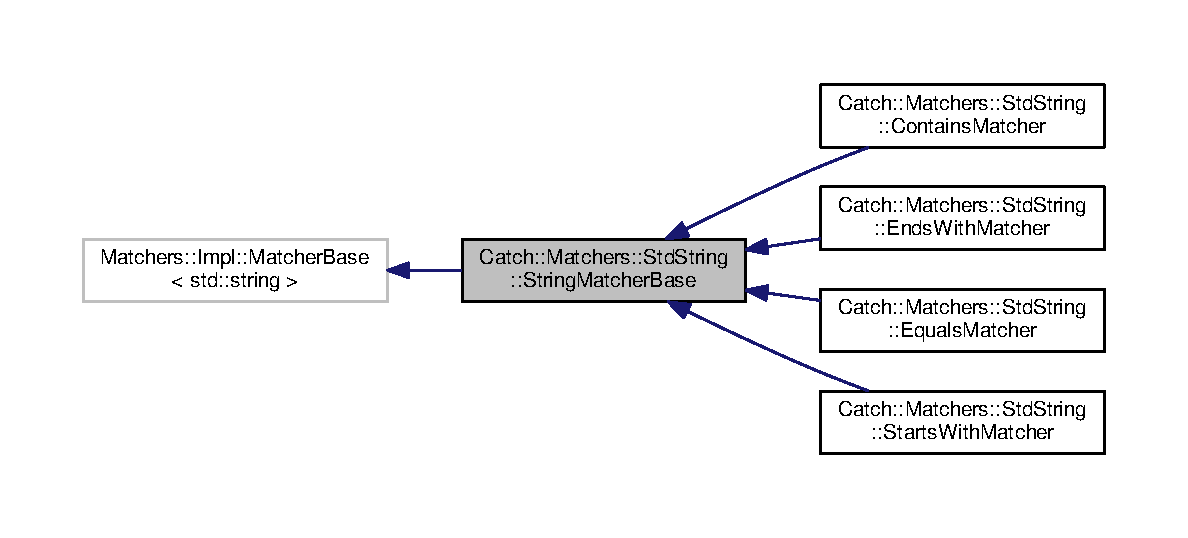
\includegraphics[width=350pt]{structCatch_1_1Matchers_1_1StdString_1_1StringMatcherBase__inherit__graph}
\end{center}
\end{figure}


Collaboration diagram for Catch\+:\+:Matchers\+:\+:Std\+String\+:\+:String\+Matcher\+Base\+:\nopagebreak
\begin{figure}[H]
\begin{center}
\leavevmode
\includegraphics[width=350pt]{structCatch_1_1Matchers_1_1StdString_1_1StringMatcherBase__coll__graph}
\end{center}
\end{figure}
\subsection*{Public Member Functions}
\begin{DoxyCompactItemize}
\item 
{\bfseries String\+Matcher\+Base} (std\+::string const \&operation, \hyperlink{structCatch_1_1Matchers_1_1StdString_1_1CasedString}{Cased\+String} const \&comparator)\hypertarget{structCatch_1_1Matchers_1_1StdString_1_1StringMatcherBase_a3a9b66bae298ae27058478529b4bb39d}{}\label{structCatch_1_1Matchers_1_1StdString_1_1StringMatcherBase_a3a9b66bae298ae27058478529b4bb39d}

\item 
std\+::string {\bfseries describe} () const override\hypertarget{structCatch_1_1Matchers_1_1StdString_1_1StringMatcherBase_a47af030f8cea42a601ffb1000eea5cca}{}\label{structCatch_1_1Matchers_1_1StdString_1_1StringMatcherBase_a47af030f8cea42a601ffb1000eea5cca}

\end{DoxyCompactItemize}
\subsection*{Public Attributes}
\begin{DoxyCompactItemize}
\item 
\hyperlink{structCatch_1_1Matchers_1_1StdString_1_1CasedString}{Cased\+String} {\bfseries m\+\_\+comparator}\hypertarget{structCatch_1_1Matchers_1_1StdString_1_1StringMatcherBase_a17c9f0fe40587070ffe998c193742831}{}\label{structCatch_1_1Matchers_1_1StdString_1_1StringMatcherBase_a17c9f0fe40587070ffe998c193742831}

\item 
std\+::string {\bfseries m\+\_\+operation}\hypertarget{structCatch_1_1Matchers_1_1StdString_1_1StringMatcherBase_a7a25c4b7d863e9a1c406d81efd0f83ca}{}\label{structCatch_1_1Matchers_1_1StdString_1_1StringMatcherBase_a7a25c4b7d863e9a1c406d81efd0f83ca}

\end{DoxyCompactItemize}


The documentation for this struct was generated from the following file\+:\begin{DoxyCompactItemize}
\item 
include/catch.\+hpp\end{DoxyCompactItemize}

\hypertarget{classStringNode}{}\section{String\+Node Class Reference}
\label{classStringNode}\index{String\+Node@{String\+Node}}
\subsection*{Public Member Functions}
\begin{DoxyCompactItemize}
\item 
\hyperlink{classStringNode_a3ac1767041e5519e52ada6e7c5ecbbe4}{String\+Node} ()
\begin{DoxyCompactList}\small\item\em A constructor that creates a node with empty value. \end{DoxyCompactList}\item 
\hyperlink{classStringNode_a1f3433ce567eebdbb4e6eca97c473893}{String\+Node} (string initial\+\_\+text)
\begin{DoxyCompactList}\small\item\em A constructor that creates a node with a string value. \end{DoxyCompactList}\item 
\hyperlink{classStringNode_a2d525c434de4a578a3ff53745865130d}{$\sim$\+String\+Node} ()\hypertarget{classStringNode_a2d525c434de4a578a3ff53745865130d}{}\label{classStringNode_a2d525c434de4a578a3ff53745865130d}

\begin{DoxyCompactList}\small\item\em A destructor that cleans all pointers. \end{DoxyCompactList}\item 
shared\+\_\+ptr$<$ \hyperlink{classStringNode}{String\+Node} $>$ {\bfseries get\+Left\+Node} (void)\hypertarget{classStringNode_a26959d3dfb7ca6cbad4826dfe27f24f6}{}\label{classStringNode_a26959d3dfb7ca6cbad4826dfe27f24f6}

\item 
shared\+\_\+ptr$<$ \hyperlink{classStringNode}{String\+Node} $>$ {\bfseries get\+Right\+Node} (void)\hypertarget{classStringNode_a3803fff2b8a3ca379fbfc1535d882fbd}{}\label{classStringNode_a3803fff2b8a3ca379fbfc1535d882fbd}

\item 
string {\bfseries get\+Text} (void)\hypertarget{classStringNode_a43dce00f3299da71994d88ac0d3c48ee}{}\label{classStringNode_a43dce00f3299da71994d88ac0d3c48ee}

\item 
int \hyperlink{classStringNode_aa87f867d5e9ba8f8263afe8b32cd1df8}{set\+Text} (string new\+Text)
\begin{DoxyCompactList}\small\item\em A method that sets the value of a node. \end{DoxyCompactList}\item 
int \hyperlink{classStringNode_a0496eef4a3ff3c8134ba1ce2e1f01804}{insert\+Node} (string initial\+\_\+new\+\_\+node\+\_\+text)
\begin{DoxyCompactList}\small\item\em A method that create a new node with an initial string chosen. \end{DoxyCompactList}\item 
int \hyperlink{classStringNode_a9deca96372ae91bea728cc9ff5236441}{insert\+Left\+Node} (void)
\begin{DoxyCompactList}\small\item\em A method that creates the a blank left node of an empty branch. \end{DoxyCompactList}\item 
int \hyperlink{classStringNode_a4199a842393aa4d98c3695858b097128}{insert\+Left\+Node} (string initial\+\_\+new\+\_\+node\+\_\+text)
\begin{DoxyCompactList}\small\item\em A method that creates the a setted left node of an empty branch. \end{DoxyCompactList}\item 
int \hyperlink{classStringNode_acdd9f10faab37dd69762ab3774d50775}{insert\+Right\+Node} (void)
\begin{DoxyCompactList}\small\item\em A method that creates the a blank right node of an empty branch. \end{DoxyCompactList}\item 
int \hyperlink{classStringNode_abf313da2479d5c40c2769474948a7398}{insert\+Right\+Node} (string initial\+\_\+new\+\_\+node\+\_\+text)
\begin{DoxyCompactList}\small\item\em A method that creates the a setted right node of an empty branch. \end{DoxyCompactList}\item 
int \hyperlink{classStringNode_acd57ad0e36258a8fada5b092083218f0}{cut\+Node} (void)
\begin{DoxyCompactList}\small\item\em A method that reset each node after cleaning the nodes below it. \end{DoxyCompactList}\item 
int \hyperlink{classStringNode_a8b39a65ddafb6a3324823da77d0af6d0}{clear\+Left} (void)
\begin{DoxyCompactList}\small\item\em A method that resets the left node to null. \end{DoxyCompactList}\item 
int \hyperlink{classStringNode_a778c4554c12fc329fd9d3ecb54c1849b}{clear\+Right} (void)
\begin{DoxyCompactList}\small\item\em A method that resets the right node to null. \end{DoxyCompactList}\end{DoxyCompactItemize}


\subsection{Constructor \& Destructor Documentation}
\index{String\+Node@{String\+Node}!String\+Node@{String\+Node}}
\index{String\+Node@{String\+Node}!String\+Node@{String\+Node}}
\subsubsection[{\texorpdfstring{String\+Node()}{StringNode()}}]{\setlength{\rightskip}{0pt plus 5cm}String\+Node\+::\+String\+Node (
\begin{DoxyParamCaption}
\item[{void}]{}
\end{DoxyParamCaption}
)}\hypertarget{classStringNode_a3ac1767041e5519e52ada6e7c5ecbbe4}{}\label{classStringNode_a3ac1767041e5519e52ada6e7c5ecbbe4}


A constructor that creates a node with empty value. 

Creates a new node with left, right branches and value empties. \index{String\+Node@{String\+Node}!String\+Node@{String\+Node}}
\index{String\+Node@{String\+Node}!String\+Node@{String\+Node}}
\subsubsection[{\texorpdfstring{String\+Node(string initial\+\_\+text)}{StringNode(string initial_text)}}]{\setlength{\rightskip}{0pt plus 5cm}String\+Node\+::\+String\+Node (
\begin{DoxyParamCaption}
\item[{string}]{initial\+\_\+text}
\end{DoxyParamCaption}
)}\hypertarget{classStringNode_a1f3433ce567eebdbb4e6eca97c473893}{}\label{classStringNode_a1f3433ce567eebdbb4e6eca97c473893}


A constructor that creates a node with a string value. 

Creates a new node with left and right branches empty. Sets the value to the string given as param. 
\begin{DoxyParams}{Parameters}
{\em (\+The} & only explicit interface) A valid and already allocated string. \\
\hline
\end{DoxyParams}


\subsection{Member Function Documentation}
\index{String\+Node@{String\+Node}!clear\+Left@{clear\+Left}}
\index{clear\+Left@{clear\+Left}!String\+Node@{String\+Node}}
\subsubsection[{\texorpdfstring{clear\+Left(void)}{clearLeft(void)}}]{\setlength{\rightskip}{0pt plus 5cm}int String\+Node\+::clear\+Left (
\begin{DoxyParamCaption}
\item[{void}]{}
\end{DoxyParamCaption}
)}\hypertarget{classStringNode_a8b39a65ddafb6a3324823da77d0af6d0}{}\label{classStringNode_a8b39a65ddafb6a3324823da77d0af6d0}


A method that resets the left node to null. 

Try to reset the left node If it fails returns an Error(\+Integer 0) else it returns a Success(\+Integer 1). 
\begin{DoxyParams}{Parameters}
{\em (\+The} & only explicit interface)None. \\
\hline
\end{DoxyParams}
\begin{DoxyReturn}{Returns}
An int 0 for Error or 1 for Success 
\end{DoxyReturn}
\index{String\+Node@{String\+Node}!clear\+Right@{clear\+Right}}
\index{clear\+Right@{clear\+Right}!String\+Node@{String\+Node}}
\subsubsection[{\texorpdfstring{clear\+Right(void)}{clearRight(void)}}]{\setlength{\rightskip}{0pt plus 5cm}int String\+Node\+::clear\+Right (
\begin{DoxyParamCaption}
\item[{void}]{}
\end{DoxyParamCaption}
)}\hypertarget{classStringNode_a778c4554c12fc329fd9d3ecb54c1849b}{}\label{classStringNode_a778c4554c12fc329fd9d3ecb54c1849b}


A method that resets the right node to null. 

Try to reset the left node If it fails returns an Error(\+Integer 0) else it returns a Success(\+Integer 1). 
\begin{DoxyParams}{Parameters}
{\em (\+The} & only explicit interface)None. \\
\hline
\end{DoxyParams}
\begin{DoxyReturn}{Returns}
An int 0 for Error or 1 for Success 
\end{DoxyReturn}
\index{String\+Node@{String\+Node}!cut\+Node@{cut\+Node}}
\index{cut\+Node@{cut\+Node}!String\+Node@{String\+Node}}
\subsubsection[{\texorpdfstring{cut\+Node(void)}{cutNode(void)}}]{\setlength{\rightskip}{0pt plus 5cm}int String\+Node\+::cut\+Node (
\begin{DoxyParamCaption}
\item[{void}]{}
\end{DoxyParamCaption}
)}\hypertarget{classStringNode_acd57ad0e36258a8fada5b092083218f0}{}\label{classStringNode_acd57ad0e36258a8fada5b092083218f0}


A method that reset each node after cleaning the nodes below it. 

Try to \+: check if left node is null if it\textquotesingle{}s not, nothing is done. If it\textquotesingle{}s not null, then call a recursion of this method for that node and then resets the left node to null. Then it does the same verification and action to right node. After this, the value of the actual node is cleared. Then return Success(enum 1). If it fails to verify any of them, it returns an Error.(enum 0). Note\+: The actual node it\textquotesingle{}s not deallocated. Just cleared of value. 
\begin{DoxyParams}{Parameters}
{\em (\+The} & only explicit interface)None. \\
\hline
\end{DoxyParams}
\begin{DoxyReturn}{Returns}
An int 0 for Error or 1 for Success 
\end{DoxyReturn}
\index{String\+Node@{String\+Node}!insert\+Left\+Node@{insert\+Left\+Node}}
\index{insert\+Left\+Node@{insert\+Left\+Node}!String\+Node@{String\+Node}}
\subsubsection[{\texorpdfstring{insert\+Left\+Node(void)}{insertLeftNode(void)}}]{\setlength{\rightskip}{0pt plus 5cm}int String\+Node\+::insert\+Left\+Node (
\begin{DoxyParamCaption}
\item[{void}]{}
\end{DoxyParamCaption}
)}\hypertarget{classStringNode_a9deca96372ae91bea728cc9ff5236441}{}\label{classStringNode_a9deca96372ae91bea728cc9ff5236441}


A method that creates the a blank left node of an empty branch. 

Verifies if the left node already exists returns an Error(\+Integer 0). If not creates a new node and sets it\textquotesingle{}s value to empty and returns a Success(Inte-\/ ger 1). 
\begin{DoxyParams}{Parameters}
{\em (\+The} & only explicit interface)None. \\
\hline
\end{DoxyParams}
\begin{DoxyReturn}{Returns}
An int 0 for Error or 1 for Success 
\end{DoxyReturn}
\index{String\+Node@{String\+Node}!insert\+Left\+Node@{insert\+Left\+Node}}
\index{insert\+Left\+Node@{insert\+Left\+Node}!String\+Node@{String\+Node}}
\subsubsection[{\texorpdfstring{insert\+Left\+Node(string initial\+\_\+new\+\_\+node\+\_\+text)}{insertLeftNode(string initial_new_node_text)}}]{\setlength{\rightskip}{0pt plus 5cm}int String\+Node\+::insert\+Left\+Node (
\begin{DoxyParamCaption}
\item[{string}]{initial\+\_\+new\+\_\+node\+\_\+text}
\end{DoxyParamCaption}
)}\hypertarget{classStringNode_a4199a842393aa4d98c3695858b097128}{}\label{classStringNode_a4199a842393aa4d98c3695858b097128}


A method that creates the a setted left node of an empty branch. 

Verifies if the left node already exists returns an Error(\+Integer 0). If not creates a new node and sets it\textquotesingle{}s value to the value of the param then returns a Success(\+Integer 1). 
\begin{DoxyParams}{Parameters}
{\em (\+The} & only explicit interface) A valid and already allocated string which will be the value of the new node. \\
\hline
\end{DoxyParams}
\begin{DoxyReturn}{Returns}
An int 0 for Error or 1 for Success 
\end{DoxyReturn}
\index{String\+Node@{String\+Node}!insert\+Node@{insert\+Node}}
\index{insert\+Node@{insert\+Node}!String\+Node@{String\+Node}}
\subsubsection[{\texorpdfstring{insert\+Node(string initial\+\_\+new\+\_\+node\+\_\+text)}{insertNode(string initial_new_node_text)}}]{\setlength{\rightskip}{0pt plus 5cm}int String\+Node\+::insert\+Node (
\begin{DoxyParamCaption}
\item[{string}]{initial\+\_\+new\+\_\+node\+\_\+text}
\end{DoxyParamCaption}
)}\hypertarget{classStringNode_a0496eef4a3ff3c8134ba1ce2e1f01804}{}\label{classStringNode_a0496eef4a3ff3c8134ba1ce2e1f01804}


A method that create a new node with an initial string chosen. 

verifies if left node is empty, if it is creates a new node and sets it\textquotesingle{}s value to the initial\+\_\+new\+\_\+node\+\_\+text value. Then it\textquotesingle{}ll return a Success which is an enum with value 1. If left node is not empty then it tries the right\+Node. If the right one is empty, creates a new node there and sets it\textquotesingle{}s value to the value of the same argument. Then it\textquotesingle{}ll return a Success which is an enum with value 1. If neither are empty, nothing is done and the method return an Error which is an enum with value 0. 
\begin{DoxyParams}{Parameters}
{\em (\+The} & only explicit interface) A valid and already allocated string which will be the value of the new node. \\
\hline
\end{DoxyParams}
\begin{DoxyReturn}{Returns}
An int 0 for Error or 1 for Success 
\end{DoxyReturn}
\index{String\+Node@{String\+Node}!insert\+Right\+Node@{insert\+Right\+Node}}
\index{insert\+Right\+Node@{insert\+Right\+Node}!String\+Node@{String\+Node}}
\subsubsection[{\texorpdfstring{insert\+Right\+Node(void)}{insertRightNode(void)}}]{\setlength{\rightskip}{0pt plus 5cm}int String\+Node\+::insert\+Right\+Node (
\begin{DoxyParamCaption}
\item[{void}]{}
\end{DoxyParamCaption}
)}\hypertarget{classStringNode_acdd9f10faab37dd69762ab3774d50775}{}\label{classStringNode_acdd9f10faab37dd69762ab3774d50775}


A method that creates the a blank right node of an empty branch. 

Verifies if the right node already exists returns an Error(\+Integer 0). If not creates a new node and sets it\textquotesingle{}s value to empty and returns a Success(Inte-\/ ger 1). 
\begin{DoxyParams}{Parameters}
{\em (\+The} & only explicit interface)None. \\
\hline
\end{DoxyParams}
\begin{DoxyReturn}{Returns}
An int 0 for Error or 1 for Success 
\end{DoxyReturn}
\index{String\+Node@{String\+Node}!insert\+Right\+Node@{insert\+Right\+Node}}
\index{insert\+Right\+Node@{insert\+Right\+Node}!String\+Node@{String\+Node}}
\subsubsection[{\texorpdfstring{insert\+Right\+Node(string initial\+\_\+new\+\_\+node\+\_\+text)}{insertRightNode(string initial_new_node_text)}}]{\setlength{\rightskip}{0pt plus 5cm}int String\+Node\+::insert\+Right\+Node (
\begin{DoxyParamCaption}
\item[{string}]{initial\+\_\+new\+\_\+node\+\_\+text}
\end{DoxyParamCaption}
)}\hypertarget{classStringNode_abf313da2479d5c40c2769474948a7398}{}\label{classStringNode_abf313da2479d5c40c2769474948a7398}


A method that creates the a setted right node of an empty branch. 

Verifies if the right node already exists returns an Error(\+Integer 0). If not creates a new node and sets it\textquotesingle{}s value to the value of the param then returns a Success(\+Integer 1). 
\begin{DoxyParams}{Parameters}
{\em (\+The} & only explicit interface) A valid and already allocated string which will be the value of the new node. \\
\hline
\end{DoxyParams}
\begin{DoxyReturn}{Returns}
An int 0 for Error or 1 for Success 
\end{DoxyReturn}
\index{String\+Node@{String\+Node}!set\+Text@{set\+Text}}
\index{set\+Text@{set\+Text}!String\+Node@{String\+Node}}
\subsubsection[{\texorpdfstring{set\+Text(string new\+Text)}{setText(string newText)}}]{\setlength{\rightskip}{0pt plus 5cm}int String\+Node\+::set\+Text (
\begin{DoxyParamCaption}
\item[{string}]{new\+Text}
\end{DoxyParamCaption}
)}\hypertarget{classStringNode_aa87f867d5e9ba8f8263afe8b32cd1df8}{}\label{classStringNode_aa87f867d5e9ba8f8263afe8b32cd1df8}


A method that sets the value of a node. 

Try to assign a new value to node. If it fails returns an Error(\+Integer 0) else it returns a Success(\+Integer 1). 
\begin{DoxyParams}{Parameters}
{\em (\+The} & only explicit interface)An already existing string. \\
\hline
\end{DoxyParams}
\begin{DoxyReturn}{Returns}
An int 0 for Error or 1 for Success 
\end{DoxyReturn}


The documentation for this class was generated from the following files\+:\begin{DoxyCompactItemize}
\item 
include/stringnode.\+hpp\item 
src/\hyperlink{stringnode_8cpp}{stringnode.\+cpp}\end{DoxyCompactItemize}

\hypertarget{classCatch_1_1StringRef}{}\section{Catch\+:\+:String\+Ref Class Reference}
\label{classCatch_1_1StringRef}\index{Catch\+::\+String\+Ref@{Catch\+::\+String\+Ref}}


{\ttfamily \#include $<$catch.\+hpp$>$}

\subsection*{Public Types}
\begin{DoxyCompactItemize}
\item 
using {\bfseries size\+\_\+type} = std\+::size\+\_\+t\hypertarget{classCatch_1_1StringRef_a06b4db8fc82b197004291cf370b2ba7c}{}\label{classCatch_1_1StringRef_a06b4db8fc82b197004291cf370b2ba7c}

\end{DoxyCompactItemize}
\subsection*{Public Member Functions}
\begin{DoxyCompactItemize}
\item 
{\bfseries String\+Ref} (\hyperlink{classCatch_1_1StringRef}{String\+Ref} const \&other) noexcept\hypertarget{classCatch_1_1StringRef_a2f287267c3a988b288bfd910667c1cfc}{}\label{classCatch_1_1StringRef_a2f287267c3a988b288bfd910667c1cfc}

\item 
{\bfseries String\+Ref} (\hyperlink{classCatch_1_1StringRef}{String\+Ref} \&\&other) noexcept\hypertarget{classCatch_1_1StringRef_a407d5737b94e5a374add5c2794589733}{}\label{classCatch_1_1StringRef_a407d5737b94e5a374add5c2794589733}

\item 
{\bfseries String\+Ref} (char const $\ast$raw\+Chars) noexcept\hypertarget{classCatch_1_1StringRef_aea45f5089c53adac362bff6bd7c40943}{}\label{classCatch_1_1StringRef_aea45f5089c53adac362bff6bd7c40943}

\item 
{\bfseries String\+Ref} (char const $\ast$raw\+Chars, size\+\_\+type size) noexcept\hypertarget{classCatch_1_1StringRef_a320bf235274ebb90dd6af80485af2797}{}\label{classCatch_1_1StringRef_a320bf235274ebb90dd6af80485af2797}

\item 
{\bfseries String\+Ref} (std\+::string const \&std\+String) noexcept\hypertarget{classCatch_1_1StringRef_a7fe41469048f906e9a847798cd335f23}{}\label{classCatch_1_1StringRef_a7fe41469048f906e9a847798cd335f23}

\item 
auto {\bfseries operator=} (\hyperlink{classCatch_1_1StringRef}{String\+Ref} const \&other) noexcept-\/$>$ \hyperlink{classCatch_1_1StringRef}{String\+Ref} \&\hypertarget{classCatch_1_1StringRef_ac330bd7890310e9cab73a82cdfc1b7f4}{}\label{classCatch_1_1StringRef_ac330bd7890310e9cab73a82cdfc1b7f4}

\item 
{\bfseries operator std\+::string} () const \hypertarget{classCatch_1_1StringRef_a7f38055e84bb8d16e23490b2664bb319}{}\label{classCatch_1_1StringRef_a7f38055e84bb8d16e23490b2664bb319}

\item 
void {\bfseries swap} (\hyperlink{classCatch_1_1StringRef}{String\+Ref} \&other) noexcept\hypertarget{classCatch_1_1StringRef_a8a843e39ad3560d10a80524ed926ed63}{}\label{classCatch_1_1StringRef_a8a843e39ad3560d10a80524ed926ed63}

\item 
auto {\bfseries operator==} (\hyperlink{classCatch_1_1StringRef}{String\+Ref} const \&other) const noexcept-\/$>$ bool\hypertarget{classCatch_1_1StringRef_a04c84d944fb51b02552e7ce8de7dbbf0}{}\label{classCatch_1_1StringRef_a04c84d944fb51b02552e7ce8de7dbbf0}

\item 
auto {\bfseries operator!=} (\hyperlink{classCatch_1_1StringRef}{String\+Ref} const \&other) const noexcept-\/$>$ bool\hypertarget{classCatch_1_1StringRef_a015f7b3adee8fe49ebb8172ae2975d21}{}\label{classCatch_1_1StringRef_a015f7b3adee8fe49ebb8172ae2975d21}

\item 
auto {\bfseries operator\mbox{[}$\,$\mbox{]}} (size\+\_\+type index) const noexcept-\/$>$ char\hypertarget{classCatch_1_1StringRef_a803e3617331820a7ad8fea3051d6b094}{}\label{classCatch_1_1StringRef_a803e3617331820a7ad8fea3051d6b094}

\item 
auto {\bfseries empty} () const noexcept-\/$>$ bool\hypertarget{classCatch_1_1StringRef_a326d5d5c97e0e792d66a9056143a922b}{}\label{classCatch_1_1StringRef_a326d5d5c97e0e792d66a9056143a922b}

\item 
auto {\bfseries size} () const noexcept-\/$>$ size\+\_\+type\hypertarget{classCatch_1_1StringRef_aa370158c82397f443a16f96ab3133950}{}\label{classCatch_1_1StringRef_aa370158c82397f443a16f96ab3133950}

\item 
auto {\bfseries number\+Of\+Characters} () const noexcept-\/$>$ size\+\_\+type\hypertarget{classCatch_1_1StringRef_ac1f444eb9a9c7ba18b3f71fc85f3222f}{}\label{classCatch_1_1StringRef_ac1f444eb9a9c7ba18b3f71fc85f3222f}

\item 
auto {\bfseries c\+\_\+str} () const -\/$>$ char const $\ast$\hypertarget{classCatch_1_1StringRef_a1669cb2765e820ca258159676cbd82a5}{}\label{classCatch_1_1StringRef_a1669cb2765e820ca258159676cbd82a5}

\item 
auto {\bfseries substr} (size\+\_\+type start, size\+\_\+type size) const noexcept-\/$>$ \hyperlink{classCatch_1_1StringRef}{String\+Ref}\hypertarget{classCatch_1_1StringRef_a7ce373cbe7068bdc118b8f0fc9a2d44d}{}\label{classCatch_1_1StringRef_a7ce373cbe7068bdc118b8f0fc9a2d44d}

\item 
auto {\bfseries current\+Data} () const noexcept-\/$>$ char const $\ast$\hypertarget{classCatch_1_1StringRef_aa8dd423c873140a92282bc7099ec67fc}{}\label{classCatch_1_1StringRef_aa8dd423c873140a92282bc7099ec67fc}

\end{DoxyCompactItemize}
\subsection*{Friends}
\begin{DoxyCompactItemize}
\item 
struct {\bfseries String\+Ref\+Test\+Access}\hypertarget{classCatch_1_1StringRef_a420e64e1652de1b0d427775781b018f5}{}\label{classCatch_1_1StringRef_a420e64e1652de1b0d427775781b018f5}

\end{DoxyCompactItemize}


\subsection{Detailed Description}
A non-\/owning string class (similar to the forthcoming std\+::string\+\_\+view) Note that, because a \hyperlink{classCatch_1_1StringRef}{String\+Ref} may be a substring of another string, it may not be null terminated. c\+\_\+str() must return a null terminated string, however, and so the \hyperlink{classCatch_1_1StringRef}{String\+Ref} will internally take ownership (taking a copy), if necessary. In theory this ownership is not externally visible -\/ but it does mean (substring) String\+Refs should not be shared between threads. 

The documentation for this class was generated from the following file\+:\begin{DoxyCompactItemize}
\item 
include/catch.\+hpp\end{DoxyCompactItemize}

\hypertarget{classCatch_1_1TestCase}{}\section{Catch\+:\+:Test\+Case Class Reference}
\label{classCatch_1_1TestCase}\index{Catch\+::\+Test\+Case@{Catch\+::\+Test\+Case}}


Inheritance diagram for Catch\+:\+:Test\+Case\+:
\nopagebreak
\begin{figure}[H]
\begin{center}
\leavevmode
\includegraphics[width=188pt]{classCatch_1_1TestCase__inherit__graph}
\end{center}
\end{figure}


Collaboration diagram for Catch\+:\+:Test\+Case\+:
\nopagebreak
\begin{figure}[H]
\begin{center}
\leavevmode
\includegraphics[width=277pt]{classCatch_1_1TestCase__coll__graph}
\end{center}
\end{figure}
\subsection*{Public Member Functions}
\begin{DoxyCompactItemize}
\item 
{\bfseries Test\+Case} (\hyperlink{structCatch_1_1ITestInvoker}{I\+Test\+Invoker} $\ast$test\+Case, \hyperlink{structCatch_1_1TestCaseInfo}{Test\+Case\+Info} \&\&info)\hypertarget{classCatch_1_1TestCase_aae5709fc1cb68e19ab0ac27e1ffd6a76}{}\label{classCatch_1_1TestCase_aae5709fc1cb68e19ab0ac27e1ffd6a76}

\item 
\hyperlink{classCatch_1_1TestCase}{Test\+Case} {\bfseries with\+Name} (std\+::string const \&\+\_\+new\+Name) const \hypertarget{classCatch_1_1TestCase_ab6dbc6c82b7c1680013c67bdedccfc8e}{}\label{classCatch_1_1TestCase_ab6dbc6c82b7c1680013c67bdedccfc8e}

\item 
void {\bfseries invoke} () const \hypertarget{classCatch_1_1TestCase_aac2e028135cc88c3e3aac04650960a6c}{}\label{classCatch_1_1TestCase_aac2e028135cc88c3e3aac04650960a6c}

\item 
\hyperlink{structCatch_1_1TestCaseInfo}{Test\+Case\+Info} const \& {\bfseries get\+Test\+Case\+Info} () const \hypertarget{classCatch_1_1TestCase_a25c03661ab092431cdff10df5c58a5a7}{}\label{classCatch_1_1TestCase_a25c03661ab092431cdff10df5c58a5a7}

\item 
bool {\bfseries operator==} (\hyperlink{classCatch_1_1TestCase}{Test\+Case} const \&other) const \hypertarget{classCatch_1_1TestCase_a40eab521b316c7d476f6b4dd1c33eec8}{}\label{classCatch_1_1TestCase_a40eab521b316c7d476f6b4dd1c33eec8}

\item 
bool {\bfseries operator$<$} (\hyperlink{classCatch_1_1TestCase}{Test\+Case} const \&other) const \hypertarget{classCatch_1_1TestCase_aa5174e85e3aac6e7398dee9c76730324}{}\label{classCatch_1_1TestCase_aa5174e85e3aac6e7398dee9c76730324}

\end{DoxyCompactItemize}
\subsection*{Additional Inherited Members}


The documentation for this class was generated from the following file\+:\begin{DoxyCompactItemize}
\item 
include/catch.\+hpp\end{DoxyCompactItemize}

\hypertarget{structCatch_1_1TestCaseInfo}{}\section{Catch\+:\+:Test\+Case\+Info Struct Reference}
\label{structCatch_1_1TestCaseInfo}\index{Catch\+::\+Test\+Case\+Info@{Catch\+::\+Test\+Case\+Info}}


Inheritance diagram for Catch\+:\+:Test\+Case\+Info\+:
\nopagebreak
\begin{figure}[H]
\begin{center}
\leavevmode
\includegraphics[width=188pt]{structCatch_1_1TestCaseInfo__inherit__graph}
\end{center}
\end{figure}


Collaboration diagram for Catch\+:\+:Test\+Case\+Info\+:
\nopagebreak
\begin{figure}[H]
\begin{center}
\leavevmode
\includegraphics[width=277pt]{structCatch_1_1TestCaseInfo__coll__graph}
\end{center}
\end{figure}
\subsection*{Public Types}
\begin{DoxyCompactItemize}
\item 
enum {\bfseries Special\+Properties} \{ \\*
{\bfseries None} = 0, 
{\bfseries Is\+Hidden} = 1 $<$$<$ 1, 
{\bfseries Should\+Fail} = 1 $<$$<$ 2, 
{\bfseries May\+Fail} = 1 $<$$<$ 3, 
\\*
{\bfseries Throws} = 1 $<$$<$ 4, 
{\bfseries Non\+Portable} = 1 $<$$<$ 5, 
{\bfseries Benchmark} = 1 $<$$<$ 6
 \}\hypertarget{structCatch_1_1TestCaseInfo_a39b232f74b4a7a6f2183b96759027eac}{}\label{structCatch_1_1TestCaseInfo_a39b232f74b4a7a6f2183b96759027eac}

\end{DoxyCompactItemize}
\subsection*{Public Member Functions}
\begin{DoxyCompactItemize}
\item 
{\bfseries Test\+Case\+Info} (std\+::string const \&\+\_\+name, std\+::string const \&\+\_\+class\+Name, std\+::string const \&\+\_\+description, std\+::vector$<$ std\+::string $>$ const \&\+\_\+tags, \hyperlink{structCatch_1_1SourceLineInfo}{Source\+Line\+Info} const \&\+\_\+line\+Info)\hypertarget{structCatch_1_1TestCaseInfo_ad1a6b08b5a83d1c5eb4596b727b5305f}{}\label{structCatch_1_1TestCaseInfo_ad1a6b08b5a83d1c5eb4596b727b5305f}

\item 
bool {\bfseries is\+Hidden} () const \hypertarget{structCatch_1_1TestCaseInfo_a01ac8b11d8c105e5278a239ab5214257}{}\label{structCatch_1_1TestCaseInfo_a01ac8b11d8c105e5278a239ab5214257}

\item 
bool {\bfseries throws} () const \hypertarget{structCatch_1_1TestCaseInfo_a19fb4f0b755956eee8a1fecf713fb7ca}{}\label{structCatch_1_1TestCaseInfo_a19fb4f0b755956eee8a1fecf713fb7ca}

\item 
bool {\bfseries ok\+To\+Fail} () const \hypertarget{structCatch_1_1TestCaseInfo_a64586336bb49bd6e9ef8a089b072a712}{}\label{structCatch_1_1TestCaseInfo_a64586336bb49bd6e9ef8a089b072a712}

\item 
bool {\bfseries expected\+To\+Fail} () const \hypertarget{structCatch_1_1TestCaseInfo_a1ed1c3689c2874c421466945bd3cb75c}{}\label{structCatch_1_1TestCaseInfo_a1ed1c3689c2874c421466945bd3cb75c}

\item 
std\+::string {\bfseries tags\+As\+String} () const \hypertarget{structCatch_1_1TestCaseInfo_aef91e9cfdd8a225d3ad856586e6b52cc}{}\label{structCatch_1_1TestCaseInfo_aef91e9cfdd8a225d3ad856586e6b52cc}

\end{DoxyCompactItemize}
\subsection*{Public Attributes}
\begin{DoxyCompactItemize}
\item 
std\+::string {\bfseries name}\hypertarget{structCatch_1_1TestCaseInfo_a463794e2f5cfead307c93efd134ade36}{}\label{structCatch_1_1TestCaseInfo_a463794e2f5cfead307c93efd134ade36}

\item 
std\+::string {\bfseries class\+Name}\hypertarget{structCatch_1_1TestCaseInfo_a1a5e0825132a38d091defdebbf2f8ce9}{}\label{structCatch_1_1TestCaseInfo_a1a5e0825132a38d091defdebbf2f8ce9}

\item 
std\+::string {\bfseries description}\hypertarget{structCatch_1_1TestCaseInfo_a37fe2db9425bc45f6a33893eac31198e}{}\label{structCatch_1_1TestCaseInfo_a37fe2db9425bc45f6a33893eac31198e}

\item 
std\+::vector$<$ std\+::string $>$ {\bfseries tags}\hypertarget{structCatch_1_1TestCaseInfo_a150a7cbca1dd0c91799ccb14ff822eb0}{}\label{structCatch_1_1TestCaseInfo_a150a7cbca1dd0c91799ccb14ff822eb0}

\item 
std\+::vector$<$ std\+::string $>$ {\bfseries lcase\+Tags}\hypertarget{structCatch_1_1TestCaseInfo_a844e3de9baf6e53cadfba9733c236bfe}{}\label{structCatch_1_1TestCaseInfo_a844e3de9baf6e53cadfba9733c236bfe}

\item 
\hyperlink{structCatch_1_1SourceLineInfo}{Source\+Line\+Info} {\bfseries line\+Info}\hypertarget{structCatch_1_1TestCaseInfo_aa9407b7f442655b51a2aad24b3fa2fd3}{}\label{structCatch_1_1TestCaseInfo_aa9407b7f442655b51a2aad24b3fa2fd3}

\item 
Special\+Properties {\bfseries properties}\hypertarget{structCatch_1_1TestCaseInfo_afc1e84bd7a2e180895a06d9131302af0}{}\label{structCatch_1_1TestCaseInfo_afc1e84bd7a2e180895a06d9131302af0}

\end{DoxyCompactItemize}
\subsection*{Friends}
\begin{DoxyCompactItemize}
\item 
void {\bfseries set\+Tags} (\hyperlink{structCatch_1_1TestCaseInfo}{Test\+Case\+Info} \&test\+Case\+Info, std\+::vector$<$ std\+::string $>$ tags)\hypertarget{structCatch_1_1TestCaseInfo_a0fe44abaf18ae7c26f98a9fc2b08679c}{}\label{structCatch_1_1TestCaseInfo_a0fe44abaf18ae7c26f98a9fc2b08679c}

\end{DoxyCompactItemize}


The documentation for this struct was generated from the following file\+:\begin{DoxyCompactItemize}
\item 
include/catch.\+hpp\end{DoxyCompactItemize}

\hypertarget{structCatch_1_1TestFailureException}{}\section{Catch\+:\+:Test\+Failure\+Exception Struct Reference}
\label{structCatch_1_1TestFailureException}\index{Catch\+::\+Test\+Failure\+Exception@{Catch\+::\+Test\+Failure\+Exception}}


The documentation for this struct was generated from the following file\+:\begin{DoxyCompactItemize}
\item 
include/catch.\+hpp\end{DoxyCompactItemize}

\hypertarget{classCatch_1_1TestInvokerAsMethod}{}\section{Catch\+:\+:Test\+Invoker\+As\+Method$<$ C $>$ Class Template Reference}
\label{classCatch_1_1TestInvokerAsMethod}\index{Catch\+::\+Test\+Invoker\+As\+Method$<$ C $>$@{Catch\+::\+Test\+Invoker\+As\+Method$<$ C $>$}}


Inheritance diagram for Catch\+:\+:Test\+Invoker\+As\+Method$<$ C $>$\+:\nopagebreak
\begin{figure}[H]
\begin{center}
\leavevmode
\includegraphics[width=250pt]{classCatch_1_1TestInvokerAsMethod__inherit__graph}
\end{center}
\end{figure}


Collaboration diagram for Catch\+:\+:Test\+Invoker\+As\+Method$<$ C $>$\+:\nopagebreak
\begin{figure}[H]
\begin{center}
\leavevmode
\includegraphics[width=250pt]{classCatch_1_1TestInvokerAsMethod__coll__graph}
\end{center}
\end{figure}
\subsection*{Public Member Functions}
\begin{DoxyCompactItemize}
\item 
{\bfseries Test\+Invoker\+As\+Method} (void(C\+::$\ast$test\+As\+Method)()) noexcept\hypertarget{classCatch_1_1TestInvokerAsMethod_a119c4bdbbdd95c42859c18541987a1a4}{}\label{classCatch_1_1TestInvokerAsMethod_a119c4bdbbdd95c42859c18541987a1a4}

\item 
void {\bfseries invoke} () const override\hypertarget{classCatch_1_1TestInvokerAsMethod_a8115a06efe273f4112ec0b5452c1b5f2}{}\label{classCatch_1_1TestInvokerAsMethod_a8115a06efe273f4112ec0b5452c1b5f2}

\end{DoxyCompactItemize}


The documentation for this class was generated from the following file\+:\begin{DoxyCompactItemize}
\item 
include/catch.\+hpp\end{DoxyCompactItemize}

\hypertarget{classCatch_1_1Timer}{}\section{Catch\+:\+:Timer Class Reference}
\label{classCatch_1_1Timer}\index{Catch\+::\+Timer@{Catch\+::\+Timer}}
\subsection*{Public Member Functions}
\begin{DoxyCompactItemize}
\item 
void {\bfseries start} ()\hypertarget{classCatch_1_1Timer_a0a56e879e43f36c102bf9ea8b5fc8b72}{}\label{classCatch_1_1Timer_a0a56e879e43f36c102bf9ea8b5fc8b72}

\item 
auto {\bfseries get\+Elapsed\+Nanoseconds} () const -\/$>$ uint64\+\_\+t\hypertarget{classCatch_1_1Timer_a57be5d17ca868a2d6fb1eea84de665cf}{}\label{classCatch_1_1Timer_a57be5d17ca868a2d6fb1eea84de665cf}

\item 
auto {\bfseries get\+Elapsed\+Microseconds} () const -\/$>$ uint64\+\_\+t\hypertarget{classCatch_1_1Timer_a545de17a61a6fee1dbe3de5b0723e5fa}{}\label{classCatch_1_1Timer_a545de17a61a6fee1dbe3de5b0723e5fa}

\item 
auto {\bfseries get\+Elapsed\+Milliseconds} () const -\/$>$ unsigned int\hypertarget{classCatch_1_1Timer_a30aaf458dbb59dd8ac8971c9c62e0eac}{}\label{classCatch_1_1Timer_a30aaf458dbb59dd8ac8971c9c62e0eac}

\item 
auto {\bfseries get\+Elapsed\+Seconds} () const -\/$>$ double\hypertarget{classCatch_1_1Timer_a065e37e3c9eb16bd4dcf41971d8deedc}{}\label{classCatch_1_1Timer_a065e37e3c9eb16bd4dcf41971d8deedc}

\end{DoxyCompactItemize}


The documentation for this class was generated from the following file\+:\begin{DoxyCompactItemize}
\item 
include/catch.\+hpp\end{DoxyCompactItemize}

\hypertarget{structCatch_1_1Totals}{}\section{Catch\+:\+:Totals Struct Reference}
\label{structCatch_1_1Totals}\index{Catch\+::\+Totals@{Catch\+::\+Totals}}


Collaboration diagram for Catch\+:\+:Totals\+:\nopagebreak
\begin{figure}[H]
\begin{center}
\leavevmode
\includegraphics[width=169pt]{structCatch_1_1Totals__coll__graph}
\end{center}
\end{figure}
\subsection*{Public Member Functions}
\begin{DoxyCompactItemize}
\item 
\hyperlink{structCatch_1_1Totals}{Totals} {\bfseries operator-\/} (\hyperlink{structCatch_1_1Totals}{Totals} const \&other) const \hypertarget{structCatch_1_1Totals_abe15cd8a82ba9a4868dd7a542add827c}{}\label{structCatch_1_1Totals_abe15cd8a82ba9a4868dd7a542add827c}

\item 
\hyperlink{structCatch_1_1Totals}{Totals} \& {\bfseries operator+=} (\hyperlink{structCatch_1_1Totals}{Totals} const \&other)\hypertarget{structCatch_1_1Totals_a574015076e54cc405c70b053e3356e43}{}\label{structCatch_1_1Totals_a574015076e54cc405c70b053e3356e43}

\item 
\hyperlink{structCatch_1_1Totals}{Totals} {\bfseries delta} (\hyperlink{structCatch_1_1Totals}{Totals} const \&prev\+Totals) const \hypertarget{structCatch_1_1Totals_a3dee0f599c081a8360c0112fb1dafe8f}{}\label{structCatch_1_1Totals_a3dee0f599c081a8360c0112fb1dafe8f}

\end{DoxyCompactItemize}
\subsection*{Public Attributes}
\begin{DoxyCompactItemize}
\item 
int {\bfseries error} = 0\hypertarget{structCatch_1_1Totals_a6ea14c7de7ea735a14f172a26e08a239}{}\label{structCatch_1_1Totals_a6ea14c7de7ea735a14f172a26e08a239}

\item 
\hyperlink{structCatch_1_1Counts}{Counts} {\bfseries assertions}\hypertarget{structCatch_1_1Totals_a885ded66df752147b30c3d45aa602ec9}{}\label{structCatch_1_1Totals_a885ded66df752147b30c3d45aa602ec9}

\item 
\hyperlink{structCatch_1_1Counts}{Counts} {\bfseries test\+Cases}\hypertarget{structCatch_1_1Totals_adb195fe477aedee2ecea88c888f16506}{}\label{structCatch_1_1Totals_adb195fe477aedee2ecea88c888f16506}

\end{DoxyCompactItemize}


The documentation for this struct was generated from the following file\+:\begin{DoxyCompactItemize}
\item 
include/catch.\+hpp\end{DoxyCompactItemize}

\hypertarget{classCatch_1_1UnaryExpr}{}\section{Catch\+:\+:Unary\+Expr$<$ LhsT $>$ Class Template Reference}
\label{classCatch_1_1UnaryExpr}\index{Catch\+::\+Unary\+Expr$<$ Lhs\+T $>$@{Catch\+::\+Unary\+Expr$<$ Lhs\+T $>$}}


Inheritance diagram for Catch\+:\+:Unary\+Expr$<$ LhsT $>$\+:\nopagebreak
\begin{figure}[H]
\begin{center}
\leavevmode
\includegraphics[width=221pt]{classCatch_1_1UnaryExpr__inherit__graph}
\end{center}
\end{figure}


Collaboration diagram for Catch\+:\+:Unary\+Expr$<$ LhsT $>$\+:\nopagebreak
\begin{figure}[H]
\begin{center}
\leavevmode
\includegraphics[width=221pt]{classCatch_1_1UnaryExpr__coll__graph}
\end{center}
\end{figure}
\subsection*{Public Member Functions}
\begin{DoxyCompactItemize}
\item 
{\bfseries Unary\+Expr} (LhsT lhs)\hypertarget{classCatch_1_1UnaryExpr_ae02f666a1e64da728628aa2033e1d6e7}{}\label{classCatch_1_1UnaryExpr_ae02f666a1e64da728628aa2033e1d6e7}

\end{DoxyCompactItemize}
\subsection*{Additional Inherited Members}


The documentation for this class was generated from the following file\+:\begin{DoxyCompactItemize}
\item 
include/catch.\+hpp\end{DoxyCompactItemize}

\hypertarget{structCatch_1_1Matchers_1_1Vector_1_1UnorderedEqualsMatcher}{}\section{Catch\+:\+:Matchers\+:\+:Vector\+:\+:Unordered\+Equals\+Matcher$<$ T $>$ Struct Template Reference}
\label{structCatch_1_1Matchers_1_1Vector_1_1UnorderedEqualsMatcher}\index{Catch\+::\+Matchers\+::\+Vector\+::\+Unordered\+Equals\+Matcher$<$ T $>$@{Catch\+::\+Matchers\+::\+Vector\+::\+Unordered\+Equals\+Matcher$<$ T $>$}}


Inheritance diagram for Catch\+:\+:Matchers\+:\+:Vector\+:\+:Unordered\+Equals\+Matcher$<$ T $>$\+:\nopagebreak
\begin{figure}[H]
\begin{center}
\leavevmode
\includegraphics[width=237pt]{structCatch_1_1Matchers_1_1Vector_1_1UnorderedEqualsMatcher__inherit__graph}
\end{center}
\end{figure}


Collaboration diagram for Catch\+:\+:Matchers\+:\+:Vector\+:\+:Unordered\+Equals\+Matcher$<$ T $>$\+:\nopagebreak
\begin{figure}[H]
\begin{center}
\leavevmode
\includegraphics[width=237pt]{structCatch_1_1Matchers_1_1Vector_1_1UnorderedEqualsMatcher__coll__graph}
\end{center}
\end{figure}
\subsection*{Public Member Functions}
\begin{DoxyCompactItemize}
\item 
{\bfseries Unordered\+Equals\+Matcher} (std\+::vector$<$ T $>$ const \&target)\hypertarget{structCatch_1_1Matchers_1_1Vector_1_1UnorderedEqualsMatcher_a525905639b2b15b52ddb0bf14bfa19da}{}\label{structCatch_1_1Matchers_1_1Vector_1_1UnorderedEqualsMatcher_a525905639b2b15b52ddb0bf14bfa19da}

\item 
bool {\bfseries match} (std\+::vector$<$ T $>$ const \&vec) const override\hypertarget{structCatch_1_1Matchers_1_1Vector_1_1UnorderedEqualsMatcher_a3ccdd9dd2cd8bdbb8bb121acbb9cb358}{}\label{structCatch_1_1Matchers_1_1Vector_1_1UnorderedEqualsMatcher_a3ccdd9dd2cd8bdbb8bb121acbb9cb358}

\item 
std\+::string {\bfseries describe} () const override\hypertarget{structCatch_1_1Matchers_1_1Vector_1_1UnorderedEqualsMatcher_a7202d811200317abc58c844f663823df}{}\label{structCatch_1_1Matchers_1_1Vector_1_1UnorderedEqualsMatcher_a7202d811200317abc58c844f663823df}

\end{DoxyCompactItemize}


The documentation for this struct was generated from the following file\+:\begin{DoxyCompactItemize}
\item 
include/catch.\+hpp\end{DoxyCompactItemize}

\hypertarget{structCatch_1_1Matchers_1_1Floating_1_1WithinAbsMatcher}{}\section{Catch\+:\+:Matchers\+:\+:Floating\+:\+:Within\+Abs\+Matcher Struct Reference}
\label{structCatch_1_1Matchers_1_1Floating_1_1WithinAbsMatcher}\index{Catch\+::\+Matchers\+::\+Floating\+::\+Within\+Abs\+Matcher@{Catch\+::\+Matchers\+::\+Floating\+::\+Within\+Abs\+Matcher}}


Inheritance diagram for Catch\+:\+:Matchers\+:\+:Floating\+:\+:Within\+Abs\+Matcher\+:
\nopagebreak
\begin{figure}[H]
\begin{center}
\leavevmode
\includegraphics[width=226pt]{structCatch_1_1Matchers_1_1Floating_1_1WithinAbsMatcher__inherit__graph}
\end{center}
\end{figure}


Collaboration diagram for Catch\+:\+:Matchers\+:\+:Floating\+:\+:Within\+Abs\+Matcher\+:
\nopagebreak
\begin{figure}[H]
\begin{center}
\leavevmode
\includegraphics[width=226pt]{structCatch_1_1Matchers_1_1Floating_1_1WithinAbsMatcher__coll__graph}
\end{center}
\end{figure}
\subsection*{Public Member Functions}
\begin{DoxyCompactItemize}
\item 
{\bfseries Within\+Abs\+Matcher} (double target, double margin)\hypertarget{structCatch_1_1Matchers_1_1Floating_1_1WithinAbsMatcher_ac45340b98c41230a7def5bd86c2d870f}{}\label{structCatch_1_1Matchers_1_1Floating_1_1WithinAbsMatcher_ac45340b98c41230a7def5bd86c2d870f}

\item 
bool {\bfseries match} (double const \&matchee) const override\hypertarget{structCatch_1_1Matchers_1_1Floating_1_1WithinAbsMatcher_afa5d8eed57f12c1e5d006471eb0bfe72}{}\label{structCatch_1_1Matchers_1_1Floating_1_1WithinAbsMatcher_afa5d8eed57f12c1e5d006471eb0bfe72}

\item 
std\+::string {\bfseries describe} () const override\hypertarget{structCatch_1_1Matchers_1_1Floating_1_1WithinAbsMatcher_a206a738680f8767af31d3f1835afff3f}{}\label{structCatch_1_1Matchers_1_1Floating_1_1WithinAbsMatcher_a206a738680f8767af31d3f1835afff3f}

\end{DoxyCompactItemize}


The documentation for this struct was generated from the following file\+:\begin{DoxyCompactItemize}
\item 
include/catch.\+hpp\end{DoxyCompactItemize}

\hypertarget{structCatch_1_1Matchers_1_1Floating_1_1WithinUlpsMatcher}{}\section{Catch\+:\+:Matchers\+:\+:Floating\+:\+:Within\+Ulps\+Matcher Struct Reference}
\label{structCatch_1_1Matchers_1_1Floating_1_1WithinUlpsMatcher}\index{Catch\+::\+Matchers\+::\+Floating\+::\+Within\+Ulps\+Matcher@{Catch\+::\+Matchers\+::\+Floating\+::\+Within\+Ulps\+Matcher}}


Inheritance diagram for Catch\+:\+:Matchers\+:\+:Floating\+:\+:Within\+Ulps\+Matcher\+:\nopagebreak
\begin{figure}[H]
\begin{center}
\leavevmode
\includegraphics[width=226pt]{structCatch_1_1Matchers_1_1Floating_1_1WithinUlpsMatcher__inherit__graph}
\end{center}
\end{figure}


Collaboration diagram for Catch\+:\+:Matchers\+:\+:Floating\+:\+:Within\+Ulps\+Matcher\+:\nopagebreak
\begin{figure}[H]
\begin{center}
\leavevmode
\includegraphics[width=226pt]{structCatch_1_1Matchers_1_1Floating_1_1WithinUlpsMatcher__coll__graph}
\end{center}
\end{figure}
\subsection*{Public Member Functions}
\begin{DoxyCompactItemize}
\item 
{\bfseries Within\+Ulps\+Matcher} (double target, int ulps, Floating\+Point\+Kind base\+Type)\hypertarget{structCatch_1_1Matchers_1_1Floating_1_1WithinUlpsMatcher_a836074ae4010275284ab66b2485c6575}{}\label{structCatch_1_1Matchers_1_1Floating_1_1WithinUlpsMatcher_a836074ae4010275284ab66b2485c6575}

\item 
bool {\bfseries match} (double const \&matchee) const override\hypertarget{structCatch_1_1Matchers_1_1Floating_1_1WithinUlpsMatcher_aabda42a0dc5d00f3c5916feb75006b32}{}\label{structCatch_1_1Matchers_1_1Floating_1_1WithinUlpsMatcher_aabda42a0dc5d00f3c5916feb75006b32}

\item 
std\+::string {\bfseries describe} () const override\hypertarget{structCatch_1_1Matchers_1_1Floating_1_1WithinUlpsMatcher_ad9bc8bb7f3abd326580a4bf6cf369b1b}{}\label{structCatch_1_1Matchers_1_1Floating_1_1WithinUlpsMatcher_ad9bc8bb7f3abd326580a4bf6cf369b1b}

\end{DoxyCompactItemize}


The documentation for this struct was generated from the following file\+:\begin{DoxyCompactItemize}
\item 
include/catch.\+hpp\end{DoxyCompactItemize}

%--- End generated contents ---

% Index
\backmatter
\newpage
\phantomsection
\clearemptydoublepage
\addcontentsline{toc}{chapter}{Index}
\printindex

\end{document}
